%% 
%% Copyright 2019-2021 Elsevier Ltd
%% 
%% This file is part of the 'CAS Bundle'.
%% --------------------------------------
%% 
%% It may be distributed under the conditions of the LaTeX Project Public
%% License, either version 1.2 of this license or (at your option) any
%% later version.  The latest version of this license is in
%%    http://www.latex-project.org/lppl.txt
%% and version 1.2 or later is part of all distributions of LaTeX
%% version 1999/12/01 or later.
%% 
%% The list of all files belonging to the 'CAS Bundle' is
%% given in the file `manifest.txt'.
%% 
%% Template article for cas-dc documentclass for 
%% double column output.

\documentclass[a4paper,fleqn]{cas-dc}

% If the frontmatter runs over more than one page
% use the longmktitle option.

%\documentclass[a4paper,fleqn,longmktitle]{cas-dc}

%\usepackage[numbers]{natbib}
%\usepackage[authoryear]{natbib}
\usepackage[authoryear,longnamesfirst]{natbib}

%%%Author macros
\def\tsc#1{\csdef{#1}{\textsc{\lowercase{#1}}\xspace}}
\tsc{WGM}
\tsc{QE}
%%%

% Uncomment and use as if needed
%\newtheorem{theorem}{Theorem}
%\newtheorem{lemma}[theorem]{Lemma}
%\newdefinition{rmk}{Remark}
%\newproof{pf}{Proof}
%\newproof{pot}{Proof of Theorem \ref{thm}}

\usepackage{graphicx}
\usepackage{amsmath}
\usepackage{amssymb}
\usepackage{booktabs,siunitx}
\usepackage{multirow}
\usepackage[utf8]{inputenc}
\usepackage{pgfplots}
\DeclareUnicodeCharacter{2212}{−}
\usepgfplotslibrary{groupplots,dateplot}
\usetikzlibrary{patterns,shapes.arrows}
\pgfplotsset{compat=newest}
\usepackage{caption}
\usepackage{subcaption}
\usepackage{tikz}

\hfuzz=5.002pt % supresses overfull hbox errors

\begin{document}
\let\WriteBookmarks\relax
\def\floatpagepagefraction{1}
\def\textpagefraction{.001}

% Short title
\shorttitle{KGNT-ens: Few-Shot Image Classification with Knowledge Graph Ensembles}    

% Short author
\shortauthors{D. Filipiak, A. Fensel, A. Filipowska}  

% Main title of the paper
\title [mode = title]{KGTN-ens: Few-Shot Image Classification with Knowledge Graph Ensembles}  

% Title footnote mark
% eg: \tnotemark[1]
% \tnotemark[<tnote number>] 

% Title footnote 1.
% eg: \tnotetext[1]{Title footnote text}
% \tnotetext[<tnote number>]{<tnote text>} 

\author[uibk,uw]{Dominik Filipiak}[orcid=0000-0002-4927-9992]
\credit{conceptualization, data curation, formal analysis, investigation, methodology, software, validation, writing -- original draft (85\% of the work in total)}
\cormark[1]
\cortext[mycorrespondingauthor]{Corresponding author}
\ead{dfilipiak@mimuw.edu.pl}
\author[wur,uibk]{Anna Fensel}[orcid=0000-0002-1391-7104]
\credit{conceptualization, funding acquisition, project administration, writing -- review \& editing (10\% of the work in total)}
\ead{anna.fensel@wur.nl}
\author[uep]{Agata Filipowska}[orcid=0000-0002-8425-1872]
\credit{writing -- review \& editing, resources (5\% of the work in total)}
\ead{agata.filipowska@ue.poznan.pl}
\affiliation[uibk]{organization={University of Innsbruck},
            addressline={Innrain 52}, 
            city={Innsbruck},
            postcode={6020}, 
            country={Austria}}
\affiliation[uw]{organization={University of Warsaw},
            addressline={Krakowskie Przedmieście 26/28}, 
            city={Warsaw},
            postcode={00-927}, 
            country={Poland}}
\affiliation[wur]{organization={Wageningen University \& Research},
            addressline={Droevendaalsesteeg 2}, 
            city={Wageningen},
            postcode={6708 PB}, 
            country={The Netherlands}}
\affiliation[uep]{organization={Pozna\'n University of Economics and Business},
            addressline={Al. Niepodległości 10}, 
            city={Poznań},
            postcode={61-875}, 
            country={Poland}}

% For a title note without a number/mark
%\nonumnote{}

% Here goes the abstract
\begin{abstract}
  We propose KGTN-ens, a framework extending the recent Knowledge Graph Transfer Network (KGTN) to be able to incorporate multiple knowledge graph embeddings at a small cost.
  We evaluate it with different combinations of embeddings in a few-shot image classification task.
  We also construct a new knowledge source -- Wikidata embeddings --  and evaluate it with KGTN and KGTN-ens.
  Our approach outperforms KGTN in terms of the top-5 accuracy on the ImageNet-FS dataset for the majority of tested settings.
  The code is available on GitHub: \texttt{The code will be released after the publication}.
\end{abstract}

% Use if graphical abstract is present
%\begin{graphicalabstract}
%\includegraphics{}
%\end{graphicalabstract}

% Research highlights
% \begin{highlights}
% \item We propose KGTN-ens, a framework extending Knowledge Graph Transfer Network to be able to incorporate multiple knowledge graph embeddings at once.
% \item Our experiments indicate that KGTN-ens outperforms the baseline on a few-shot learning task.
% \item We also test the effectiveness of Wikidata embeddings in the Imagenet few-shot learning task.
% \end{highlights}

% Keywords
% Each keyword is seperated by \sep
\begin{keywords}
  Few-shot Image Classification
  \sep 
  Knowledge Graph Enabled AI
  \sep
  Ensemble Learning
\end{keywords}

\maketitle

\section{Introduction}
\label{sec:introduction}
Reliable, fast, and efficient data processing is crucial given the growing volumes of data in both industry and research.
These needs are often addressed by using distributed dataflow frameworks like Spark~\cite{Zaharia2010}, and Flink~\cite{Carbone2015}.
As these frameworks' handle parallelism, distribution, and fault tolerance, they make it easier for users to create scalable data-parallel programs.
The resulting applications can use a variety of compute clusters for data processing.

However, it is still difficult to choose and configure resources in a way that closely meets user-specific goals and constraints~\cite{RajanKCK16,cloudcomputingchallenges2018}.
Numerous strategies have been put forth to assist users, and they can be grouped into two categories:
Model-based techniques~\cite{MaoAMK16,RajanKCK16,ShahAKW19,AlSayehS19,KirchoffXMR19,ChenLLWZ21silhouette,ScheinertTZWAWK21,WillTSBK21,AlSayehMJPS22} often rely on access to historical performance data, however, historical workload execution data is not always available.
Search-based techniques~\cite{AlipourfardLCVY17,HsuNFM18,bilal2020finding,klimovic2018selecta,fekry2020accelerating,MendesCRG20,LiuXL20,SongZLSFDS21} conduct costly profiling runs prior to executing the actual workload utilizing all, or a fraction, of the input data to iteratively create performance models.

Often enough though, the optimized resource configuration is only relevant for the workload at hand. 
Information about the underlying infrastructure are solely obtained implicitly, i.e., by measuring the performance of the target workload in one execution context.
As a consequence, a thorough understanding of utilized resources and their capabilities is lacking and insights gained cannot be easily transferred to other contexts, for instance, when profiling new workloads with different resource demands. 
This requires repeated profiling overhead for reoccurring or comparable workloads that could be avoided, rendering current approaches less resource-efficient than they could be.

Addressing these limitations, we present \emph{Perona}, a novel approach to explicit and robust infrastructure fingerprinting. 
It motivates the usage of common sets and configurations of benchmarking tools to assess the full capabilities of target infrastructures and to make the obtained benchmarking metrics directly comparable.
This explicit fingerprinting operation transparently reveals the characteristics of resources and allows ranking them.
Perona discards irrelevant benchmarking metrics in a data-driven manner by learning a dense, low-dimensional representation of input metric vectors. 
With these, more sophisticated resource decisions can be made for big data analytics, e.g., with regard to scheduling or resource allocations.
To be able to assess a recent benchmark execution, our approach incorporates results of prior benchmark executions, which is particularly useful for detecting resource degradation. 

\emph{Contributions}. The contributions of this paper are:

\begin{itemize}
    \item A novel approach for incorporating infrastructure fingerprinting into model-based methods for optimized resource configuration of workloads through ranking of resources and detection of degrading resource behavior.
    \item A method for context-aware representation learning of benchmark metrics, thereby not only discarding insignificant features but also taking prior benchmark runs and corresponding machine metrics into account. 
    \item An openly available implementation\footnote{\url{https://github.com/dos-group/perona-infrastructure-fingerprinting}} of Perona which we evaluated with regard to common metrics and in interplay with resource configuration methods for distributed dataflows and scientific workflows. 
\end{itemize}

\emph{Outline}. \autoref{sec:related_work} discusses the related work.
\autoref{sec:approach} describes the three main aspects of our approach in detail. 
\autoref{sec:evaluation} presents the results of our evaluation.
\autoref{sec:conclusion} concludes the paper and gives an outlook on future work.
\section{Related work}
\label{sec:related_work}

This section provides a comprehensive overview of the related work.
We start with a brief review of the techniques used for graph neural networks, which are at the core of the KGTN-ens architecture.
Then, we provide a short survey on recent advancements in few-shot learning, which is the main machine learning task solved by the architecture presented in this paper.

\textbf{Graph neural networks.}
In general, Graph neural networks (GNNs) represent a type of neural network, which processes the specified attributes of the graphs.
Task tackled by GNN can be either node-level (such as prediction of a property for each node), edge-level (prediction of a property for each edge), or graph-level (prediction of a property for a whole graph) \citep{sanchez-lengeling2021a}.
Following \cite[]{keriven2019universal}, a crucial feature of GNNs is being either invariant or equivariant to permutations.
That is, for a graph $\mathcal{G}$, network $f$ and a permutation $\Pi$ we have $f(\Pi \star \mathcal{G})=f(\mathcal{G})$ and $f(\Pi \star \mathcal{G})=\Pi \star f(\mathcal{G})$ for invariance and equivariance respectively.
The general-purpose models from the state-of-the-art family of transformer architectures \cite{vaswani2017attention} can be viewed as a special instance of a graph neural network.
Graph neural networks have a wide area of applications, with notable examples in biology (e.g. protein interface prediction) or social networks (e.g. community detection or link prediction).
The less obvious application of GNNs is in the field of image classification, where they are used to learn the prototypes from the knowledge graph embeddings in a few-shot learning setting.

GNNs fall into a broader category of geometric deep learning, which is devoted to the application of deep neural networks on structured non-Euclidean domains, such as graphs, manifolds, meshes, or grids \citep{bronstein2017geometric}.
\cite{gilmer2017neural} proposed \emph{message passing}, which is one of the most important concepts in GNNs.
In this approach, nodes and/or edges can rely on their neighbours in order to create meaningful embeddings iteratively.
\cite{wu2020comprehensive} classify GNNs into four broad categories: recurrent GNNs (RecGNN), convolutional GNNs (ConvGNNs), graph autoencoders (GAEs), and spatial-temporal GNNs (STGNNs).
In this article, Gated Graph Neural Network (GGNN) \citep{li2016gated} are of special interest.
They belong to the category of RecGNNs.
For a fair comparison with KGTN (our baseline), we used GGNN in our experiments.
Following \cite{li2016gated}, the intuitive difference between GNN and GGNN relies on the explicit graph structure of GNNs, which results in more generalisation capabilities at the expense of a less general model of the latter.



\textbf{Few-shot learning.}
While being very effective for numerous vision tasks, one of the main problems with convolutional neural networks (or machine learning in general) is the amount of data they need to provide meaningful predictions.
More recent architectures, such as self-attention models require even more data to train.
On contrary, humans typically require only a few samples to acquire knowledge of seen objects.
One way to tackle this issue is few-shot learning, which is aimed at learning from scarce data.
The complexity of the problem often stems from the required sudden shift of decision boundaries, which is hard to achieve using only a few samples.
A special case of few-shot learning is one-shot learning, which is learning from one labelled sample per class.

Following \cite{song2022comprehensive}, few-shot learning methods can be divided into data augmentation, transfer learning, meta-learning, and multimodal learning.
Data augmentation techniques aim to artificially extend the amount of available data by either transforming input data \citep{chen2019image} or resulting features \citep{chen2019multi}.
Transfer learning focuses on resuing features from networks trained on different datasets with the required amount of data by techniques such as pre-training and fine-tuning or domain adaptation.
Meta-learning includes techniques devoted to learning from data and tasks in order to reuse this knowledge for future downstream tasks.
\cite{finn2017model} proposed a model agnostic meta-learning algorithm MAML.
Specialised approaches to meta-learning include neural architecture search \citep{elsken2019neural} or metric learning \citep{ge2018deep,chicco2021siamese}.
Finally, multimodal learning focuses on the incorporation of external knowledge from heterogenous domains, such as text, speech or knowledge graphs \citep{wang2020large}.

The concept of prototypes was introduced in the work of \cite{snell2017prototypical}, where they proposed prototypical networks focused on learning metric space between class instances and their prototypes.
\cite{hariharan2017low} used representation regularisation and introduced the concept of \emph{hallucinations} in order to enlarge the number of available representations during the training.  
% AWG \cite{gidaris2018dynamic} 
\cite{wang2018low} employed meta-learning techniques and combined them with the aforementioned \emph{hallucinations} to improve few-shot classification metrics.
% LSD \cite{douze2018low} 
A growing number of scholars incorporate structured knowledge into their computer vision research \cite[]{monka2022survey}.
For instance, \cite{li2019large} studied transferable features with the hierarchy which encodes the semantic relations.
Their approach turned out to be applicable to the problem of zero-shot learning as well.
\cite{shen2021model} proposed model agnostic regularisation technique in order to leverage the relationship between graph labels to preserve category neighbourhood.

\section{PROPOSED METHOD}
\label{METHODOLOGY}


\subsection{Input Pipeline}

To illustrate the temporal modeling capacity of our \methodname, we use the most commonly-used Mel-Frequency Cepstral Coefficients (MFCCs) features~\cite{IEMOCAP_CNN1} as the inputs to \methodname. We first set the sampling rate to the raw sampling rate of each corpus and apply framing operation and Hamming window to each speech signal with 50-ms frame length and 12.5-ms shift. Then, the speech signal undergoes a mel-scale triangular filter bank analysis after performing a 2,048-point fast Fourier transform to each frame. Finally, each frame of the MFCCs is processed by the discrete cosine transformation, where the first 39 coefficients are extracted to obtain the low-frequency envelope and high-frequency details.

\begin{table*}[]
\renewcommand{\arraystretch}{1.0}
\centering
\small
\caption{The overall results of different SOTA methods on 6 SER corpora. Evaluation measures are UAR(\%) / WAR(\%). The `-' implies the lack of this measure. Furthermore, the superscripts indicate different evaluation settings. The `$^{*}$' implies a 10-fold cross-validation with 90\% and 10\% samples in train and test sets respectively, whose model is only evaluated at the last epoch. The `$^{**}$' implies a 10-fold cross-validation that 90\% of samples are used for training and 10\% for both validating and testing. Note that methods without superscript means that there is no source code to verify their specific experimental details.}

\begin{tabular*}{1\linewidth}{@{\extracolsep{\fill}}lcc|lcc|lcc}
\toprule[1.5pt]
\textbf{Model}    & \textbf{Year}     & \textbf{CASIA}         & \textbf{Model}   & \textbf{Year}      & \textbf{EMODB}         & \textbf{Model}   & \textbf{Year}      & \textbf{EMOVO}         \\
\midrule
DT-SVM~\cite{DT_SVM}  & 2019     & 85.08 / 85.08          & TSP+INCA~\cite{TSP_INCA} & 2021       & 89.47 / 90.09           & RM+CNN~\cite{RM_CNN} & 2021       & 68.93 / 68.93            \\
TLFMRF~\cite{TLFMRF} & 2020        & 85.83 / 85.83           & GM-TCN$^{**}$~\cite{GM_TCNet} & 2022       & 90.48 / 91.39            & SVM~\cite{MFMC_SVM} & 2021        & 73.30 / 73.30          \\
GM-TCN$^{**}$~\cite{GM_TCNet} & 2022       & 90.17 / 90.17          &  LightSER$^{**}$~\cite{IEMOCAP_CNN2}   & 2022    & 94.15 / 94.21        & TSP+INCA~\cite{TSP_INCA} & 2021       & 79.08 / 79.08           \\
CPAC$^{**}$~\cite{CPAC_IJCAI}  & 2022        & 92.75 / 92.75           & CPAC$^{**}$~\cite{CPAC_IJCAI}  & 2022         & 94.22 / 94.95          & CPAC$^{**}$~\cite{CPAC_IJCAI}  & 2022       & 85.40 / 85.40           \\\midrule
\textbf{\methodname}$^{*}$ & 2023 & \textbf{91.08 / 91.08}&
\textbf{\methodname}$^{*}$ & 2023 & \textbf{89.19 / 90.28}&
\textbf{\methodname}$^{*}$ & 2023 & \textbf{86.56 / 86.56}\\
\textbf{\methodname}$^{**}$ & 2023 & 94.67 / 94.67& 
\textbf{\methodname}$^{**}$ & 2023 & 95.17 / 95.70&
\textbf{\methodname}$^{**}$ & 2023 & 92.00 / 92.00

\\\midrule\midrule
\textbf{Model}   & \textbf{Year}      & \textbf{IEMOCAP}         & \textbf{Model}    & \textbf{Year}     & \textbf{RAVDESS}       & \textbf{Model}    & \textbf{Year}     & \textbf{SAVEE}     \\
\midrule
MHA+DRN~\cite{IEMOCAP_DRN}  & 2019     & 67.40 / ~~~~-~~~~            & CNN+INCA~\cite{INCA_CNN} & 2021        & ~~~~-~~~~ / 85.00          & DCNN~\cite{DCNN} & 2020       & ~~~~-~~~~ / 82.10           \\
CNN+Bi-GRU~\cite{IEMOCAP_GRU}  & 2020     & 71.72 / 70.39          & TSP+INCA~\cite{TSP_INCA} & 2021        & 87.43 / 87.43           &    TSP+INCA~\cite{TSP_INCA} & 2021        & 83.38 / 84.79         \\
SPU+MSCNN~\cite{IEMOCAP_CNN1} & 2021   & 68.40 / 66.60             & GM-TCN$^{**}$~\cite{GM_TCNet} & 2022       & 87.64 / 87.35           &     CPAC$^{**}$~\cite{CPAC_IJCAI}  & 2022         & 83.69 / 85.63           \\
LightSER$^{**}$~\cite{IEMOCAP_CNN2}   & 2022    & 70.76 / 70.23           & CPAC$^{**}$~\cite{CPAC_IJCAI}  & 2022         & 88.41 / 89.03          & GM-TCN$^{**}$~\cite{GM_TCNet} & 2022       & 83.88 / 86.02        \\\midrule
\textbf{\methodname}$^{*}$ & 2023 & \textbf{69.00 / 68.29}&
\textbf{\methodname}$^{*}$ & 2023 & \textbf{90.04 / 90.07}&
\textbf{\methodname}$^{*}$ & 2023 & \textbf{77.26 / 79.36}\\
\textbf{\methodname}$^{**}$ & 2023 & 72.50 / 71.65&
\textbf{\methodname}$^{**}$ & 2023 & 91.93 / 92.08&
\textbf{\methodname}$^{**}$ & 2023 & 86.07 / 87.71\\\bottomrule[1.5pt]

\end{tabular*}
\label{tab:SOTA}
\end{table*}


\subsection {Temporal-aware Bi-direction Multi-scale Network}

We propose a novel temporal emotional modeling approach called \methodname, which learns long-range emotional dependencies from the forward and backward directions and captures multi-scale features at frame-level. Fig.~\ref{fig:architecture} presents the detailed network architecture of \methodname. For learning multi-scale representations with long-range dependencies, the \methodname consists of $n$ Temporal-Aware Blocks (TABs) in both forward and backward directions with different temporal receptive fields. Next, we detail each component.

\noindent\textbf{Temporal-aware block.}\quad We design the TAB to capture dependencies between different frames and automatically select the affective frames, severing as a core unit of \methodname. As shown in Fig.~\ref{fig:architecture}, $\mathcal{T}$ denotes a TAB, each of which consists of two sub-blocks and a sigmoid function $\sigma(\cdot)$ to learn temporal attention maps $\mathcal{A}$, so as to produce the temporal-aware feature $\mat{F}$ by element-wise production of the input and $\mathcal{A}$. For the two identical sub-blocks of the $j$-th TAB $\mathcal{T}_j$, each sub-block starts by adding a DC Conv with the exponentially increasing dilated rate $2^{j-1}$ and causal constraint. 
The dilated convolution enlarges and refines the receptive field and the causal constraint ensures that the future information is not leaked to the past. 
The DC Conv is then followed by a batch normalization, a ReLU function, and a spatial dropout.

\noindent\textbf{Bi-direction temporal modeling.}\quad To integrate complementary information from the past and the future for the judgement of emotion polarity and modeling long-range temporal dependencies, we devise a novel bi-direction architecture based on the multi-scale features as shown in Fig.~\ref{fig:architecture}.
Formally, for the $\vec{\mathcal{T}}_{j+1}$ in the forward direction with the input $\vec{\mat{F}}_{j}$ from previous TAB, the output $\vec{\mat{F}}_{j+1}$ is given by Eq.~\eqref{eq:forward}:
\begin{align}
    \vec{\mat{F}}_{j+1}= \mathcal{A}(\vec{\mat{F}}_{j})\odot \vec{\mat{F}}_{j},\label{eq:forward}\\
    \cev{\mat{F}}_{j+1}= \mathcal{A}(\cev{\mat{F}}_{j})\odot \cev{\mat{F}}_{j},\label{eq:back}
\end{align}
where $\vec{\mat{F}}_{0}$ comes from the output of the first $1\times 1$ Conv layer and the backward direction can be defined similarly in Eq.~\eqref{eq:back}.

We then combine bidirectional semantic dependencies and compact global contextual representation at utterance level to perceive context as follows:
\begin{align}
    \vct{g}_j&=\mathcal{G}(\vec{\mat{F}}_{j}+\cev{\mat{F}}_{j}) \label{equ:GAP_feat},
\end{align}
where the global temporal pooling operation $\mathcal{G}$ takes an average over temporal dimension, yielding a representation vector for one specific receptive field from the $j$-th TAB.%~\cite{global_temporal_pooling}


\noindent\textbf{Multi-scale dynamic fusion.}\quad Furthermore, since the pronunciation habits (\eg speed or pause time) vary from speaker to speaker, the utterances have the characteristics of temporal scale variation. SER benefits from taking dynamic temporal receptive fields into consideration. We design the dynamic fusion module to adaptively process speech input at different scales, aiming to determine suitable temporal scale for the current input during the training phase. We adopt a weighted summation operation to fuse the features with Dynamic Receptive Fields (DRF) fusion weights $\mat{w}_\text{drf}$ from different TABs. The DRF fusion is defined as follows: 
\begin{align}
    \vct{g}_\text{drf}=\sum\nolimits_{j=1}^{n}w_j\vct{g}_j,  \label{equ:dynamic_rf}
\end{align}
where $\mat{w}_\text{drf} = [w_1,w_2,\ldots,w_{n}]\T$ are trainable parameters. 

Once the emotional representation $\mat{w}_\text{drf}$ is generated with great discriminability, we can simply use one fully-connected layer with the softmax function for emotion classification.

\section{Evaluation}
\label{sec:results}

This section contains the results of the conducted experiments.
First, we introduce the used knowledge sources -- semantic similarity graph, WordNet and Wikidata.
Then, we describe the evaluation of KGTN-ens with different combinations of embeddings and compare them with the previous work.
Finally, we provide a detailed analysis and ablation studies.

\subsection{Knowledge sources}
\label{sec:results_knowledge}

In our evaluation, we use three different sources of knowledge, which can be the backbone of KGTMs: \emph{hierarchy}, \emph{glove}, and \emph{wiki}.
The first two have been proposed by \cite{chen2020knowledge}.
The wiki graph is constructed on top of Wikidata, a collaborative knowledge graph connected to Wikipedia \citep{vrandevcic2014wikidata}.
In this subsection, we discuss the preparation of these knowledge sources in detail.

\textbf{Semantic similarity graph (\emph{glove}).}
The first source of knowledge is built from GLoVe word embeddings \citep{pennington2014glove}.
For two words $w_i$ and $w_j$, their semantic distance $d_{i,j}$ is defined as the Euclidean distance between their GLoVe embeddings $\mathbf{f}_i^w$ and $\mathbf{f}_j^w$.
Following \cite{chen2020knowledge}, the final correlation coefficient $a_{i,j}$ is obtained using the following function:
\begin{equation}
    \lambda^{d_{i,j} - \min d_{i,k}, \forall k \neq i},
    \label{eq:monotonic_function}
\end{equation}
where $\lambda=0.4$ and $a_{ii}=1$.

\textbf{WordNet category distance (\emph{hierarchy}).}
This source of knowledge is built from the WordNet hierarchy -- a popular lexical database of English \citep{miller1995wordnet}.
Since ImageNet classes are based on WordNet, the WordNet hierarchy can be used to measure the distance between two classes.
This time the distance $d_{i,j}$ is defined as the number of common ancestors of the two words (categories) $w_i$ and $w_j$.
The output is processed similarly to Equation \eqref{eq:monotonic_function}, except that the $\lambda$ parameter is set to 0.5.

\textbf{Wikidata embeddings (\emph{wiki}).}
The last source of knowledge is built from the Wikidata embeddings.
The mapping between the ImageNet classes and Wikidata is provided by \cite{filipiak2021mapping}.
Having the mapping, the class-corresponding entities from Wikidata can be embedded and used as a class prototypes.
Although there exist some datasets of Wikidata embeddings, they are often incomplete.
Most importantly, they does not contain all the embeddings of ImageNet classes.
Wembedder \citep{nielsen2017wembedder} offers 100-dimensional Wikidata embeddings made using the word2vec algorithm \citep{mikolov2013efficient}, but it bases on an incomplete dump of Wikidata and does not contain all the classes nedded in the ImageNet-FS dataset.
\cite{zhu2019graphvite} proposed Graphvite, a general graph embedding engine.
\textit{Wikidata5m} is a large dataset of 5 million Wikidata entities, which is used to train the embeddings.
The framework comes with embeddings created using numerous popular algorithms, such as TransE, DistMult, ComplEx, SimplE, RotatE, and QuatE.
However, 891 out of 1000 entities used in the ImageNet are embedded, which was not enough for performing the experiment.

We used the pre-trained 200-dimensional embeddings of Wikidata entities from PyTorch BigGraph \citep{lerer2019pytorch}, which are publicly available\footnote{\url{https://torchbiggraph.readthedocs.io/en/latest/pretrained_embeddings.html}}.
The embeddings were prepared using the full Wikidata dump from 2019-03-06.
All but three entities were directly mapped to embeddings to their Wikidata ID.
Three entities (\texttt{Q1295201}, \texttt{Q98957255}, \texttt{Q89579852}) could not be instantly matched -- they were manually matched to \texttt{"grocery store"@en}, \texttt{"cricket"@en}, and \texttt{Q655301} respectively.
Having the mapping, now we create an embedding array, ordered as the mappings in the original KGTN paper (that is, as a $1000 \times 200$ array, where 200 denotes the dimensionality of a single embedding).
The same function from Equation~\eqref{eq:monotonic_function} was used to generate final correlations between the embeddings, although this time $\lambda=0.32$ was used (see Section \ref{sec:details_ablation}).

\subsection{Experiment results}
\label{sec:results_experiment}

In this subsection, we present the results of the conducted experiments.
We describe the evaluation data -- the experiment has been conducted on ImageNet-FS dataset.
The training hyperparameters and the setup is also described.
We also describe the evaluation protocol, as well as the evaluation metrics.
Finally, we present the results of the experiments and compare them with the previous work.

\textbf{Data.}
Similarly to Chen et al., our approach has been evaluated on ImageNet-FS, a popular benchmark for few-shot learning task.
ImageNet-FS contains 1,000 classes from ImageNet Large Scale Visual Recognition Challenge 2012 \citep{ILSVRC15}, of which 389 belongs to the base category and 611 to the novel category.
193 base classes and 300 novel classes are used for training and cross-validation, whereas the test phase is performed on the remaining 196 categories and 311 novel classes.
Base categories consist of around 1280 train and 50 test images per each class.
The authors of KGTN also evaluated their solution against a larger dataset, ImageNet-6K, which contains 6,000 classes (of which 1,00 belongs to the novel category).
Unfortunately, we were unable to test KGTN-ens using this dataset, since it has not been made public nor available to us at the time of writing this paper.

\textbf{Training.}
To enable fair comparison, we used the same 2-step training and evaluation procedures as in KGTN.
Stochastic gradient descent (SGD) was used to train the model with a batch size equal to 256 (divided equally for base and novel classes), a momentum of 0.9, and a weight decay of 0.0005.
The learning rate is initially set at 0.1 and divided by 30 at every 30 epochs.
In general, we used the same hyperparameters as in KGTN unless stated otherwise.

\textbf{Setup.}
All the experiments have been conducted on a single NVIDIA GeForce RTX 2080 Ti GPU.
We used the code released by the authors of KGTN and modified it to support the KGTN-ens approach.
PyTorch \cite{paszke2017automatic} was used to conduct the experiments.
The code will be released after the publication of this article.

\textbf{Evaluation.}
Following previous work in few-shot learning, we report our evaluation results in terms of the top-5 accuracy of novel and all (base + novel) classes in the $k$-shot learning task, where $k \in \{1,2,5, 10\}$ is the number of classes in the novel category.
Following \cite{hariharan2017low} and \cite{chen2020knowledge}, we repeat each experiment five times and report the averaged values of the top-5 accuracy.
Table~\ref{tab:results} shows the classification results compared with some of the recent state-of-the-art benchmarks.
Figure \ref{fig:kgtn-ens_performance} presents the top-5 accuracy of the KGTN-ens model on ImageNet-FS.
Of three possible combinations of the three sources of knowledge, the KGTN-ens model performed best with the combination of \emph{hierarchy} and \emph{glove}.
Notably, it performed better than KGTN with these two sources of knowledge alone.
Compared to KGTN (with inner product similarity and glove embeddings), the KGTN-ens model (inner product, max ens. function, glove and hierarchy embeddings) achieved +0.63, +0.58, +0.43, +0.26 pp. top-5 accuracy on novel classes for $k \in \{ 1, 2, 5, 10\}$ respectively.
The smaller the $k$, the higher the performance gain.
It also beats the more recent graph-based framework proposed by \cite{shen2021model} by +1.73/+1.18/+0.20 pp. top-5 accuracy on novel classes.
For the all classes, the KGTN-ens model achieved +0.26, +0.25, +0.32, --0.04 pp. top-5 accuracy compared to the same KGTN model for $k \in \{ 1, 2, 5, 10\}$ respectively.

\begin{table*}
    \centering
    \caption{Top-5 accuracy on \emph{novel} and \emph{all} subsets on ImageNet-FS. All the methods used ResNet-50 as a feature extractor. Partially based on the data provided by \cite{chen2020knowledge}.}
    \label{tab:results}
    \begin{tabular}{l rrrr rrrr}
    \toprule
     & \multicolumn{4}{c}{novel} & \multicolumn{4}{c}{all} \\ \cmidrule(lr){2-5} \cmidrule(lr){6-9}
     & \multicolumn{1}{c}{1} & \multicolumn{1}{c}{2} & \multicolumn{1}{c}{5} & \multicolumn{1}{c}{10} & \multicolumn{1}{c}{1} & \multicolumn{1}{c}{2} & \multicolumn{1}{c}{5} & \multicolumn{1}{c}{10} \\
    \midrule
    MN \cite{vinyals2016matching} & 53.5 & 63.5 & 72.7 & 77.4 & 64.9 & 71.0 & 77.0 & 80.2 \\
    PN \cite{snell2017prototypical} & 49.6 & 64.0 & 74.4 & 78.1 & 61.4 & 71.4 & 78.0 & 80.0 \\
    SGM \cite{hariharan2017low} & 54.3 & 67.0 & 77.4 & 81.9 & 60.7 & 71.6 & 80.2 &  83.6 \\
    SGM w/ G \cite{hariharan2017low} & 52.9 & 64.9 & 77.3 & 82.0 & 63.9 & 71.9 & 80.2 & 83.6 \\
    AWG \cite{gidaris2018dynamic} & 53.9 & 65.5 & 75.9 & 80.3 & 65.1 & 72.3 & 79.1 & 82.1 \\
    PMN \cite{wang2018low} & 53.3 & 65.2 & 75.9 & 80.1 & 64.8 & 72.1 & 78.8 & 81.7 \\
    PMN w/ G \cite{wang2018low} & 54.7 & 66.8 & 77.4 & 81.4 & 65.7 & 73.5 & 80.2 & 82.8 \\
    LSD \cite{douze2018low} & 57.7 & 66.9 & 73.8 & 77.6 & -- & -- & -- & -- \\
    KTCH \cite{li2019large} & 58.1 & 67.3 & 77.6 & 81.8 & -- & -- & -- & -- \\
    IDeMe-Net \cite{chen2019image} & 60.1 & 69.6 & 77.4 & 80.2 & -- & -- & -- & -- \\
    KGTN-CosSim \cite{chen2020knowledge} & 61.4 & 70.4 & 78.4 & 82.2 &  67.7 & 74.7 & 80.9 & \textbf{83.6} \\
    KGTN-PearsonCorr \cite{chen2020knowledge} & 61.5 & 70.6 & 78.5 & 82.3 & 67.5 & 74.4 & 80.7 & 83.5 \\
    KGTN-InnerProduct \cite{chen2020knowledge} & 62.1 & 70.9 & 78.4 & 82.3 & 68.3 & 75.2 & 80.8 & 83.5 \\
    SGM with graph regularisation \cite{shen2021model} & 61.1 & 70.3 & 78.6 & -- & -- & -- & -- & -- \\
    KGTN-ens (ours) & \textbf{62.73} & \textbf{71.48} & \textbf{78.83} & \textbf{82.56} & \textbf{68.58} & \textbf{75.45} & \textbf{81.12} & 83.46 \\
    \bottomrule
    \end{tabular}    
\end{table*}

\begin{figure}
    \centering    
    \begin{subfigure}[b]{.5\textwidth}
        \centering
        % This file was created with tikzplotlib v0.10.1.
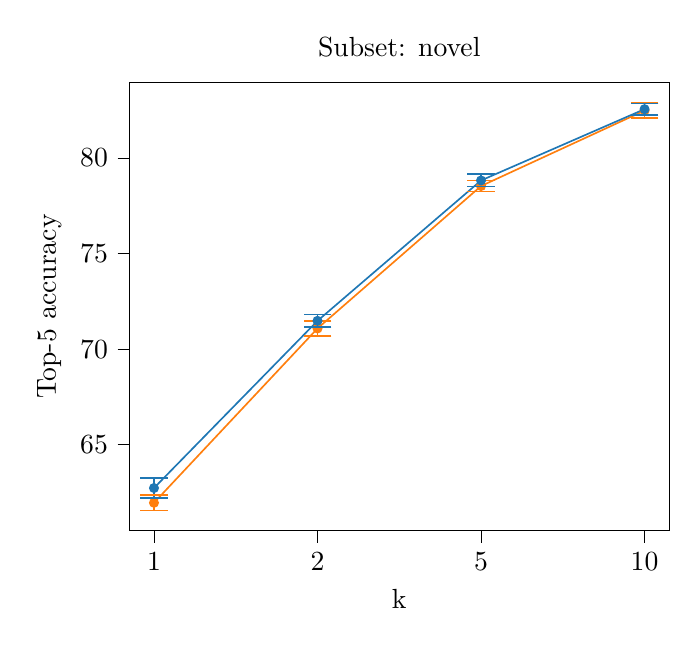
\begin{tikzpicture}

\definecolor{darkgray176}{RGB}{176,176,176}
\definecolor{darkorange25512714}{RGB}{255,127,14}
\definecolor{lightgray204}{RGB}{204,204,204}
\definecolor{steelblue31119180}{RGB}{31,119,180}

\begin{axis}[
legend cell align={left},
legend style={
  fill opacity=0.8,
  draw opacity=1,
  text opacity=1,
  at={(0.97,0.03)},
  anchor=south east,
  draw=lightgray204
},
tick align=outside,
tick pos=left,
title={Subset: novel},
x grid style={darkgray176},
xlabel={k},
xmin=-0.15, xmax=3.15,
xtick style={color=black},
xtick={0,1,2,3},
xtick={0,1,2,3},
xtick={0,1,2,3},
xtick={0,1,2,3},
xtick={0,1,2,3},
xtick={0,1,2,3},
xticklabels={1,2,5,10},
xticklabels={1,2,5,10},
xticklabels={1,2,5,10},
xticklabels={1,2,5,10},
xticklabels={1,2,5,10},
xticklabels={1,2,5,10},
y grid style={darkgray176},
ylabel={Top-5 accuracy},
ymin=60.4949736662386, ymax=83.9517212149162,
ytick style={color=black}
]

\path [draw=darkorange25512714, semithick]
(axis cs:0,61.5611894639058)
--(axis cs:0,62.3616401180878);

\path [draw=darkorange25512714, semithick]
(axis cs:1,70.6993290183528)
--(axis cs:1,71.4665873803611);

\path [draw=darkorange25512714, semithick]
(axis cs:2,78.2504533010468)
--(axis cs:2,78.8170708147088);

\path [draw=darkorange25512714, semithick]
(axis cs:3,82.0791248078314)
--(axis cs:3,82.885505417249);

\path [draw=steelblue31119180, semithick]
(axis cs:0,62.1986523071615)
--(axis cs:0,63.2675856349607);

\path [draw=steelblue31119180, semithick]
(axis cs:1,71.1533675453303)
--(axis cs:1,71.8099765061167);

\path [draw=steelblue31119180, semithick]
(axis cs:2,78.502138954217)
--(axis cs:2,79.1493079911206);

\path [draw=steelblue31119180, semithick]
(axis cs:3,82.2532127531485)
--(axis cs:3,82.8606136134109);


\addplot [semithick, darkorange25512714, mark=-, mark size=5, mark options={solid}, only marks]
table {%
0 61.5611894639058
1 70.6993290183528
2 78.2504533010468
3 82.0791248078314
};
% \addlegendentry{KGTN (baseline)}
\addplot [semithick, darkorange25512714, mark=-, mark size=5, mark options={solid}, only marks]
table {%
0 62.3616401180878
1 71.4665873803611
2 78.8170708147088
3 82.885505417249
};
% \addlegendentry{KGTN (baseline)}
\addplot [semithick, darkorange25512714, mark=*, mark size=1.5, mark options={solid}]
table {%
0 61.9614147909968
1 71.0829581993569
2 78.5337620578778
3 82.4823151125402
};
% \addlegendentry{KGTN (baseline)}
\addplot [semithick, steelblue31119180, mark=-, mark size=5, mark options={solid}, only marks]
table {%
0 62.1986523071615
1 71.1533675453303
2 78.502138954217
3 82.2532127531485
};
% \addlegendentry{KGTN (baseline)}
\addplot [semithick, steelblue31119180, mark=-, mark size=5, mark options={solid}, only marks]
table {%
0 63.2675856349607
1 71.8099765061167
2 79.1493079911206
3 82.8606136134109
};
% \addlegendentry{KGTN (baseline)}
\addplot [semithick, steelblue31119180, mark=*, mark size=1.5, mark options={solid}]
table {%
0 62.7331189710611
1 71.4816720257235
2 78.8257234726688
3 82.5569131832797
};
% \addlegendentry{KGTN-ens (ours)}
\end{axis}

\end{tikzpicture}

        % \caption{Subset: novell}
        \label{fig:max_novel}
    \end{subfigure}  
    % \hfill
    % \begin{subfigure}[b]{.5\textwidth}
    %     \centering
    %     % This file was created with tikzplotlib v0.10.1.
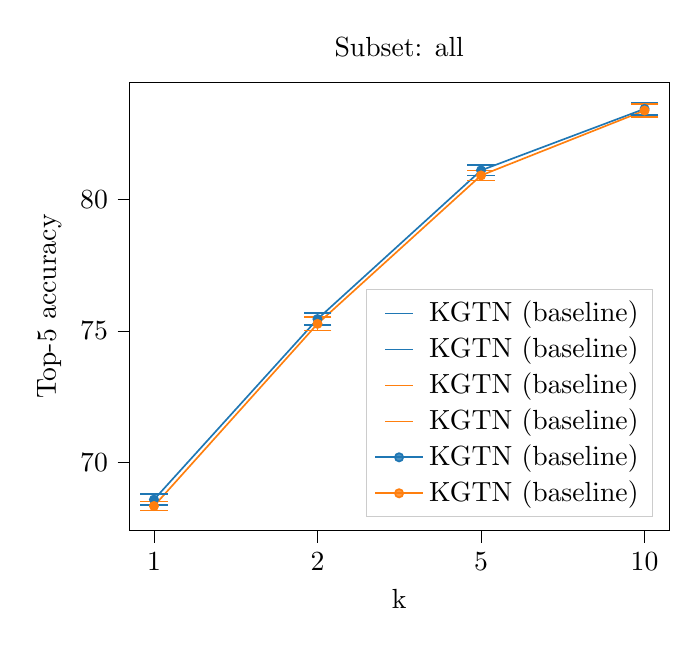
\begin{tikzpicture}

\definecolor{darkgray176}{RGB}{176,176,176}
\definecolor{darkorange25512714}{RGB}{255,127,14}
\definecolor{lightgray204}{RGB}{204,204,204}
\definecolor{steelblue31119180}{RGB}{31,119,180}

\begin{axis}[
legend cell align={left},
legend style={
  fill opacity=0.8,
  draw opacity=1,
  text opacity=1,
  at={(0.97,0.03)},
  anchor=south east,
  draw=lightgray204
},
tick align=outside,
tick pos=left,
title={Subset: all},
x grid style={darkgray176},
xlabel={k},
xmin=-0.15, xmax=3.15,
xtick style={color=black},
xtick={0,1,2,3},
xtick={0,1,2,3},
xtick={0,1,2,3},
xtick={0,1,2,3},
xtick={0,1,2,3},
xtick={0,1,2,3},
xticklabels={1,2,5,10},
xticklabels={1,2,5,10},
xticklabels={1,2,5,10},
xticklabels={1,2,5,10},
xticklabels={1,2,5,10},
xticklabels={1,2,5,10},
y grid style={darkgray176},
ylabel={Top-5 accuracy},
ymin=67.3915172035368, ymax=84.4639924361267,
ytick style={color=black}
]
\path [draw=steelblue31119180, semithick]
(axis cs:0,68.3752395381539)
--(axis cs:0,68.7845237754556);

\path [draw=steelblue31119180, semithick]
(axis cs:1,75.2277093123702)
--(axis cs:1,75.6819553819099);

\path [draw=steelblue31119180, semithick]
(axis cs:2,80.9190331624066)
--(axis cs:2,81.3152863642206);

\path [draw=steelblue31119180, semithick]
(axis cs:3,83.2327392245262)
--(axis cs:3,83.6879708346454);

\path [draw=darkorange25512714, semithick]
(axis cs:0,68.1675388050182)
--(axis cs:0,68.5046505440943);

\path [draw=darkorange25512714, semithick]
(axis cs:1,75.0244654083379)
--(axis cs:1,75.5222801537923);

\path [draw=darkorange25512714, semithick]
(axis cs:2,80.735300768388)
--(axis cs:2,81.1124309870361);

\path [draw=darkorange25512714, semithick]
(axis cs:3,83.1508832173259)
--(axis cs:3,83.6420161909581);

\addplot [semithick, steelblue31119180, mark=-, mark size=5, mark options={solid}, only marks]
table {%
0 68.3752395381539
1 75.2277093123702
2 80.9190331624066
3 83.2327392245262
};
\addlegendentry{KGTN (baseline)}
\addplot [semithick, steelblue31119180, mark=-, mark size=5, mark options={solid}, only marks]
table {%
0 68.7845237754556
1 75.6819553819099
2 81.3152863642206
3 83.6879708346454
};
\addlegendentry{KGTN (baseline)}
\addplot [semithick, darkorange25512714, mark=-, mark size=5, mark options={solid}, only marks]
table {%
0 68.1675388050182
1 75.0244654083379
2 80.735300768388
3 83.1508832173259
};
\addlegendentry{KGTN (baseline)}
\addplot [semithick, darkorange25512714, mark=-, mark size=5, mark options={solid}, only marks]
table {%
0 68.5046505440943
1 75.5222801537923
2 81.1124309870361
3 83.6420161909581
};
\addlegendentry{KGTN (baseline)}
\addplot [semithick, steelblue31119180, mark=*, mark size=1.5, mark options={solid}]
table {%
0 68.5798816568047
1 75.45483234714
2 81.1171597633136
3 83.4603550295858
};
\addlegendentry{KGTN (baseline)}
\addplot [semithick, darkorange25512714, mark=*, mark size=1.5, mark options={solid}]
table {%
0 68.3360946745562
1 75.2733727810651
2 80.923865877712
3 83.396449704142
};
\addlegendentry{KGTN (baseline)}
\end{axis}

\end{tikzpicture}

    %     % \caption{Subset: all}
    %     \label{fig:max_all}
    % \end{subfigure}
    \caption{KNGT-ens (blue) performance mean top-5 accuracy with compared to the KGTN (orange) over 5 runs. KGNT-ens uses glove and hierarchy graphs combined with the max ensembling function. Horizontal lines indicate standard deviations. }
    \label{fig:kgtn-ens_performance}
\end{figure}

\subsection{Details and ablation studies}
\label{sec:details_ablation}

This subsection provides more details on the KGTN-ens model and its ablation studies.
We analyse the impact of the following factors on the performance of the KGTN-ens model: adjacency matrices, used embeddings, ensembling method, similarity function, and variance of the results.

\textbf{Adjacency matrix analysis.}
Since glove knowledge graph was the most effective for KGTN, we assume that wiki should roughly resemble it in terms of its distribution.
In order to investigate the similarity between distributions, adjacency matrices have been created using pairwise euclidean distances.
While glove and wiki are normal-like, the distribution for hierarchy is bimodal and most of the distances are the highest ones (Figure \ref{fig:ablation_dist}).
To assess the correlation between adjacency matrices, Mantel tests have been performed (Table \ref{tab:mantel_raw}).
The values marked as processed were run through Equation \eqref{eq:monotonic_function}.
Correlations of the processed matrices are visibly higher compared to raw ones, especially regarding glove and wiki).
The highest correlation has been observed between glove and wiki.

\begin{table}
    \centering
    \caption{Descriptive statistics about the adjacency matrices.}
    \label{tab:ablation_adjacency_stats}
    \begin{tabular}{ll rrrr}
    \toprule
    & KG & Min & Avg & Max & Std \\
    \midrule
    \multirow{3}{*}{Raw} & hierarchy & 0.00 & 9.76 & 10.00 & 1.20 \\
    & glove & 0.00 & 8.52 & 14.31 & 1.29 \\
    & wiki & 0.00 & 5.82 & 12.73 & 1.32 \\ \cmidrule(){2-6}
    \multirow{3}{*}{Processed} & hierachy   & 0.00 & 0.01 & 2.00 & 0.07 \\
    & glove      & 0.00 & 0.05 & 2.00 & 0.11 \\
    & wiki       & 0.00 & 0.08 & 2.00 & 0.14 \\ \bottomrule
\end{tabular}
\end{table}

\begin{figure}%
    % \centering
    \begin{subfigure}{.5\textwidth}
        \centering
        \label{fig:ablation_dist_raw}
        % This file was created with tikzplotlib v0.10.1.
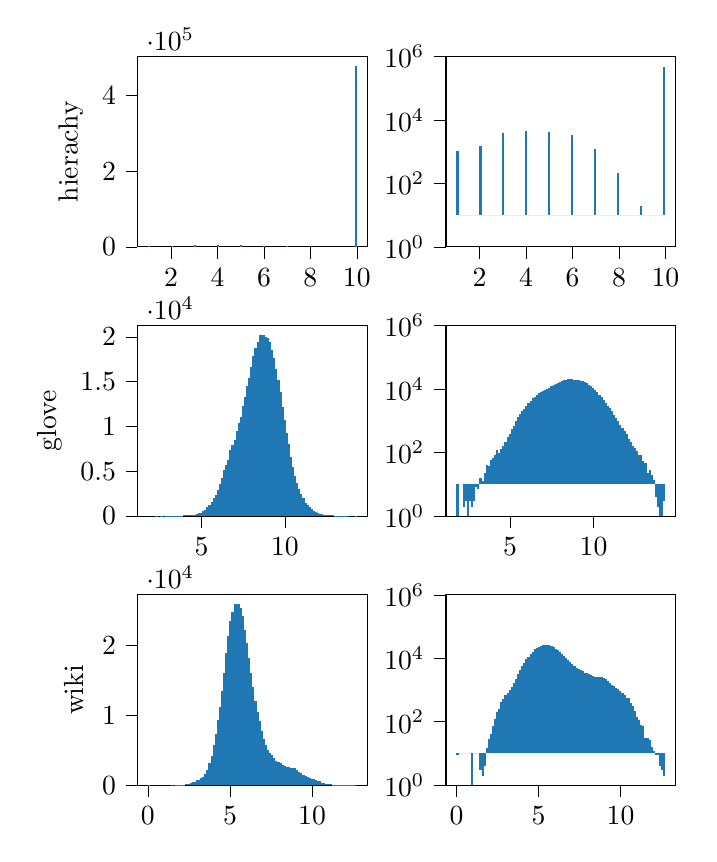
\begin{tikzpicture}

\definecolor{darkgray176}{RGB}{176,176,176}
\definecolor{steelblue31119180}{RGB}{31,119,180}

\begin{groupplot}[group style={group size=2 by 3}]
\nextgroupplot[
height=4cm,
tick align=outside,
tick pos=left,
width=4.5cm,
x grid style={darkgray176},
xmin=0.55, xmax=10.45,
xtick style={color=black},
y grid style={darkgray176},
ylabel={hierachy},
ymin=0, ymax=503696.55,
ytick style={color=black}
]
\draw[draw=none,fill=steelblue31119180] (axis cs:1,0) rectangle (axis cs:1.09,1065);
\draw[draw=none,fill=steelblue31119180] (axis cs:1.09,0) rectangle (axis cs:1.18,0);
\draw[draw=none,fill=steelblue31119180] (axis cs:1.18,0) rectangle (axis cs:1.27,0);
\draw[draw=none,fill=steelblue31119180] (axis cs:1.27,0) rectangle (axis cs:1.36,0);
\draw[draw=none,fill=steelblue31119180] (axis cs:1.36,0) rectangle (axis cs:1.45,0);
\draw[draw=none,fill=steelblue31119180] (axis cs:1.45,0) rectangle (axis cs:1.54,0);
\draw[draw=none,fill=steelblue31119180] (axis cs:1.54,0) rectangle (axis cs:1.63,0);
\draw[draw=none,fill=steelblue31119180] (axis cs:1.63,0) rectangle (axis cs:1.72,0);
\draw[draw=none,fill=steelblue31119180] (axis cs:1.72,0) rectangle (axis cs:1.81,0);
\draw[draw=none,fill=steelblue31119180] (axis cs:1.81,0) rectangle (axis cs:1.9,0);
\draw[draw=none,fill=steelblue31119180] (axis cs:1.9,0) rectangle (axis cs:1.99,0);
\draw[draw=none,fill=steelblue31119180] (axis cs:1.99,0) rectangle (axis cs:2.08,1519);
\draw[draw=none,fill=steelblue31119180] (axis cs:2.08,0) rectangle (axis cs:2.17,0);
\draw[draw=none,fill=steelblue31119180] (axis cs:2.17,0) rectangle (axis cs:2.26,0);
\draw[draw=none,fill=steelblue31119180] (axis cs:2.26,0) rectangle (axis cs:2.35,0);
\draw[draw=none,fill=steelblue31119180] (axis cs:2.35,0) rectangle (axis cs:2.44,0);
\draw[draw=none,fill=steelblue31119180] (axis cs:2.44,0) rectangle (axis cs:2.53,0);
\draw[draw=none,fill=steelblue31119180] (axis cs:2.53,0) rectangle (axis cs:2.62,0);
\draw[draw=none,fill=steelblue31119180] (axis cs:2.62,0) rectangle (axis cs:2.71,0);
\draw[draw=none,fill=steelblue31119180] (axis cs:2.71,0) rectangle (axis cs:2.8,0);
\draw[draw=none,fill=steelblue31119180] (axis cs:2.8,0) rectangle (axis cs:2.89,0);
\draw[draw=none,fill=steelblue31119180] (axis cs:2.89,0) rectangle (axis cs:2.98,0);
\draw[draw=none,fill=steelblue31119180] (axis cs:2.98,0) rectangle (axis cs:3.07,3810);
\draw[draw=none,fill=steelblue31119180] (axis cs:3.07,0) rectangle (axis cs:3.16,0);
\draw[draw=none,fill=steelblue31119180] (axis cs:3.16,0) rectangle (axis cs:3.25,0);
\draw[draw=none,fill=steelblue31119180] (axis cs:3.25,0) rectangle (axis cs:3.34,0);
\draw[draw=none,fill=steelblue31119180] (axis cs:3.34,0) rectangle (axis cs:3.43,0);
\draw[draw=none,fill=steelblue31119180] (axis cs:3.43,0) rectangle (axis cs:3.52,0);
\draw[draw=none,fill=steelblue31119180] (axis cs:3.52,0) rectangle (axis cs:3.61,0);
\draw[draw=none,fill=steelblue31119180] (axis cs:3.61,0) rectangle (axis cs:3.7,0);
\draw[draw=none,fill=steelblue31119180] (axis cs:3.7,0) rectangle (axis cs:3.79,0);
\draw[draw=none,fill=steelblue31119180] (axis cs:3.79,0) rectangle (axis cs:3.88,0);
\draw[draw=none,fill=steelblue31119180] (axis cs:3.88,0) rectangle (axis cs:3.97,0);
\draw[draw=none,fill=steelblue31119180] (axis cs:3.97,0) rectangle (axis cs:4.06,4327);
\draw[draw=none,fill=steelblue31119180] (axis cs:4.06,0) rectangle (axis cs:4.15,0);
\draw[draw=none,fill=steelblue31119180] (axis cs:4.15,0) rectangle (axis cs:4.24,0);
\draw[draw=none,fill=steelblue31119180] (axis cs:4.24,0) rectangle (axis cs:4.33,0);
\draw[draw=none,fill=steelblue31119180] (axis cs:4.33,0) rectangle (axis cs:4.42,0);
\draw[draw=none,fill=steelblue31119180] (axis cs:4.42,0) rectangle (axis cs:4.51,0);
\draw[draw=none,fill=steelblue31119180] (axis cs:4.51,0) rectangle (axis cs:4.6,0);
\draw[draw=none,fill=steelblue31119180] (axis cs:4.6,0) rectangle (axis cs:4.69,0);
\draw[draw=none,fill=steelblue31119180] (axis cs:4.69,0) rectangle (axis cs:4.78,0);
\draw[draw=none,fill=steelblue31119180] (axis cs:4.78,0) rectangle (axis cs:4.87,0);
\draw[draw=none,fill=steelblue31119180] (axis cs:4.87,0) rectangle (axis cs:4.96,0);
\draw[draw=none,fill=steelblue31119180] (axis cs:4.96,0) rectangle (axis cs:5.05,4268);
\draw[draw=none,fill=steelblue31119180] (axis cs:5.05,0) rectangle (axis cs:5.14,0);
\draw[draw=none,fill=steelblue31119180] (axis cs:5.14,0) rectangle (axis cs:5.23,0);
\draw[draw=none,fill=steelblue31119180] (axis cs:5.23,0) rectangle (axis cs:5.32,0);
\draw[draw=none,fill=steelblue31119180] (axis cs:5.32,0) rectangle (axis cs:5.41,0);
\draw[draw=none,fill=steelblue31119180] (axis cs:5.41,0) rectangle (axis cs:5.5,0);
\draw[draw=none,fill=steelblue31119180] (axis cs:5.5,0) rectangle (axis cs:5.59,0);
\draw[draw=none,fill=steelblue31119180] (axis cs:5.59,0) rectangle (axis cs:5.68,0);
\draw[draw=none,fill=steelblue31119180] (axis cs:5.68,0) rectangle (axis cs:5.77,0);
\draw[draw=none,fill=steelblue31119180] (axis cs:5.77,0) rectangle (axis cs:5.86,0);
\draw[draw=none,fill=steelblue31119180] (axis cs:5.86,0) rectangle (axis cs:5.95,0);
\draw[draw=none,fill=steelblue31119180] (axis cs:5.95,0) rectangle (axis cs:6.04,3337);
\draw[draw=none,fill=steelblue31119180] (axis cs:6.04,0) rectangle (axis cs:6.13,0);
\draw[draw=none,fill=steelblue31119180] (axis cs:6.13,0) rectangle (axis cs:6.22,0);
\draw[draw=none,fill=steelblue31119180] (axis cs:6.22,0) rectangle (axis cs:6.31,0);
\draw[draw=none,fill=steelblue31119180] (axis cs:6.31,0) rectangle (axis cs:6.4,0);
\draw[draw=none,fill=steelblue31119180] (axis cs:6.4,0) rectangle (axis cs:6.49,0);
\draw[draw=none,fill=steelblue31119180] (axis cs:6.49,0) rectangle (axis cs:6.58,0);
\draw[draw=none,fill=steelblue31119180] (axis cs:6.58,0) rectangle (axis cs:6.67,0);
\draw[draw=none,fill=steelblue31119180] (axis cs:6.67,0) rectangle (axis cs:6.76,0);
\draw[draw=none,fill=steelblue31119180] (axis cs:6.76,0) rectangle (axis cs:6.85,0);
\draw[draw=none,fill=steelblue31119180] (axis cs:6.85,0) rectangle (axis cs:6.94,0);
\draw[draw=none,fill=steelblue31119180] (axis cs:6.94,0) rectangle (axis cs:7.03,1229);
\draw[draw=none,fill=steelblue31119180] (axis cs:7.03,0) rectangle (axis cs:7.12,0);
\draw[draw=none,fill=steelblue31119180] (axis cs:7.12,0) rectangle (axis cs:7.21,0);
\draw[draw=none,fill=steelblue31119180] (axis cs:7.21,0) rectangle (axis cs:7.3,0);
\draw[draw=none,fill=steelblue31119180] (axis cs:7.3,0) rectangle (axis cs:7.39,0);
\draw[draw=none,fill=steelblue31119180] (axis cs:7.39,0) rectangle (axis cs:7.48,0);
\draw[draw=none,fill=steelblue31119180] (axis cs:7.48,0) rectangle (axis cs:7.57,0);
\draw[draw=none,fill=steelblue31119180] (axis cs:7.57,0) rectangle (axis cs:7.66,0);
\draw[draw=none,fill=steelblue31119180] (axis cs:7.66,0) rectangle (axis cs:7.75,0);
\draw[draw=none,fill=steelblue31119180] (axis cs:7.75,0) rectangle (axis cs:7.84,0);
\draw[draw=none,fill=steelblue31119180] (axis cs:7.84,0) rectangle (axis cs:7.93,0);
\draw[draw=none,fill=steelblue31119180] (axis cs:7.93,0) rectangle (axis cs:8.02,214);
\draw[draw=none,fill=steelblue31119180] (axis cs:8.02,0) rectangle (axis cs:8.11,0);
\draw[draw=none,fill=steelblue31119180] (axis cs:8.11,0) rectangle (axis cs:8.2,0);
\draw[draw=none,fill=steelblue31119180] (axis cs:8.2,0) rectangle (axis cs:8.29,0);
\draw[draw=none,fill=steelblue31119180] (axis cs:8.29,0) rectangle (axis cs:8.38,0);
\draw[draw=none,fill=steelblue31119180] (axis cs:8.38,0) rectangle (axis cs:8.47,0);
\draw[draw=none,fill=steelblue31119180] (axis cs:8.47,0) rectangle (axis cs:8.56,0);
\draw[draw=none,fill=steelblue31119180] (axis cs:8.56,0) rectangle (axis cs:8.65,0);
\draw[draw=none,fill=steelblue31119180] (axis cs:8.65,0) rectangle (axis cs:8.74,0);
\draw[draw=none,fill=steelblue31119180] (axis cs:8.74,0) rectangle (axis cs:8.83,0);
\draw[draw=none,fill=steelblue31119180] (axis cs:8.83,0) rectangle (axis cs:8.92,0);
\draw[draw=none,fill=steelblue31119180] (axis cs:8.92,0) rectangle (axis cs:9.01,20);
\draw[draw=none,fill=steelblue31119180] (axis cs:9.01,0) rectangle (axis cs:9.1,0);
\draw[draw=none,fill=steelblue31119180] (axis cs:9.1,0) rectangle (axis cs:9.19,0);
\draw[draw=none,fill=steelblue31119180] (axis cs:9.19,0) rectangle (axis cs:9.28,0);
\draw[draw=none,fill=steelblue31119180] (axis cs:9.28,0) rectangle (axis cs:9.37,0);
\draw[draw=none,fill=steelblue31119180] (axis cs:9.37,0) rectangle (axis cs:9.46,0);
\draw[draw=none,fill=steelblue31119180] (axis cs:9.46,0) rectangle (axis cs:9.55,0);
\draw[draw=none,fill=steelblue31119180] (axis cs:9.55,0) rectangle (axis cs:9.64,0);
\draw[draw=none,fill=steelblue31119180] (axis cs:9.64,0) rectangle (axis cs:9.73,0);
\draw[draw=none,fill=steelblue31119180] (axis cs:9.73,0) rectangle (axis cs:9.82,0);
\draw[draw=none,fill=steelblue31119180] (axis cs:9.82,0) rectangle (axis cs:9.91,0);
\draw[draw=none,fill=steelblue31119180] (axis cs:9.91,0) rectangle (axis cs:10,479711);

\nextgroupplot[
height=4cm,
log basis y={10},
tick align=outside,
tick pos=left,
width=4.5cm,
x grid style={darkgray176},
xmin=0.55, xmax=10.45,
xtick style={color=black},
y grid style={darkgray176},
ymin=1, ymax=1000000,
ymode=log,
ytick style={color=black}
]
\draw[draw=none,fill=steelblue31119180] (axis cs:1,0) rectangle (axis cs:1.09,1065);
\draw[draw=none,fill=steelblue31119180] (axis cs:1.09,0) rectangle (axis cs:1.18,0);
\draw[draw=none,fill=steelblue31119180] (axis cs:1.18,0) rectangle (axis cs:1.27,0);
\draw[draw=none,fill=steelblue31119180] (axis cs:1.27,0) rectangle (axis cs:1.36,0);
\draw[draw=none,fill=steelblue31119180] (axis cs:1.36,0) rectangle (axis cs:1.45,0);
\draw[draw=none,fill=steelblue31119180] (axis cs:1.45,0) rectangle (axis cs:1.54,0);
\draw[draw=none,fill=steelblue31119180] (axis cs:1.54,0) rectangle (axis cs:1.63,0);
\draw[draw=none,fill=steelblue31119180] (axis cs:1.63,0) rectangle (axis cs:1.72,0);
\draw[draw=none,fill=steelblue31119180] (axis cs:1.72,0) rectangle (axis cs:1.81,0);
\draw[draw=none,fill=steelblue31119180] (axis cs:1.81,0) rectangle (axis cs:1.9,0);
\draw[draw=none,fill=steelblue31119180] (axis cs:1.9,0) rectangle (axis cs:1.99,0);
\draw[draw=none,fill=steelblue31119180] (axis cs:1.99,0) rectangle (axis cs:2.08,1519);
\draw[draw=none,fill=steelblue31119180] (axis cs:2.08,0) rectangle (axis cs:2.17,0);
\draw[draw=none,fill=steelblue31119180] (axis cs:2.17,0) rectangle (axis cs:2.26,0);
\draw[draw=none,fill=steelblue31119180] (axis cs:2.26,0) rectangle (axis cs:2.35,0);
\draw[draw=none,fill=steelblue31119180] (axis cs:2.35,0) rectangle (axis cs:2.44,0);
\draw[draw=none,fill=steelblue31119180] (axis cs:2.44,0) rectangle (axis cs:2.53,0);
\draw[draw=none,fill=steelblue31119180] (axis cs:2.53,0) rectangle (axis cs:2.62,0);
\draw[draw=none,fill=steelblue31119180] (axis cs:2.62,0) rectangle (axis cs:2.71,0);
\draw[draw=none,fill=steelblue31119180] (axis cs:2.71,0) rectangle (axis cs:2.8,0);
\draw[draw=none,fill=steelblue31119180] (axis cs:2.8,0) rectangle (axis cs:2.89,0);
\draw[draw=none,fill=steelblue31119180] (axis cs:2.89,0) rectangle (axis cs:2.98,0);
\draw[draw=none,fill=steelblue31119180] (axis cs:2.98,0) rectangle (axis cs:3.07,3810);
\draw[draw=none,fill=steelblue31119180] (axis cs:3.07,0) rectangle (axis cs:3.16,0);
\draw[draw=none,fill=steelblue31119180] (axis cs:3.16,0) rectangle (axis cs:3.25,0);
\draw[draw=none,fill=steelblue31119180] (axis cs:3.25,0) rectangle (axis cs:3.34,0);
\draw[draw=none,fill=steelblue31119180] (axis cs:3.34,0) rectangle (axis cs:3.43,0);
\draw[draw=none,fill=steelblue31119180] (axis cs:3.43,0) rectangle (axis cs:3.52,0);
\draw[draw=none,fill=steelblue31119180] (axis cs:3.52,0) rectangle (axis cs:3.61,0);
\draw[draw=none,fill=steelblue31119180] (axis cs:3.61,0) rectangle (axis cs:3.7,0);
\draw[draw=none,fill=steelblue31119180] (axis cs:3.7,0) rectangle (axis cs:3.79,0);
\draw[draw=none,fill=steelblue31119180] (axis cs:3.79,0) rectangle (axis cs:3.88,0);
\draw[draw=none,fill=steelblue31119180] (axis cs:3.88,0) rectangle (axis cs:3.97,0);
\draw[draw=none,fill=steelblue31119180] (axis cs:3.97,0) rectangle (axis cs:4.06,4327);
\draw[draw=none,fill=steelblue31119180] (axis cs:4.06,0) rectangle (axis cs:4.15,0);
\draw[draw=none,fill=steelblue31119180] (axis cs:4.15,0) rectangle (axis cs:4.24,0);
\draw[draw=none,fill=steelblue31119180] (axis cs:4.24,0) rectangle (axis cs:4.33,0);
\draw[draw=none,fill=steelblue31119180] (axis cs:4.33,0) rectangle (axis cs:4.42,0);
\draw[draw=none,fill=steelblue31119180] (axis cs:4.42,0) rectangle (axis cs:4.51,0);
\draw[draw=none,fill=steelblue31119180] (axis cs:4.51,0) rectangle (axis cs:4.6,0);
\draw[draw=none,fill=steelblue31119180] (axis cs:4.6,0) rectangle (axis cs:4.69,0);
\draw[draw=none,fill=steelblue31119180] (axis cs:4.69,0) rectangle (axis cs:4.78,0);
\draw[draw=none,fill=steelblue31119180] (axis cs:4.78,0) rectangle (axis cs:4.87,0);
\draw[draw=none,fill=steelblue31119180] (axis cs:4.87,0) rectangle (axis cs:4.96,0);
\draw[draw=none,fill=steelblue31119180] (axis cs:4.96,0) rectangle (axis cs:5.05,4268);
\draw[draw=none,fill=steelblue31119180] (axis cs:5.05,0) rectangle (axis cs:5.14,0);
\draw[draw=none,fill=steelblue31119180] (axis cs:5.14,0) rectangle (axis cs:5.23,0);
\draw[draw=none,fill=steelblue31119180] (axis cs:5.23,0) rectangle (axis cs:5.32,0);
\draw[draw=none,fill=steelblue31119180] (axis cs:5.32,0) rectangle (axis cs:5.41,0);
\draw[draw=none,fill=steelblue31119180] (axis cs:5.41,0) rectangle (axis cs:5.5,0);
\draw[draw=none,fill=steelblue31119180] (axis cs:5.5,0) rectangle (axis cs:5.59,0);
\draw[draw=none,fill=steelblue31119180] (axis cs:5.59,0) rectangle (axis cs:5.68,0);
\draw[draw=none,fill=steelblue31119180] (axis cs:5.68,0) rectangle (axis cs:5.77,0);
\draw[draw=none,fill=steelblue31119180] (axis cs:5.77,0) rectangle (axis cs:5.86,0);
\draw[draw=none,fill=steelblue31119180] (axis cs:5.86,0) rectangle (axis cs:5.95,0);
\draw[draw=none,fill=steelblue31119180] (axis cs:5.95,0) rectangle (axis cs:6.04,3337);
\draw[draw=none,fill=steelblue31119180] (axis cs:6.04,0) rectangle (axis cs:6.13,0);
\draw[draw=none,fill=steelblue31119180] (axis cs:6.13,0) rectangle (axis cs:6.22,0);
\draw[draw=none,fill=steelblue31119180] (axis cs:6.22,0) rectangle (axis cs:6.31,0);
\draw[draw=none,fill=steelblue31119180] (axis cs:6.31,0) rectangle (axis cs:6.4,0);
\draw[draw=none,fill=steelblue31119180] (axis cs:6.4,0) rectangle (axis cs:6.49,0);
\draw[draw=none,fill=steelblue31119180] (axis cs:6.49,0) rectangle (axis cs:6.58,0);
\draw[draw=none,fill=steelblue31119180] (axis cs:6.58,0) rectangle (axis cs:6.67,0);
\draw[draw=none,fill=steelblue31119180] (axis cs:6.67,0) rectangle (axis cs:6.76,0);
\draw[draw=none,fill=steelblue31119180] (axis cs:6.76,0) rectangle (axis cs:6.85,0);
\draw[draw=none,fill=steelblue31119180] (axis cs:6.85,0) rectangle (axis cs:6.94,0);
\draw[draw=none,fill=steelblue31119180] (axis cs:6.94,0) rectangle (axis cs:7.03,1229);
\draw[draw=none,fill=steelblue31119180] (axis cs:7.03,0) rectangle (axis cs:7.12,0);
\draw[draw=none,fill=steelblue31119180] (axis cs:7.12,0) rectangle (axis cs:7.21,0);
\draw[draw=none,fill=steelblue31119180] (axis cs:7.21,0) rectangle (axis cs:7.3,0);
\draw[draw=none,fill=steelblue31119180] (axis cs:7.3,0) rectangle (axis cs:7.39,0);
\draw[draw=none,fill=steelblue31119180] (axis cs:7.39,0) rectangle (axis cs:7.48,0);
\draw[draw=none,fill=steelblue31119180] (axis cs:7.48,0) rectangle (axis cs:7.57,0);
\draw[draw=none,fill=steelblue31119180] (axis cs:7.57,0) rectangle (axis cs:7.66,0);
\draw[draw=none,fill=steelblue31119180] (axis cs:7.66,0) rectangle (axis cs:7.75,0);
\draw[draw=none,fill=steelblue31119180] (axis cs:7.75,0) rectangle (axis cs:7.84,0);
\draw[draw=none,fill=steelblue31119180] (axis cs:7.84,0) rectangle (axis cs:7.93,0);
\draw[draw=none,fill=steelblue31119180] (axis cs:7.93,0) rectangle (axis cs:8.02,214);
\draw[draw=none,fill=steelblue31119180] (axis cs:8.02,0) rectangle (axis cs:8.11,0);
\draw[draw=none,fill=steelblue31119180] (axis cs:8.11,0) rectangle (axis cs:8.2,0);
\draw[draw=none,fill=steelblue31119180] (axis cs:8.2,0) rectangle (axis cs:8.29,0);
\draw[draw=none,fill=steelblue31119180] (axis cs:8.29,0) rectangle (axis cs:8.38,0);
\draw[draw=none,fill=steelblue31119180] (axis cs:8.38,0) rectangle (axis cs:8.47,0);
\draw[draw=none,fill=steelblue31119180] (axis cs:8.47,0) rectangle (axis cs:8.56,0);
\draw[draw=none,fill=steelblue31119180] (axis cs:8.56,0) rectangle (axis cs:8.65,0);
\draw[draw=none,fill=steelblue31119180] (axis cs:8.65,0) rectangle (axis cs:8.74,0);
\draw[draw=none,fill=steelblue31119180] (axis cs:8.74,0) rectangle (axis cs:8.83,0);
\draw[draw=none,fill=steelblue31119180] (axis cs:8.83,0) rectangle (axis cs:8.92,0);
\draw[draw=none,fill=steelblue31119180] (axis cs:8.92,0) rectangle (axis cs:9.01,20);
\draw[draw=none,fill=steelblue31119180] (axis cs:9.01,0) rectangle (axis cs:9.1,0);
\draw[draw=none,fill=steelblue31119180] (axis cs:9.1,0) rectangle (axis cs:9.19,0);
\draw[draw=none,fill=steelblue31119180] (axis cs:9.19,0) rectangle (axis cs:9.28,0);
\draw[draw=none,fill=steelblue31119180] (axis cs:9.28,0) rectangle (axis cs:9.37,0);
\draw[draw=none,fill=steelblue31119180] (axis cs:9.37,0) rectangle (axis cs:9.46,0);
\draw[draw=none,fill=steelblue31119180] (axis cs:9.46,0) rectangle (axis cs:9.55,0);
\draw[draw=none,fill=steelblue31119180] (axis cs:9.55,0) rectangle (axis cs:9.64,0);
\draw[draw=none,fill=steelblue31119180] (axis cs:9.64,0) rectangle (axis cs:9.73,0);
\draw[draw=none,fill=steelblue31119180] (axis cs:9.73,0) rectangle (axis cs:9.82,0);
\draw[draw=none,fill=steelblue31119180] (axis cs:9.82,0) rectangle (axis cs:9.91,0);
\draw[draw=none,fill=steelblue31119180] (axis cs:9.91,0) rectangle (axis cs:10,479711);

\nextgroupplot[
height=4cm,
tick align=outside,
tick pos=left,
width=4.5cm,
x grid style={darkgray176},
xmin=1.15033604865731, xmax=14.9357449579122,
xtick style={color=black},
y grid style={darkgray176},
ylabel={glove},
ymin=0, ymax=21262.5,
ytick style={color=black}
]
\draw[draw=none,fill=steelblue31119180] (axis cs:1.77694554453253,0) rectangle (axis cs:1.90226744370758,1);
\draw[draw=none,fill=steelblue31119180] (axis cs:1.90226744370758,0) rectangle (axis cs:2.02758934288262,0);
\draw[draw=none,fill=steelblue31119180] (axis cs:2.02758934288262,0) rectangle (axis cs:2.15291124205766,0);
\draw[draw=none,fill=steelblue31119180] (axis cs:2.15291124205766,0) rectangle (axis cs:2.27823314123271,2);
\draw[draw=none,fill=steelblue31119180] (axis cs:2.27823314123271,0) rectangle (axis cs:2.40355504040775,3);
\draw[draw=none,fill=steelblue31119180] (axis cs:2.40355504040775,0) rectangle (axis cs:2.5288769395828,1);
\draw[draw=none,fill=steelblue31119180] (axis cs:2.5288769395828,0) rectangle (axis cs:2.65419883875784,3);
\draw[draw=none,fill=steelblue31119180] (axis cs:2.65419883875784,0) rectangle (axis cs:2.77952073793288,2);
\draw[draw=none,fill=steelblue31119180] (axis cs:2.77952073793288,0) rectangle (axis cs:2.90484263710793,3);
\draw[draw=none,fill=steelblue31119180] (axis cs:2.90484263710793,0) rectangle (axis cs:3.03016453628297,8);
\draw[draw=none,fill=steelblue31119180] (axis cs:3.03016453628297,0) rectangle (axis cs:3.15548643545802,7);
\draw[draw=none,fill=steelblue31119180] (axis cs:3.15548643545802,0) rectangle (axis cs:3.28080833463306,16);
\draw[draw=none,fill=steelblue31119180] (axis cs:3.28080833463306,0) rectangle (axis cs:3.4061302338081,13);
\draw[draw=none,fill=steelblue31119180] (axis cs:3.4061302338081,0) rectangle (axis cs:3.53145213298315,22);
\draw[draw=none,fill=steelblue31119180] (axis cs:3.53145213298315,0) rectangle (axis cs:3.65677403215819,42);
\draw[draw=none,fill=steelblue31119180] (axis cs:3.65677403215819,0) rectangle (axis cs:3.78209593133324,39);
\draw[draw=none,fill=steelblue31119180] (axis cs:3.78209593133324,0) rectangle (axis cs:3.90741783050828,60);
\draw[draw=none,fill=steelblue31119180] (axis cs:3.90741783050828,0) rectangle (axis cs:4.03273972968332,68);
\draw[draw=none,fill=steelblue31119180] (axis cs:4.03273972968332,0) rectangle (axis cs:4.15806162885837,83);
\draw[draw=none,fill=steelblue31119180] (axis cs:4.15806162885837,0) rectangle (axis cs:4.28338352803341,118);
\draw[draw=none,fill=steelblue31119180] (axis cs:4.28338352803341,0) rectangle (axis cs:4.40870542720846,98);
\draw[draw=none,fill=steelblue31119180] (axis cs:4.40870542720846,0) rectangle (axis cs:4.5340273263835,134);
\draw[draw=none,fill=steelblue31119180] (axis cs:4.5340273263835,0) rectangle (axis cs:4.65934922555854,165);
\draw[draw=none,fill=steelblue31119180] (axis cs:4.65934922555854,0) rectangle (axis cs:4.78467112473359,222);
\draw[draw=none,fill=steelblue31119180] (axis cs:4.78467112473359,0) rectangle (axis cs:4.90999302390863,309);
\draw[draw=none,fill=steelblue31119180] (axis cs:4.90999302390863,0) rectangle (axis cs:5.03531492308368,395);
\draw[draw=none,fill=steelblue31119180] (axis cs:5.03531492308368,0) rectangle (axis cs:5.16063682225872,569);
\draw[draw=none,fill=steelblue31119180] (axis cs:5.16063682225872,0) rectangle (axis cs:5.28595872143377,710);
\draw[draw=none,fill=steelblue31119180] (axis cs:5.28595872143377,0) rectangle (axis cs:5.41128062060881,1013);
\draw[draw=none,fill=steelblue31119180] (axis cs:5.41128062060881,0) rectangle (axis cs:5.53660251978385,1281);
\draw[draw=none,fill=steelblue31119180] (axis cs:5.53660251978385,0) rectangle (axis cs:5.6619244189589,1612);
\draw[draw=none,fill=steelblue31119180] (axis cs:5.6619244189589,0) rectangle (axis cs:5.78724631813394,2043);
\draw[draw=none,fill=steelblue31119180] (axis cs:5.78724631813394,0) rectangle (axis cs:5.91256821730899,2404);
\draw[draw=none,fill=steelblue31119180] (axis cs:5.91256821730899,0) rectangle (axis cs:6.03789011648403,2951);
\draw[draw=none,fill=steelblue31119180] (axis cs:6.03789011648403,0) rectangle (axis cs:6.16321201565908,3619);
\draw[draw=none,fill=steelblue31119180] (axis cs:6.16321201565908,0) rectangle (axis cs:6.28853391483412,4252);
\draw[draw=none,fill=steelblue31119180] (axis cs:6.28853391483412,0) rectangle (axis cs:6.41385581400916,5100);
\draw[draw=none,fill=steelblue31119180] (axis cs:6.41385581400916,0) rectangle (axis cs:6.53917771318421,5691);
\draw[draw=none,fill=steelblue31119180] (axis cs:6.53917771318421,0) rectangle (axis cs:6.66449961235925,6301);
\draw[draw=none,fill=steelblue31119180] (axis cs:6.66449961235925,0) rectangle (axis cs:6.7898215115343,7410);
\draw[draw=none,fill=steelblue31119180] (axis cs:6.7898215115343,0) rectangle (axis cs:6.91514341070934,7910);
\draw[draw=none,fill=steelblue31119180] (axis cs:6.91514341070934,0) rectangle (axis cs:7.04046530988438,8519);
\draw[draw=none,fill=steelblue31119180] (axis cs:7.04046530988438,0) rectangle (axis cs:7.16578720905943,9491);
\draw[draw=none,fill=steelblue31119180] (axis cs:7.16578720905943,0) rectangle (axis cs:7.29110910823447,10412);
\draw[draw=none,fill=steelblue31119180] (axis cs:7.29110910823447,0) rectangle (axis cs:7.41643100740952,11049);
\draw[draw=none,fill=steelblue31119180] (axis cs:7.41643100740952,0) rectangle (axis cs:7.54175290658456,12272);
\draw[draw=none,fill=steelblue31119180] (axis cs:7.54175290658456,0) rectangle (axis cs:7.6670748057596,13317);
\draw[draw=none,fill=steelblue31119180] (axis cs:7.6670748057596,0) rectangle (axis cs:7.79239670493465,14538);
\draw[draw=none,fill=steelblue31119180] (axis cs:7.79239670493465,0) rectangle (axis cs:7.91771860410969,15398);
\draw[draw=none,fill=steelblue31119180] (axis cs:7.91771860410969,0) rectangle (axis cs:8.04304050328474,16695);
\draw[draw=none,fill=steelblue31119180] (axis cs:8.04304050328474,0) rectangle (axis cs:8.16836240245978,17887);
\draw[draw=none,fill=steelblue31119180] (axis cs:8.16836240245978,0) rectangle (axis cs:8.29368430163482,18769);
\draw[draw=none,fill=steelblue31119180] (axis cs:8.29368430163483,0) rectangle (axis cs:8.41900620080987,19457);
\draw[draw=none,fill=steelblue31119180] (axis cs:8.41900620080987,0) rectangle (axis cs:8.54432809998491,20208);
\draw[draw=none,fill=steelblue31119180] (axis cs:8.54432809998491,0) rectangle (axis cs:8.66964999915996,20197);
\draw[draw=none,fill=steelblue31119180] (axis cs:8.66964999915996,0) rectangle (axis cs:8.794971898335,20250);
\draw[draw=none,fill=steelblue31119180] (axis cs:8.794971898335,0) rectangle (axis cs:8.92029379751005,20041);
\draw[draw=none,fill=steelblue31119180] (axis cs:8.92029379751004,0) rectangle (axis cs:9.04561569668509,19929);
\draw[draw=none,fill=steelblue31119180] (axis cs:9.04561569668509,0) rectangle (axis cs:9.17093759586013,19486);
\draw[draw=none,fill=steelblue31119180] (axis cs:9.17093759586013,0) rectangle (axis cs:9.29625949503518,18535);
\draw[draw=none,fill=steelblue31119180] (axis cs:9.29625949503518,0) rectangle (axis cs:9.42158139421022,17680);
\draw[draw=none,fill=steelblue31119180] (axis cs:9.42158139421022,0) rectangle (axis cs:9.54690329338526,16464);
\draw[draw=none,fill=steelblue31119180] (axis cs:9.54690329338526,0) rectangle (axis cs:9.67222519256031,15153);
\draw[draw=none,fill=steelblue31119180] (axis cs:9.67222519256031,0) rectangle (axis cs:9.79754709173536,13891);
\draw[draw=none,fill=steelblue31119180] (axis cs:9.79754709173535,0) rectangle (axis cs:9.9228689909104,12150);
\draw[draw=none,fill=steelblue31119180] (axis cs:9.9228689909104,0) rectangle (axis cs:10.0481908900854,10726);
\draw[draw=none,fill=steelblue31119180] (axis cs:10.0481908900854,0) rectangle (axis cs:10.1735127892605,9231);
\draw[draw=none,fill=steelblue31119180] (axis cs:10.1735127892605,0) rectangle (axis cs:10.2988346884355,8067);
\draw[draw=none,fill=steelblue31119180] (axis cs:10.2988346884355,0) rectangle (axis cs:10.4241565876106,6647);
\draw[draw=none,fill=steelblue31119180] (axis cs:10.4241565876106,0) rectangle (axis cs:10.5494784867856,5472);
\draw[draw=none,fill=steelblue31119180] (axis cs:10.5494784867856,0) rectangle (axis cs:10.6748003859607,4478);
\draw[draw=none,fill=steelblue31119180] (axis cs:10.6748003859607,0) rectangle (axis cs:10.8001222851357,3706);
\draw[draw=none,fill=steelblue31119180] (axis cs:10.8001222851357,0) rectangle (axis cs:10.9254441843108,2993);
\draw[draw=none,fill=steelblue31119180] (axis cs:10.9254441843108,0) rectangle (axis cs:11.0507660834858,2480);
\draw[draw=none,fill=steelblue31119180] (axis cs:11.0507660834858,0) rectangle (axis cs:11.1760879826608,2012);
\draw[draw=none,fill=steelblue31119180] (axis cs:11.1760879826608,0) rectangle (axis cs:11.3014098818359,1480);
\draw[draw=none,fill=steelblue31119180] (axis cs:11.3014098818359,0) rectangle (axis cs:11.4267317810109,1256);
\draw[draw=none,fill=steelblue31119180] (axis cs:11.4267317810109,0) rectangle (axis cs:11.552053680186,975);
\draw[draw=none,fill=steelblue31119180] (axis cs:11.552053680186,0) rectangle (axis cs:11.677375579361,756);
\draw[draw=none,fill=steelblue31119180] (axis cs:11.677375579361,0) rectangle (axis cs:11.8026974785361,601);
\draw[draw=none,fill=steelblue31119180] (axis cs:11.8026974785361,0) rectangle (axis cs:11.9280193777111,485);
\draw[draw=none,fill=steelblue31119180] (axis cs:11.9280193777111,0) rectangle (axis cs:12.0533412768861,396);
\draw[draw=none,fill=steelblue31119180] (axis cs:12.0533412768861,0) rectangle (axis cs:12.1786631760612,268);
\draw[draw=none,fill=steelblue31119180] (axis cs:12.1786631760612,0) rectangle (axis cs:12.3039850752362,217);
\draw[draw=none,fill=steelblue31119180] (axis cs:12.3039850752362,0) rectangle (axis cs:12.4293069744113,166);
\draw[draw=none,fill=steelblue31119180] (axis cs:12.4293069744113,0) rectangle (axis cs:12.5546288735863,140);
\draw[draw=none,fill=steelblue31119180] (axis cs:12.5546288735863,0) rectangle (axis cs:12.6799507727614,116);
\draw[draw=none,fill=steelblue31119180] (axis cs:12.6799507727614,0) rectangle (axis cs:12.8052726719364,83);
\draw[draw=none,fill=steelblue31119180] (axis cs:12.8052726719364,0) rectangle (axis cs:12.9305945711115,82);
\draw[draw=none,fill=steelblue31119180] (axis cs:12.9305945711115,0) rectangle (axis cs:13.0559164702865,54);
\draw[draw=none,fill=steelblue31119180] (axis cs:13.0559164702865,0) rectangle (axis cs:13.1812383694615,46);
\draw[draw=none,fill=steelblue31119180] (axis cs:13.1812383694615,0) rectangle (axis cs:13.3065602686366,23);
\draw[draw=none,fill=steelblue31119180] (axis cs:13.3065602686366,0) rectangle (axis cs:13.4318821678116,29);
\draw[draw=none,fill=steelblue31119180] (axis cs:13.4318821678116,0) rectangle (axis cs:13.5572040669867,20);
\draw[draw=none,fill=steelblue31119180] (axis cs:13.5572040669867,0) rectangle (axis cs:13.6825259661617,14);
\draw[draw=none,fill=steelblue31119180] (axis cs:13.6825259661617,0) rectangle (axis cs:13.8078478653368,4);
\draw[draw=none,fill=steelblue31119180] (axis cs:13.8078478653368,0) rectangle (axis cs:13.9331697645118,2);
\draw[draw=none,fill=steelblue31119180] (axis cs:13.9331697645118,0) rectangle (axis cs:14.0584916636869,1);
\draw[draw=none,fill=steelblue31119180] (axis cs:14.0584916636869,0) rectangle (axis cs:14.1838135628619,1);
\draw[draw=none,fill=steelblue31119180] (axis cs:14.1838135628619,0) rectangle (axis cs:14.3091354620369,3);

\nextgroupplot[
height=4cm,
log basis y={10},
tick align=outside,
tick pos=left,
width=4.5cm,
x grid style={darkgray176},
xmin=1.15033604865731, xmax=14.9357449579122,
xtick style={color=black},
y grid style={darkgray176},
ymin=1, ymax=1000000,
ymode=log,
ytick style={color=black}
]
\draw[draw=none,fill=steelblue31119180] (axis cs:1.77694554453253,0) rectangle (axis cs:1.90226744370758,1);
\draw[draw=none,fill=steelblue31119180] (axis cs:1.90226744370758,0) rectangle (axis cs:2.02758934288262,0);
\draw[draw=none,fill=steelblue31119180] (axis cs:2.02758934288262,0) rectangle (axis cs:2.15291124205766,0);
\draw[draw=none,fill=steelblue31119180] (axis cs:2.15291124205766,0) rectangle (axis cs:2.27823314123271,2);
\draw[draw=none,fill=steelblue31119180] (axis cs:2.27823314123271,0) rectangle (axis cs:2.40355504040775,3);
\draw[draw=none,fill=steelblue31119180] (axis cs:2.40355504040775,0) rectangle (axis cs:2.5288769395828,1);
\draw[draw=none,fill=steelblue31119180] (axis cs:2.5288769395828,0) rectangle (axis cs:2.65419883875784,3);
\draw[draw=none,fill=steelblue31119180] (axis cs:2.65419883875784,0) rectangle (axis cs:2.77952073793288,2);
\draw[draw=none,fill=steelblue31119180] (axis cs:2.77952073793288,0) rectangle (axis cs:2.90484263710793,3);
\draw[draw=none,fill=steelblue31119180] (axis cs:2.90484263710793,0) rectangle (axis cs:3.03016453628297,8);
\draw[draw=none,fill=steelblue31119180] (axis cs:3.03016453628297,0) rectangle (axis cs:3.15548643545802,7);
\draw[draw=none,fill=steelblue31119180] (axis cs:3.15548643545802,0) rectangle (axis cs:3.28080833463306,16);
\draw[draw=none,fill=steelblue31119180] (axis cs:3.28080833463306,0) rectangle (axis cs:3.4061302338081,13);
\draw[draw=none,fill=steelblue31119180] (axis cs:3.4061302338081,0) rectangle (axis cs:3.53145213298315,22);
\draw[draw=none,fill=steelblue31119180] (axis cs:3.53145213298315,0) rectangle (axis cs:3.65677403215819,42);
\draw[draw=none,fill=steelblue31119180] (axis cs:3.65677403215819,0) rectangle (axis cs:3.78209593133324,39);
\draw[draw=none,fill=steelblue31119180] (axis cs:3.78209593133324,0) rectangle (axis cs:3.90741783050828,60);
\draw[draw=none,fill=steelblue31119180] (axis cs:3.90741783050828,0) rectangle (axis cs:4.03273972968332,68);
\draw[draw=none,fill=steelblue31119180] (axis cs:4.03273972968332,0) rectangle (axis cs:4.15806162885837,83);
\draw[draw=none,fill=steelblue31119180] (axis cs:4.15806162885837,0) rectangle (axis cs:4.28338352803341,118);
\draw[draw=none,fill=steelblue31119180] (axis cs:4.28338352803341,0) rectangle (axis cs:4.40870542720846,98);
\draw[draw=none,fill=steelblue31119180] (axis cs:4.40870542720846,0) rectangle (axis cs:4.5340273263835,134);
\draw[draw=none,fill=steelblue31119180] (axis cs:4.5340273263835,0) rectangle (axis cs:4.65934922555854,165);
\draw[draw=none,fill=steelblue31119180] (axis cs:4.65934922555854,0) rectangle (axis cs:4.78467112473359,222);
\draw[draw=none,fill=steelblue31119180] (axis cs:4.78467112473359,0) rectangle (axis cs:4.90999302390863,309);
\draw[draw=none,fill=steelblue31119180] (axis cs:4.90999302390863,0) rectangle (axis cs:5.03531492308368,395);
\draw[draw=none,fill=steelblue31119180] (axis cs:5.03531492308368,0) rectangle (axis cs:5.16063682225872,569);
\draw[draw=none,fill=steelblue31119180] (axis cs:5.16063682225872,0) rectangle (axis cs:5.28595872143377,710);
\draw[draw=none,fill=steelblue31119180] (axis cs:5.28595872143377,0) rectangle (axis cs:5.41128062060881,1013);
\draw[draw=none,fill=steelblue31119180] (axis cs:5.41128062060881,0) rectangle (axis cs:5.53660251978385,1281);
\draw[draw=none,fill=steelblue31119180] (axis cs:5.53660251978385,0) rectangle (axis cs:5.6619244189589,1612);
\draw[draw=none,fill=steelblue31119180] (axis cs:5.6619244189589,0) rectangle (axis cs:5.78724631813394,2043);
\draw[draw=none,fill=steelblue31119180] (axis cs:5.78724631813394,0) rectangle (axis cs:5.91256821730899,2404);
\draw[draw=none,fill=steelblue31119180] (axis cs:5.91256821730899,0) rectangle (axis cs:6.03789011648403,2951);
\draw[draw=none,fill=steelblue31119180] (axis cs:6.03789011648403,0) rectangle (axis cs:6.16321201565908,3619);
\draw[draw=none,fill=steelblue31119180] (axis cs:6.16321201565908,0) rectangle (axis cs:6.28853391483412,4252);
\draw[draw=none,fill=steelblue31119180] (axis cs:6.28853391483412,0) rectangle (axis cs:6.41385581400916,5100);
\draw[draw=none,fill=steelblue31119180] (axis cs:6.41385581400916,0) rectangle (axis cs:6.53917771318421,5691);
\draw[draw=none,fill=steelblue31119180] (axis cs:6.53917771318421,0) rectangle (axis cs:6.66449961235925,6301);
\draw[draw=none,fill=steelblue31119180] (axis cs:6.66449961235925,0) rectangle (axis cs:6.7898215115343,7410);
\draw[draw=none,fill=steelblue31119180] (axis cs:6.7898215115343,0) rectangle (axis cs:6.91514341070934,7910);
\draw[draw=none,fill=steelblue31119180] (axis cs:6.91514341070934,0) rectangle (axis cs:7.04046530988438,8519);
\draw[draw=none,fill=steelblue31119180] (axis cs:7.04046530988438,0) rectangle (axis cs:7.16578720905943,9491);
\draw[draw=none,fill=steelblue31119180] (axis cs:7.16578720905943,0) rectangle (axis cs:7.29110910823447,10412);
\draw[draw=none,fill=steelblue31119180] (axis cs:7.29110910823447,0) rectangle (axis cs:7.41643100740952,11049);
\draw[draw=none,fill=steelblue31119180] (axis cs:7.41643100740952,0) rectangle (axis cs:7.54175290658456,12272);
\draw[draw=none,fill=steelblue31119180] (axis cs:7.54175290658456,0) rectangle (axis cs:7.6670748057596,13317);
\draw[draw=none,fill=steelblue31119180] (axis cs:7.6670748057596,0) rectangle (axis cs:7.79239670493465,14538);
\draw[draw=none,fill=steelblue31119180] (axis cs:7.79239670493465,0) rectangle (axis cs:7.91771860410969,15398);
\draw[draw=none,fill=steelblue31119180] (axis cs:7.91771860410969,0) rectangle (axis cs:8.04304050328474,16695);
\draw[draw=none,fill=steelblue31119180] (axis cs:8.04304050328474,0) rectangle (axis cs:8.16836240245978,17887);
\draw[draw=none,fill=steelblue31119180] (axis cs:8.16836240245978,0) rectangle (axis cs:8.29368430163482,18769);
\draw[draw=none,fill=steelblue31119180] (axis cs:8.29368430163483,0) rectangle (axis cs:8.41900620080987,19457);
\draw[draw=none,fill=steelblue31119180] (axis cs:8.41900620080987,0) rectangle (axis cs:8.54432809998491,20208);
\draw[draw=none,fill=steelblue31119180] (axis cs:8.54432809998491,0) rectangle (axis cs:8.66964999915996,20197);
\draw[draw=none,fill=steelblue31119180] (axis cs:8.66964999915996,0) rectangle (axis cs:8.794971898335,20250);
\draw[draw=none,fill=steelblue31119180] (axis cs:8.794971898335,0) rectangle (axis cs:8.92029379751005,20041);
\draw[draw=none,fill=steelblue31119180] (axis cs:8.92029379751004,0) rectangle (axis cs:9.04561569668509,19929);
\draw[draw=none,fill=steelblue31119180] (axis cs:9.04561569668509,0) rectangle (axis cs:9.17093759586013,19486);
\draw[draw=none,fill=steelblue31119180] (axis cs:9.17093759586013,0) rectangle (axis cs:9.29625949503518,18535);
\draw[draw=none,fill=steelblue31119180] (axis cs:9.29625949503518,0) rectangle (axis cs:9.42158139421022,17680);
\draw[draw=none,fill=steelblue31119180] (axis cs:9.42158139421022,0) rectangle (axis cs:9.54690329338526,16464);
\draw[draw=none,fill=steelblue31119180] (axis cs:9.54690329338526,0) rectangle (axis cs:9.67222519256031,15153);
\draw[draw=none,fill=steelblue31119180] (axis cs:9.67222519256031,0) rectangle (axis cs:9.79754709173536,13891);
\draw[draw=none,fill=steelblue31119180] (axis cs:9.79754709173535,0) rectangle (axis cs:9.9228689909104,12150);
\draw[draw=none,fill=steelblue31119180] (axis cs:9.9228689909104,0) rectangle (axis cs:10.0481908900854,10726);
\draw[draw=none,fill=steelblue31119180] (axis cs:10.0481908900854,0) rectangle (axis cs:10.1735127892605,9231);
\draw[draw=none,fill=steelblue31119180] (axis cs:10.1735127892605,0) rectangle (axis cs:10.2988346884355,8067);
\draw[draw=none,fill=steelblue31119180] (axis cs:10.2988346884355,0) rectangle (axis cs:10.4241565876106,6647);
\draw[draw=none,fill=steelblue31119180] (axis cs:10.4241565876106,0) rectangle (axis cs:10.5494784867856,5472);
\draw[draw=none,fill=steelblue31119180] (axis cs:10.5494784867856,0) rectangle (axis cs:10.6748003859607,4478);
\draw[draw=none,fill=steelblue31119180] (axis cs:10.6748003859607,0) rectangle (axis cs:10.8001222851357,3706);
\draw[draw=none,fill=steelblue31119180] (axis cs:10.8001222851357,0) rectangle (axis cs:10.9254441843108,2993);
\draw[draw=none,fill=steelblue31119180] (axis cs:10.9254441843108,0) rectangle (axis cs:11.0507660834858,2480);
\draw[draw=none,fill=steelblue31119180] (axis cs:11.0507660834858,0) rectangle (axis cs:11.1760879826608,2012);
\draw[draw=none,fill=steelblue31119180] (axis cs:11.1760879826608,0) rectangle (axis cs:11.3014098818359,1480);
\draw[draw=none,fill=steelblue31119180] (axis cs:11.3014098818359,0) rectangle (axis cs:11.4267317810109,1256);
\draw[draw=none,fill=steelblue31119180] (axis cs:11.4267317810109,0) rectangle (axis cs:11.552053680186,975);
\draw[draw=none,fill=steelblue31119180] (axis cs:11.552053680186,0) rectangle (axis cs:11.677375579361,756);
\draw[draw=none,fill=steelblue31119180] (axis cs:11.677375579361,0) rectangle (axis cs:11.8026974785361,601);
\draw[draw=none,fill=steelblue31119180] (axis cs:11.8026974785361,0) rectangle (axis cs:11.9280193777111,485);
\draw[draw=none,fill=steelblue31119180] (axis cs:11.9280193777111,0) rectangle (axis cs:12.0533412768861,396);
\draw[draw=none,fill=steelblue31119180] (axis cs:12.0533412768861,0) rectangle (axis cs:12.1786631760612,268);
\draw[draw=none,fill=steelblue31119180] (axis cs:12.1786631760612,0) rectangle (axis cs:12.3039850752362,217);
\draw[draw=none,fill=steelblue31119180] (axis cs:12.3039850752362,0) rectangle (axis cs:12.4293069744113,166);
\draw[draw=none,fill=steelblue31119180] (axis cs:12.4293069744113,0) rectangle (axis cs:12.5546288735863,140);
\draw[draw=none,fill=steelblue31119180] (axis cs:12.5546288735863,0) rectangle (axis cs:12.6799507727614,116);
\draw[draw=none,fill=steelblue31119180] (axis cs:12.6799507727614,0) rectangle (axis cs:12.8052726719364,83);
\draw[draw=none,fill=steelblue31119180] (axis cs:12.8052726719364,0) rectangle (axis cs:12.9305945711115,82);
\draw[draw=none,fill=steelblue31119180] (axis cs:12.9305945711115,0) rectangle (axis cs:13.0559164702865,54);
\draw[draw=none,fill=steelblue31119180] (axis cs:13.0559164702865,0) rectangle (axis cs:13.1812383694615,46);
\draw[draw=none,fill=steelblue31119180] (axis cs:13.1812383694615,0) rectangle (axis cs:13.3065602686366,23);
\draw[draw=none,fill=steelblue31119180] (axis cs:13.3065602686366,0) rectangle (axis cs:13.4318821678116,29);
\draw[draw=none,fill=steelblue31119180] (axis cs:13.4318821678116,0) rectangle (axis cs:13.5572040669867,20);
\draw[draw=none,fill=steelblue31119180] (axis cs:13.5572040669867,0) rectangle (axis cs:13.6825259661617,14);
\draw[draw=none,fill=steelblue31119180] (axis cs:13.6825259661617,0) rectangle (axis cs:13.8078478653368,4);
\draw[draw=none,fill=steelblue31119180] (axis cs:13.8078478653368,0) rectangle (axis cs:13.9331697645118,2);
\draw[draw=none,fill=steelblue31119180] (axis cs:13.9331697645118,0) rectangle (axis cs:14.0584916636869,1);
\draw[draw=none,fill=steelblue31119180] (axis cs:14.0584916636869,0) rectangle (axis cs:14.1838135628619,1);
\draw[draw=none,fill=steelblue31119180] (axis cs:14.1838135628619,0) rectangle (axis cs:14.3091354620369,3);

\nextgroupplot[
height=4cm,
tick align=outside,
tick pos=left,
width=4.5cm,
x grid style={darkgray176},
xmin=-0.636407408118248, xmax=13.3645568817854,
xtick style={color=black},
y grid style={darkgray176},
ylabel={wiki},
ymin=0, ymax=27205.5,
ytick style={color=black}
]
\draw[draw=none,fill=steelblue31119180] (axis cs:5.96046447615128e-08,0) rectangle (axis cs:0.127281553149223,9);
\draw[draw=none,fill=steelblue31119180] (axis cs:0.127281553149223,0) rectangle (axis cs:0.254563046693802,0);
\draw[draw=none,fill=steelblue31119180] (axis cs:0.254563046693802,0) rectangle (axis cs:0.38184454023838,0);
\draw[draw=none,fill=steelblue31119180] (axis cs:0.38184454023838,0) rectangle (axis cs:0.509126033782959,0);
\draw[draw=none,fill=steelblue31119180] (axis cs:0.509126033782959,0) rectangle (axis cs:0.636407527327537,0);
\draw[draw=none,fill=steelblue31119180] (axis cs:0.636407527327538,0) rectangle (axis cs:0.763689020872116,0);
\draw[draw=none,fill=steelblue31119180] (axis cs:0.763689020872116,0) rectangle (axis cs:0.890970514416695,0);
\draw[draw=none,fill=steelblue31119180] (axis cs:0.890970514416695,0) rectangle (axis cs:1.01825200796127,1);
\draw[draw=none,fill=steelblue31119180] (axis cs:1.01825200796127,0) rectangle (axis cs:1.14553350150585,0);
\draw[draw=none,fill=steelblue31119180] (axis cs:1.14553350150585,0) rectangle (axis cs:1.27281499505043,0);
\draw[draw=none,fill=steelblue31119180] (axis cs:1.27281499505043,0) rectangle (axis cs:1.40009648859501,0);
\draw[draw=none,fill=steelblue31119180] (axis cs:1.40009648859501,0) rectangle (axis cs:1.52737798213959,3);
\draw[draw=none,fill=steelblue31119180] (axis cs:1.52737798213959,0) rectangle (axis cs:1.65465947568417,2);
\draw[draw=none,fill=steelblue31119180] (axis cs:1.65465947568417,0) rectangle (axis cs:1.78194096922874,4);
\draw[draw=none,fill=steelblue31119180] (axis cs:1.78194096922874,0) rectangle (axis cs:1.90922246277332,15);
\draw[draw=none,fill=steelblue31119180] (axis cs:1.90922246277332,0) rectangle (axis cs:2.0365039563179,28);
\draw[draw=none,fill=steelblue31119180] (axis cs:2.0365039563179,0) rectangle (axis cs:2.16378544986248,42);
\draw[draw=none,fill=steelblue31119180] (axis cs:2.16378544986248,0) rectangle (axis cs:2.29106694340706,72);
\draw[draw=none,fill=steelblue31119180] (axis cs:2.29106694340706,0) rectangle (axis cs:2.41834843695164,124);
\draw[draw=none,fill=steelblue31119180] (axis cs:2.41834843695164,0) rectangle (axis cs:2.54562993049622,197);
\draw[draw=none,fill=steelblue31119180] (axis cs:2.54562993049622,0) rectangle (axis cs:2.67291142404079,258);
\draw[draw=none,fill=steelblue31119180] (axis cs:2.67291142404079,0) rectangle (axis cs:2.80019291758537,415);
\draw[draw=none,fill=steelblue31119180] (axis cs:2.80019291758537,0) rectangle (axis cs:2.92747441112995,516);
\draw[draw=none,fill=steelblue31119180] (axis cs:2.92747441112995,0) rectangle (axis cs:3.05475590467453,685);
\draw[draw=none,fill=steelblue31119180] (axis cs:3.05475590467453,0) rectangle (axis cs:3.18203739821911,797);
\draw[draw=none,fill=steelblue31119180] (axis cs:3.18203739821911,0) rectangle (axis cs:3.30931889176369,998);
\draw[draw=none,fill=steelblue31119180] (axis cs:3.30931889176369,0) rectangle (axis cs:3.43660038530827,1240);
\draw[draw=none,fill=steelblue31119180] (axis cs:3.43660038530827,0) rectangle (axis cs:3.56388187885284,1664);
\draw[draw=none,fill=steelblue31119180] (axis cs:3.56388187885284,0) rectangle (axis cs:3.69116337239742,2203);
\draw[draw=none,fill=steelblue31119180] (axis cs:3.69116337239742,0) rectangle (axis cs:3.818444865942,3218);
\draw[draw=none,fill=steelblue31119180] (axis cs:3.818444865942,0) rectangle (axis cs:3.94572635948658,4181);
\draw[draw=none,fill=steelblue31119180] (axis cs:3.94572635948658,0) rectangle (axis cs:4.07300785303116,5755);
\draw[draw=none,fill=steelblue31119180] (axis cs:4.07300785303116,0) rectangle (axis cs:4.20028934657574,7345);
\draw[draw=none,fill=steelblue31119180] (axis cs:4.20028934657574,0) rectangle (axis cs:4.32757084012032,9261);
\draw[draw=none,fill=steelblue31119180] (axis cs:4.32757084012031,0) rectangle (axis cs:4.45485233366489,11238);
\draw[draw=none,fill=steelblue31119180] (axis cs:4.45485233366489,0) rectangle (axis cs:4.58213382720947,13491);
\draw[draw=none,fill=steelblue31119180] (axis cs:4.58213382720947,0) rectangle (axis cs:4.70941532075405,16026);
\draw[draw=none,fill=steelblue31119180] (axis cs:4.70941532075405,0) rectangle (axis cs:4.83669681429863,18959);
\draw[draw=none,fill=steelblue31119180] (axis cs:4.83669681429863,0) rectangle (axis cs:4.96397830784321,21284);
\draw[draw=none,fill=steelblue31119180] (axis cs:4.96397830784321,0) rectangle (axis cs:5.09125980138779,23447);
\draw[draw=none,fill=steelblue31119180] (axis cs:5.09125980138779,0) rectangle (axis cs:5.21854129493236,24801);
\draw[draw=none,fill=steelblue31119180] (axis cs:5.21854129493236,0) rectangle (axis cs:5.34582278847694,25907);
\draw[draw=none,fill=steelblue31119180] (axis cs:5.34582278847694,0) rectangle (axis cs:5.47310428202152,25910);
\draw[draw=none,fill=steelblue31119180] (axis cs:5.47310428202152,0) rectangle (axis cs:5.6003857755661,25822);
\draw[draw=none,fill=steelblue31119180] (axis cs:5.6003857755661,0) rectangle (axis cs:5.72766726911068,25310);
\draw[draw=none,fill=steelblue31119180] (axis cs:5.72766726911068,0) rectangle (axis cs:5.85494876265526,24159);
\draw[draw=none,fill=steelblue31119180] (axis cs:5.85494876265526,0) rectangle (axis cs:5.98223025619984,22111);
\draw[draw=none,fill=steelblue31119180] (axis cs:5.98223025619984,0) rectangle (axis cs:6.10951174974442,20295);
\draw[draw=none,fill=steelblue31119180] (axis cs:6.10951174974442,0) rectangle (axis cs:6.23679324328899,18227);
\draw[draw=none,fill=steelblue31119180] (axis cs:6.23679324328899,0) rectangle (axis cs:6.36407473683357,16025);
\draw[draw=none,fill=steelblue31119180] (axis cs:6.36407473683357,0) rectangle (axis cs:6.49135623037815,14023);
\draw[draw=none,fill=steelblue31119180] (axis cs:6.49135623037815,0) rectangle (axis cs:6.61863772392273,12086);
\draw[draw=none,fill=steelblue31119180] (axis cs:6.61863772392273,0) rectangle (axis cs:6.74591921746731,10406);
\draw[draw=none,fill=steelblue31119180] (axis cs:6.74591921746731,0) rectangle (axis cs:6.87320071101189,9141);
\draw[draw=none,fill=steelblue31119180] (axis cs:6.87320071101189,0) rectangle (axis cs:7.00048220455646,7728);
\draw[draw=none,fill=steelblue31119180] (axis cs:7.00048220455646,0) rectangle (axis cs:7.12776369810104,6537);
\draw[draw=none,fill=steelblue31119180] (axis cs:7.12776369810104,0) rectangle (axis cs:7.25504519164562,5723);
\draw[draw=none,fill=steelblue31119180] (axis cs:7.25504519164562,0) rectangle (axis cs:7.3823266851902,5038);
\draw[draw=none,fill=steelblue31119180] (axis cs:7.3823266851902,0) rectangle (axis cs:7.50960817873478,4546);
\draw[draw=none,fill=steelblue31119180] (axis cs:7.50960817873478,0) rectangle (axis cs:7.63688967227936,4251);
\draw[draw=none,fill=steelblue31119180] (axis cs:7.63688967227936,0) rectangle (axis cs:7.76417116582394,3917);
\draw[draw=none,fill=steelblue31119180] (axis cs:7.76417116582394,0) rectangle (axis cs:7.89145265936851,3523);
\draw[draw=none,fill=steelblue31119180] (axis cs:7.89145265936851,0) rectangle (axis cs:8.01873415291309,3338);
\draw[draw=none,fill=steelblue31119180] (axis cs:8.01873415291309,0) rectangle (axis cs:8.14601564645767,3143);
\draw[draw=none,fill=steelblue31119180] (axis cs:8.14601564645767,0) rectangle (axis cs:8.27329714000225,2926);
\draw[draw=none,fill=steelblue31119180] (axis cs:8.27329714000225,0) rectangle (axis cs:8.40057863354683,2730);
\draw[draw=none,fill=steelblue31119180] (axis cs:8.40057863354683,0) rectangle (axis cs:8.52786012709141,2574);
\draw[draw=none,fill=steelblue31119180] (axis cs:8.52786012709141,0) rectangle (axis cs:8.65514162063599,2555);
\draw[draw=none,fill=steelblue31119180] (axis cs:8.65514162063599,0) rectangle (axis cs:8.78242311418057,2525);
\draw[draw=none,fill=steelblue31119180] (axis cs:8.78242311418056,0) rectangle (axis cs:8.90970460772514,2518);
\draw[draw=none,fill=steelblue31119180] (axis cs:8.90970460772514,0) rectangle (axis cs:9.03698610126972,2422);
\draw[draw=none,fill=steelblue31119180] (axis cs:9.03698610126972,0) rectangle (axis cs:9.1642675948143,2185);
\draw[draw=none,fill=steelblue31119180] (axis cs:9.1642675948143,0) rectangle (axis cs:9.29154908835888,1876);
\draw[draw=none,fill=steelblue31119180] (axis cs:9.29154908835888,0) rectangle (axis cs:9.41883058190346,1724);
\draw[draw=none,fill=steelblue31119180] (axis cs:9.41883058190346,0) rectangle (axis cs:9.54611207544804,1481);
\draw[draw=none,fill=steelblue31119180] (axis cs:9.54611207544804,0) rectangle (axis cs:9.67339356899261,1332);
\draw[draw=none,fill=steelblue31119180] (axis cs:9.67339356899261,0) rectangle (axis cs:9.80067506253719,1189);
\draw[draw=none,fill=steelblue31119180] (axis cs:9.80067506253719,0) rectangle (axis cs:9.92795655608177,1060);
\draw[draw=none,fill=steelblue31119180] (axis cs:9.92795655608177,0) rectangle (axis cs:10.0552380496264,902);
\draw[draw=none,fill=steelblue31119180] (axis cs:10.0552380496264,0) rectangle (axis cs:10.1825195431709,831);
\draw[draw=none,fill=steelblue31119180] (axis cs:10.1825195431709,0) rectangle (axis cs:10.3098010367155,682);
\draw[draw=none,fill=steelblue31119180] (axis cs:10.3098010367155,0) rectangle (axis cs:10.4370825302601,542);
\draw[draw=none,fill=steelblue31119180] (axis cs:10.4370825302601,0) rectangle (axis cs:10.5643640238047,543);
\draw[draw=none,fill=steelblue31119180] (axis cs:10.5643640238047,0) rectangle (axis cs:10.6916455173492,383);
\draw[draw=none,fill=steelblue31119180] (axis cs:10.6916455173492,0) rectangle (axis cs:10.8189270108938,303);
\draw[draw=none,fill=steelblue31119180] (axis cs:10.8189270108938,0) rectangle (axis cs:10.9462085044384,225);
\draw[draw=none,fill=steelblue31119180] (axis cs:10.9462085044384,0) rectangle (axis cs:11.073489997983,140);
\draw[draw=none,fill=steelblue31119180] (axis cs:11.073489997983,0) rectangle (axis cs:11.2007714915276,113);
\draw[draw=none,fill=steelblue31119180] (axis cs:11.2007714915276,0) rectangle (axis cs:11.3280529850721,78);
\draw[draw=none,fill=steelblue31119180] (axis cs:11.3280529850721,0) rectangle (axis cs:11.4553344786167,73);
\draw[draw=none,fill=steelblue31119180] (axis cs:11.4553344786167,0) rectangle (axis cs:11.5826159721613,31);
\draw[draw=none,fill=steelblue31119180] (axis cs:11.5826159721613,0) rectangle (axis cs:11.7098974657059,30);
\draw[draw=none,fill=steelblue31119180] (axis cs:11.7098974657059,0) rectangle (axis cs:11.8371789592504,27);
\draw[draw=none,fill=steelblue31119180] (axis cs:11.8371789592504,0) rectangle (axis cs:11.964460452795,16);
\draw[draw=none,fill=steelblue31119180] (axis cs:11.964460452795,0) rectangle (axis cs:12.0917419463396,12);
\draw[draw=none,fill=steelblue31119180] (axis cs:12.0917419463396,0) rectangle (axis cs:12.2190234398842,9);
\draw[draw=none,fill=steelblue31119180] (axis cs:12.2190234398842,0) rectangle (axis cs:12.3463049334288,9);
\draw[draw=none,fill=steelblue31119180] (axis cs:12.3463049334288,0) rectangle (axis cs:12.4735864269733,4);
\draw[draw=none,fill=steelblue31119180] (axis cs:12.4735864269733,0) rectangle (axis cs:12.6008679205179,3);
\draw[draw=none,fill=steelblue31119180] (axis cs:12.6008679205179,0) rectangle (axis cs:12.7281494140625,2);

\nextgroupplot[
height=4cm,
log basis y={10},
tick align=outside,
tick pos=left,
width=4.5cm,
x grid style={darkgray176},
xmin=-0.636407408118248, xmax=13.3645568817854,
xtick style={color=black},
y grid style={darkgray176},
ymin=1, ymax=1000000,
ymode=log,
ytick style={color=black}
]
\draw[draw=none,fill=steelblue31119180] (axis cs:5.96046447615128e-08,0) rectangle (axis cs:0.127281553149223,9);
\draw[draw=none,fill=steelblue31119180] (axis cs:0.127281553149223,0) rectangle (axis cs:0.254563046693802,0);
\draw[draw=none,fill=steelblue31119180] (axis cs:0.254563046693802,0) rectangle (axis cs:0.38184454023838,0);
\draw[draw=none,fill=steelblue31119180] (axis cs:0.38184454023838,0) rectangle (axis cs:0.509126033782959,0);
\draw[draw=none,fill=steelblue31119180] (axis cs:0.509126033782959,0) rectangle (axis cs:0.636407527327537,0);
\draw[draw=none,fill=steelblue31119180] (axis cs:0.636407527327538,0) rectangle (axis cs:0.763689020872116,0);
\draw[draw=none,fill=steelblue31119180] (axis cs:0.763689020872116,0) rectangle (axis cs:0.890970514416695,0);
\draw[draw=none,fill=steelblue31119180] (axis cs:0.890970514416695,0) rectangle (axis cs:1.01825200796127,1);
\draw[draw=none,fill=steelblue31119180] (axis cs:1.01825200796127,0) rectangle (axis cs:1.14553350150585,0);
\draw[draw=none,fill=steelblue31119180] (axis cs:1.14553350150585,0) rectangle (axis cs:1.27281499505043,0);
\draw[draw=none,fill=steelblue31119180] (axis cs:1.27281499505043,0) rectangle (axis cs:1.40009648859501,0);
\draw[draw=none,fill=steelblue31119180] (axis cs:1.40009648859501,0) rectangle (axis cs:1.52737798213959,3);
\draw[draw=none,fill=steelblue31119180] (axis cs:1.52737798213959,0) rectangle (axis cs:1.65465947568417,2);
\draw[draw=none,fill=steelblue31119180] (axis cs:1.65465947568417,0) rectangle (axis cs:1.78194096922874,4);
\draw[draw=none,fill=steelblue31119180] (axis cs:1.78194096922874,0) rectangle (axis cs:1.90922246277332,15);
\draw[draw=none,fill=steelblue31119180] (axis cs:1.90922246277332,0) rectangle (axis cs:2.0365039563179,28);
\draw[draw=none,fill=steelblue31119180] (axis cs:2.0365039563179,0) rectangle (axis cs:2.16378544986248,42);
\draw[draw=none,fill=steelblue31119180] (axis cs:2.16378544986248,0) rectangle (axis cs:2.29106694340706,72);
\draw[draw=none,fill=steelblue31119180] (axis cs:2.29106694340706,0) rectangle (axis cs:2.41834843695164,124);
\draw[draw=none,fill=steelblue31119180] (axis cs:2.41834843695164,0) rectangle (axis cs:2.54562993049622,197);
\draw[draw=none,fill=steelblue31119180] (axis cs:2.54562993049622,0) rectangle (axis cs:2.67291142404079,258);
\draw[draw=none,fill=steelblue31119180] (axis cs:2.67291142404079,0) rectangle (axis cs:2.80019291758537,415);
\draw[draw=none,fill=steelblue31119180] (axis cs:2.80019291758537,0) rectangle (axis cs:2.92747441112995,516);
\draw[draw=none,fill=steelblue31119180] (axis cs:2.92747441112995,0) rectangle (axis cs:3.05475590467453,685);
\draw[draw=none,fill=steelblue31119180] (axis cs:3.05475590467453,0) rectangle (axis cs:3.18203739821911,797);
\draw[draw=none,fill=steelblue31119180] (axis cs:3.18203739821911,0) rectangle (axis cs:3.30931889176369,998);
\draw[draw=none,fill=steelblue31119180] (axis cs:3.30931889176369,0) rectangle (axis cs:3.43660038530827,1240);
\draw[draw=none,fill=steelblue31119180] (axis cs:3.43660038530827,0) rectangle (axis cs:3.56388187885284,1664);
\draw[draw=none,fill=steelblue31119180] (axis cs:3.56388187885284,0) rectangle (axis cs:3.69116337239742,2203);
\draw[draw=none,fill=steelblue31119180] (axis cs:3.69116337239742,0) rectangle (axis cs:3.818444865942,3218);
\draw[draw=none,fill=steelblue31119180] (axis cs:3.818444865942,0) rectangle (axis cs:3.94572635948658,4181);
\draw[draw=none,fill=steelblue31119180] (axis cs:3.94572635948658,0) rectangle (axis cs:4.07300785303116,5755);
\draw[draw=none,fill=steelblue31119180] (axis cs:4.07300785303116,0) rectangle (axis cs:4.20028934657574,7345);
\draw[draw=none,fill=steelblue31119180] (axis cs:4.20028934657574,0) rectangle (axis cs:4.32757084012032,9261);
\draw[draw=none,fill=steelblue31119180] (axis cs:4.32757084012031,0) rectangle (axis cs:4.45485233366489,11238);
\draw[draw=none,fill=steelblue31119180] (axis cs:4.45485233366489,0) rectangle (axis cs:4.58213382720947,13491);
\draw[draw=none,fill=steelblue31119180] (axis cs:4.58213382720947,0) rectangle (axis cs:4.70941532075405,16026);
\draw[draw=none,fill=steelblue31119180] (axis cs:4.70941532075405,0) rectangle (axis cs:4.83669681429863,18959);
\draw[draw=none,fill=steelblue31119180] (axis cs:4.83669681429863,0) rectangle (axis cs:4.96397830784321,21284);
\draw[draw=none,fill=steelblue31119180] (axis cs:4.96397830784321,0) rectangle (axis cs:5.09125980138779,23447);
\draw[draw=none,fill=steelblue31119180] (axis cs:5.09125980138779,0) rectangle (axis cs:5.21854129493236,24801);
\draw[draw=none,fill=steelblue31119180] (axis cs:5.21854129493236,0) rectangle (axis cs:5.34582278847694,25907);
\draw[draw=none,fill=steelblue31119180] (axis cs:5.34582278847694,0) rectangle (axis cs:5.47310428202152,25910);
\draw[draw=none,fill=steelblue31119180] (axis cs:5.47310428202152,0) rectangle (axis cs:5.6003857755661,25822);
\draw[draw=none,fill=steelblue31119180] (axis cs:5.6003857755661,0) rectangle (axis cs:5.72766726911068,25310);
\draw[draw=none,fill=steelblue31119180] (axis cs:5.72766726911068,0) rectangle (axis cs:5.85494876265526,24159);
\draw[draw=none,fill=steelblue31119180] (axis cs:5.85494876265526,0) rectangle (axis cs:5.98223025619984,22111);
\draw[draw=none,fill=steelblue31119180] (axis cs:5.98223025619984,0) rectangle (axis cs:6.10951174974442,20295);
\draw[draw=none,fill=steelblue31119180] (axis cs:6.10951174974442,0) rectangle (axis cs:6.23679324328899,18227);
\draw[draw=none,fill=steelblue31119180] (axis cs:6.23679324328899,0) rectangle (axis cs:6.36407473683357,16025);
\draw[draw=none,fill=steelblue31119180] (axis cs:6.36407473683357,0) rectangle (axis cs:6.49135623037815,14023);
\draw[draw=none,fill=steelblue31119180] (axis cs:6.49135623037815,0) rectangle (axis cs:6.61863772392273,12086);
\draw[draw=none,fill=steelblue31119180] (axis cs:6.61863772392273,0) rectangle (axis cs:6.74591921746731,10406);
\draw[draw=none,fill=steelblue31119180] (axis cs:6.74591921746731,0) rectangle (axis cs:6.87320071101189,9141);
\draw[draw=none,fill=steelblue31119180] (axis cs:6.87320071101189,0) rectangle (axis cs:7.00048220455646,7728);
\draw[draw=none,fill=steelblue31119180] (axis cs:7.00048220455646,0) rectangle (axis cs:7.12776369810104,6537);
\draw[draw=none,fill=steelblue31119180] (axis cs:7.12776369810104,0) rectangle (axis cs:7.25504519164562,5723);
\draw[draw=none,fill=steelblue31119180] (axis cs:7.25504519164562,0) rectangle (axis cs:7.3823266851902,5038);
\draw[draw=none,fill=steelblue31119180] (axis cs:7.3823266851902,0) rectangle (axis cs:7.50960817873478,4546);
\draw[draw=none,fill=steelblue31119180] (axis cs:7.50960817873478,0) rectangle (axis cs:7.63688967227936,4251);
\draw[draw=none,fill=steelblue31119180] (axis cs:7.63688967227936,0) rectangle (axis cs:7.76417116582394,3917);
\draw[draw=none,fill=steelblue31119180] (axis cs:7.76417116582394,0) rectangle (axis cs:7.89145265936851,3523);
\draw[draw=none,fill=steelblue31119180] (axis cs:7.89145265936851,0) rectangle (axis cs:8.01873415291309,3338);
\draw[draw=none,fill=steelblue31119180] (axis cs:8.01873415291309,0) rectangle (axis cs:8.14601564645767,3143);
\draw[draw=none,fill=steelblue31119180] (axis cs:8.14601564645767,0) rectangle (axis cs:8.27329714000225,2926);
\draw[draw=none,fill=steelblue31119180] (axis cs:8.27329714000225,0) rectangle (axis cs:8.40057863354683,2730);
\draw[draw=none,fill=steelblue31119180] (axis cs:8.40057863354683,0) rectangle (axis cs:8.52786012709141,2574);
\draw[draw=none,fill=steelblue31119180] (axis cs:8.52786012709141,0) rectangle (axis cs:8.65514162063599,2555);
\draw[draw=none,fill=steelblue31119180] (axis cs:8.65514162063599,0) rectangle (axis cs:8.78242311418057,2525);
\draw[draw=none,fill=steelblue31119180] (axis cs:8.78242311418056,0) rectangle (axis cs:8.90970460772514,2518);
\draw[draw=none,fill=steelblue31119180] (axis cs:8.90970460772514,0) rectangle (axis cs:9.03698610126972,2422);
\draw[draw=none,fill=steelblue31119180] (axis cs:9.03698610126972,0) rectangle (axis cs:9.1642675948143,2185);
\draw[draw=none,fill=steelblue31119180] (axis cs:9.1642675948143,0) rectangle (axis cs:9.29154908835888,1876);
\draw[draw=none,fill=steelblue31119180] (axis cs:9.29154908835888,0) rectangle (axis cs:9.41883058190346,1724);
\draw[draw=none,fill=steelblue31119180] (axis cs:9.41883058190346,0) rectangle (axis cs:9.54611207544804,1481);
\draw[draw=none,fill=steelblue31119180] (axis cs:9.54611207544804,0) rectangle (axis cs:9.67339356899261,1332);
\draw[draw=none,fill=steelblue31119180] (axis cs:9.67339356899261,0) rectangle (axis cs:9.80067506253719,1189);
\draw[draw=none,fill=steelblue31119180] (axis cs:9.80067506253719,0) rectangle (axis cs:9.92795655608177,1060);
\draw[draw=none,fill=steelblue31119180] (axis cs:9.92795655608177,0) rectangle (axis cs:10.0552380496264,902);
\draw[draw=none,fill=steelblue31119180] (axis cs:10.0552380496264,0) rectangle (axis cs:10.1825195431709,831);
\draw[draw=none,fill=steelblue31119180] (axis cs:10.1825195431709,0) rectangle (axis cs:10.3098010367155,682);
\draw[draw=none,fill=steelblue31119180] (axis cs:10.3098010367155,0) rectangle (axis cs:10.4370825302601,542);
\draw[draw=none,fill=steelblue31119180] (axis cs:10.4370825302601,0) rectangle (axis cs:10.5643640238047,543);
\draw[draw=none,fill=steelblue31119180] (axis cs:10.5643640238047,0) rectangle (axis cs:10.6916455173492,383);
\draw[draw=none,fill=steelblue31119180] (axis cs:10.6916455173492,0) rectangle (axis cs:10.8189270108938,303);
\draw[draw=none,fill=steelblue31119180] (axis cs:10.8189270108938,0) rectangle (axis cs:10.9462085044384,225);
\draw[draw=none,fill=steelblue31119180] (axis cs:10.9462085044384,0) rectangle (axis cs:11.073489997983,140);
\draw[draw=none,fill=steelblue31119180] (axis cs:11.073489997983,0) rectangle (axis cs:11.2007714915276,113);
\draw[draw=none,fill=steelblue31119180] (axis cs:11.2007714915276,0) rectangle (axis cs:11.3280529850721,78);
\draw[draw=none,fill=steelblue31119180] (axis cs:11.3280529850721,0) rectangle (axis cs:11.4553344786167,73);
\draw[draw=none,fill=steelblue31119180] (axis cs:11.4553344786167,0) rectangle (axis cs:11.5826159721613,31);
\draw[draw=none,fill=steelblue31119180] (axis cs:11.5826159721613,0) rectangle (axis cs:11.7098974657059,30);
\draw[draw=none,fill=steelblue31119180] (axis cs:11.7098974657059,0) rectangle (axis cs:11.8371789592504,27);
\draw[draw=none,fill=steelblue31119180] (axis cs:11.8371789592504,0) rectangle (axis cs:11.964460452795,16);
\draw[draw=none,fill=steelblue31119180] (axis cs:11.964460452795,0) rectangle (axis cs:12.0917419463396,12);
\draw[draw=none,fill=steelblue31119180] (axis cs:12.0917419463396,0) rectangle (axis cs:12.2190234398842,9);
\draw[draw=none,fill=steelblue31119180] (axis cs:12.2190234398842,0) rectangle (axis cs:12.3463049334288,9);
\draw[draw=none,fill=steelblue31119180] (axis cs:12.3463049334288,0) rectangle (axis cs:12.4735864269733,4);
\draw[draw=none,fill=steelblue31119180] (axis cs:12.4735864269733,0) rectangle (axis cs:12.6008679205179,3);
\draw[draw=none,fill=steelblue31119180] (axis cs:12.6008679205179,0) rectangle (axis cs:12.7281494140625,2);
\end{groupplot}

\end{tikzpicture}

        \caption{Raw values}
    \end{subfigure}
    % \vskip\baselineskip
    \begin{subfigure}{.5\textwidth}
        \centering
        \label{fig:ablation_dist_processed}
        % This file was created with tikzplotlib v0.10.1.
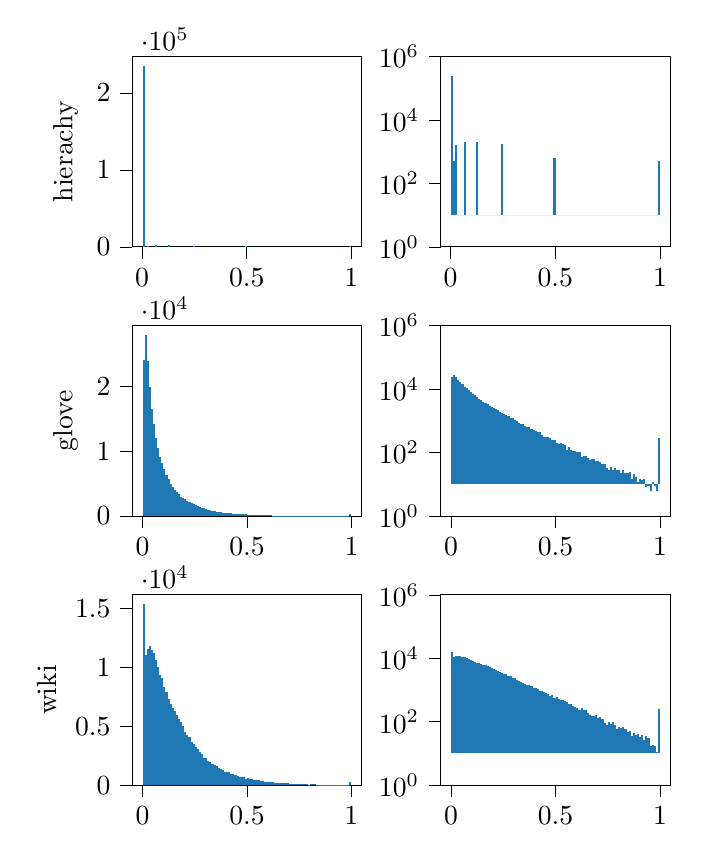
\begin{tikzpicture}

\definecolor{darkgray176}{RGB}{176,176,176}
\definecolor{steelblue31119180}{RGB}{31,119,180}

\begin{groupplot}[group style={group size=2 by 3}]
\nextgroupplot[
height=4cm,
tick align=outside,
tick pos=left,
width=4.5cm,
x grid style={darkgray176},
xmin=-0.04794921875, xmax=1.04990234375,
xtick style={color=black},
y grid style={darkgray176},
ylabel={hierachy},
ymin=0, ymax=247398.9,
ytick style={color=black}
]
\draw[draw=none,fill=steelblue31119180] (axis cs:0.001953125,0) rectangle (axis cs:0.01193359375,235618);
\draw[draw=none,fill=steelblue31119180] (axis cs:0.01193359375,0) rectangle (axis cs:0.0219140625,492);
\draw[draw=none,fill=steelblue31119180] (axis cs:0.0219140625,0) rectangle (axis cs:0.03189453125,1573);
\draw[draw=none,fill=steelblue31119180] (axis cs:0.03189453125,0) rectangle (axis cs:0.041875,0);
\draw[draw=none,fill=steelblue31119180] (axis cs:0.041875,0) rectangle (axis cs:0.05185546875,0);
\draw[draw=none,fill=steelblue31119180] (axis cs:0.05185546875,0) rectangle (axis cs:0.0618359375,0);
\draw[draw=none,fill=steelblue31119180] (axis cs:0.0618359375,0) rectangle (axis cs:0.07181640625,2022);
\draw[draw=none,fill=steelblue31119180] (axis cs:0.07181640625,0) rectangle (axis cs:0.081796875,0);
\draw[draw=none,fill=steelblue31119180] (axis cs:0.081796875,0) rectangle (axis cs:0.09177734375,0);
\draw[draw=none,fill=steelblue31119180] (axis cs:0.09177734375,0) rectangle (axis cs:0.1017578125,0);
\draw[draw=none,fill=steelblue31119180] (axis cs:0.1017578125,0) rectangle (axis cs:0.11173828125,0);
\draw[draw=none,fill=steelblue31119180] (axis cs:0.11173828125,0) rectangle (axis cs:0.12171875,0);
\draw[draw=none,fill=steelblue31119180] (axis cs:0.12171875,0) rectangle (axis cs:0.13169921875,1991);
\draw[draw=none,fill=steelblue31119180] (axis cs:0.13169921875,0) rectangle (axis cs:0.1416796875,0);
\draw[draw=none,fill=steelblue31119180] (axis cs:0.1416796875,0) rectangle (axis cs:0.15166015625,0);
\draw[draw=none,fill=steelblue31119180] (axis cs:0.15166015625,0) rectangle (axis cs:0.161640625,0);
\draw[draw=none,fill=steelblue31119180] (axis cs:0.161640625,0) rectangle (axis cs:0.17162109375,0);
\draw[draw=none,fill=steelblue31119180] (axis cs:0.17162109375,0) rectangle (axis cs:0.1816015625,0);
\draw[draw=none,fill=steelblue31119180] (axis cs:0.1816015625,0) rectangle (axis cs:0.19158203125,0);
\draw[draw=none,fill=steelblue31119180] (axis cs:0.19158203125,0) rectangle (axis cs:0.2015625,0);
\draw[draw=none,fill=steelblue31119180] (axis cs:0.2015625,0) rectangle (axis cs:0.21154296875,0);
\draw[draw=none,fill=steelblue31119180] (axis cs:0.21154296875,0) rectangle (axis cs:0.2215234375,0);
\draw[draw=none,fill=steelblue31119180] (axis cs:0.2215234375,0) rectangle (axis cs:0.23150390625,0);
\draw[draw=none,fill=steelblue31119180] (axis cs:0.23150390625,0) rectangle (axis cs:0.241484375,0);
\draw[draw=none,fill=steelblue31119180] (axis cs:0.241484375,0) rectangle (axis cs:0.25146484375,1780);
\draw[draw=none,fill=steelblue31119180] (axis cs:0.25146484375,0) rectangle (axis cs:0.2614453125,0);
\draw[draw=none,fill=steelblue31119180] (axis cs:0.2614453125,0) rectangle (axis cs:0.27142578125,0);
\draw[draw=none,fill=steelblue31119180] (axis cs:0.27142578125,0) rectangle (axis cs:0.28140625,0);
\draw[draw=none,fill=steelblue31119180] (axis cs:0.28140625,0) rectangle (axis cs:0.29138671875,0);
\draw[draw=none,fill=steelblue31119180] (axis cs:0.29138671875,0) rectangle (axis cs:0.3013671875,0);
\draw[draw=none,fill=steelblue31119180] (axis cs:0.3013671875,0) rectangle (axis cs:0.31134765625,0);
\draw[draw=none,fill=steelblue31119180] (axis cs:0.31134765625,0) rectangle (axis cs:0.321328125,0);
\draw[draw=none,fill=steelblue31119180] (axis cs:0.321328125,0) rectangle (axis cs:0.33130859375,0);
\draw[draw=none,fill=steelblue31119180] (axis cs:0.33130859375,0) rectangle (axis cs:0.3412890625,0);
\draw[draw=none,fill=steelblue31119180] (axis cs:0.3412890625,0) rectangle (axis cs:0.35126953125,0);
\draw[draw=none,fill=steelblue31119180] (axis cs:0.35126953125,0) rectangle (axis cs:0.36125,0);
\draw[draw=none,fill=steelblue31119180] (axis cs:0.36125,0) rectangle (axis cs:0.37123046875,0);
\draw[draw=none,fill=steelblue31119180] (axis cs:0.37123046875,0) rectangle (axis cs:0.3812109375,0);
\draw[draw=none,fill=steelblue31119180] (axis cs:0.3812109375,0) rectangle (axis cs:0.39119140625,0);
\draw[draw=none,fill=steelblue31119180] (axis cs:0.39119140625,0) rectangle (axis cs:0.401171875,0);
\draw[draw=none,fill=steelblue31119180] (axis cs:0.401171875,0) rectangle (axis cs:0.41115234375,0);
\draw[draw=none,fill=steelblue31119180] (axis cs:0.41115234375,0) rectangle (axis cs:0.4211328125,0);
\draw[draw=none,fill=steelblue31119180] (axis cs:0.4211328125,0) rectangle (axis cs:0.43111328125,0);
\draw[draw=none,fill=steelblue31119180] (axis cs:0.43111328125,0) rectangle (axis cs:0.44109375,0);
\draw[draw=none,fill=steelblue31119180] (axis cs:0.44109375,0) rectangle (axis cs:0.45107421875,0);
\draw[draw=none,fill=steelblue31119180] (axis cs:0.45107421875,0) rectangle (axis cs:0.4610546875,0);
\draw[draw=none,fill=steelblue31119180] (axis cs:0.4610546875,0) rectangle (axis cs:0.47103515625,0);
\draw[draw=none,fill=steelblue31119180] (axis cs:0.47103515625,0) rectangle (axis cs:0.481015625,0);
\draw[draw=none,fill=steelblue31119180] (axis cs:0.481015625,0) rectangle (axis cs:0.49099609375,0);
\draw[draw=none,fill=steelblue31119180] (axis cs:0.49099609375,0) rectangle (axis cs:0.5009765625,655);
\draw[draw=none,fill=steelblue31119180] (axis cs:0.5009765625,0) rectangle (axis cs:0.51095703125,0);
\draw[draw=none,fill=steelblue31119180] (axis cs:0.51095703125,0) rectangle (axis cs:0.5209375,0);
\draw[draw=none,fill=steelblue31119180] (axis cs:0.5209375,0) rectangle (axis cs:0.53091796875,0);
\draw[draw=none,fill=steelblue31119180] (axis cs:0.53091796875,0) rectangle (axis cs:0.5408984375,0);
\draw[draw=none,fill=steelblue31119180] (axis cs:0.5408984375,0) rectangle (axis cs:0.55087890625,0);
\draw[draw=none,fill=steelblue31119180] (axis cs:0.55087890625,0) rectangle (axis cs:0.560859375,0);
\draw[draw=none,fill=steelblue31119180] (axis cs:0.560859375,0) rectangle (axis cs:0.57083984375,0);
\draw[draw=none,fill=steelblue31119180] (axis cs:0.57083984375,0) rectangle (axis cs:0.5808203125,0);
\draw[draw=none,fill=steelblue31119180] (axis cs:0.5808203125,0) rectangle (axis cs:0.59080078125,0);
\draw[draw=none,fill=steelblue31119180] (axis cs:0.59080078125,0) rectangle (axis cs:0.60078125,0);
\draw[draw=none,fill=steelblue31119180] (axis cs:0.60078125,0) rectangle (axis cs:0.61076171875,0);
\draw[draw=none,fill=steelblue31119180] (axis cs:0.61076171875,0) rectangle (axis cs:0.6207421875,0);
\draw[draw=none,fill=steelblue31119180] (axis cs:0.6207421875,0) rectangle (axis cs:0.63072265625,0);
\draw[draw=none,fill=steelblue31119180] (axis cs:0.63072265625,0) rectangle (axis cs:0.640703125,0);
\draw[draw=none,fill=steelblue31119180] (axis cs:0.640703125,0) rectangle (axis cs:0.65068359375,0);
\draw[draw=none,fill=steelblue31119180] (axis cs:0.65068359375,0) rectangle (axis cs:0.6606640625,0);
\draw[draw=none,fill=steelblue31119180] (axis cs:0.6606640625,0) rectangle (axis cs:0.67064453125,0);
\draw[draw=none,fill=steelblue31119180] (axis cs:0.67064453125,0) rectangle (axis cs:0.680625,0);
\draw[draw=none,fill=steelblue31119180] (axis cs:0.680625,0) rectangle (axis cs:0.69060546875,0);
\draw[draw=none,fill=steelblue31119180] (axis cs:0.69060546875,0) rectangle (axis cs:0.7005859375,0);
\draw[draw=none,fill=steelblue31119180] (axis cs:0.7005859375,0) rectangle (axis cs:0.71056640625,0);
\draw[draw=none,fill=steelblue31119180] (axis cs:0.71056640625,0) rectangle (axis cs:0.720546875,0);
\draw[draw=none,fill=steelblue31119180] (axis cs:0.720546875,0) rectangle (axis cs:0.73052734375,0);
\draw[draw=none,fill=steelblue31119180] (axis cs:0.73052734375,0) rectangle (axis cs:0.7405078125,0);
\draw[draw=none,fill=steelblue31119180] (axis cs:0.7405078125,0) rectangle (axis cs:0.75048828125,0);
\draw[draw=none,fill=steelblue31119180] (axis cs:0.75048828125,0) rectangle (axis cs:0.76046875,0);
\draw[draw=none,fill=steelblue31119180] (axis cs:0.76046875,0) rectangle (axis cs:0.77044921875,0);
\draw[draw=none,fill=steelblue31119180] (axis cs:0.77044921875,0) rectangle (axis cs:0.7804296875,0);
\draw[draw=none,fill=steelblue31119180] (axis cs:0.7804296875,0) rectangle (axis cs:0.79041015625,0);
\draw[draw=none,fill=steelblue31119180] (axis cs:0.79041015625,0) rectangle (axis cs:0.800390625,0);
\draw[draw=none,fill=steelblue31119180] (axis cs:0.800390625,0) rectangle (axis cs:0.81037109375,0);
\draw[draw=none,fill=steelblue31119180] (axis cs:0.81037109375,0) rectangle (axis cs:0.8203515625,0);
\draw[draw=none,fill=steelblue31119180] (axis cs:0.8203515625,0) rectangle (axis cs:0.83033203125,0);
\draw[draw=none,fill=steelblue31119180] (axis cs:0.83033203125,0) rectangle (axis cs:0.8403125,0);
\draw[draw=none,fill=steelblue31119180] (axis cs:0.8403125,0) rectangle (axis cs:0.85029296875,0);
\draw[draw=none,fill=steelblue31119180] (axis cs:0.85029296875,0) rectangle (axis cs:0.8602734375,0);
\draw[draw=none,fill=steelblue31119180] (axis cs:0.8602734375,0) rectangle (axis cs:0.87025390625,0);
\draw[draw=none,fill=steelblue31119180] (axis cs:0.87025390625,0) rectangle (axis cs:0.880234375,0);
\draw[draw=none,fill=steelblue31119180] (axis cs:0.880234375,0) rectangle (axis cs:0.89021484375,0);
\draw[draw=none,fill=steelblue31119180] (axis cs:0.89021484375,0) rectangle (axis cs:0.9001953125,0);
\draw[draw=none,fill=steelblue31119180] (axis cs:0.9001953125,0) rectangle (axis cs:0.91017578125,0);
\draw[draw=none,fill=steelblue31119180] (axis cs:0.91017578125,0) rectangle (axis cs:0.92015625,0);
\draw[draw=none,fill=steelblue31119180] (axis cs:0.92015625,0) rectangle (axis cs:0.93013671875,0);
\draw[draw=none,fill=steelblue31119180] (axis cs:0.93013671875,0) rectangle (axis cs:0.9401171875,0);
\draw[draw=none,fill=steelblue31119180] (axis cs:0.9401171875,0) rectangle (axis cs:0.95009765625,0);
\draw[draw=none,fill=steelblue31119180] (axis cs:0.95009765625,0) rectangle (axis cs:0.960078125,0);
\draw[draw=none,fill=steelblue31119180] (axis cs:0.960078125,0) rectangle (axis cs:0.97005859375,0);
\draw[draw=none,fill=steelblue31119180] (axis cs:0.97005859375,0) rectangle (axis cs:0.9800390625,0);
\draw[draw=none,fill=steelblue31119180] (axis cs:0.9800390625,0) rectangle (axis cs:0.99001953125,0);
\draw[draw=none,fill=steelblue31119180] (axis cs:0.99001953125,0) rectangle (axis cs:1,519);

\nextgroupplot[
height=4cm,
log basis y={10},
tick align=outside,
tick pos=left,
width=4.5cm,
x grid style={darkgray176},
xmin=-0.04794921875, xmax=1.04990234375,
xtick style={color=black},
y grid style={darkgray176},
ymin=1, ymax=1000000,
ymode=log,
ytick style={color=black}
]
\draw[draw=none,fill=steelblue31119180] (axis cs:0.001953125,0) rectangle (axis cs:0.01193359375,235618);
\draw[draw=none,fill=steelblue31119180] (axis cs:0.01193359375,0) rectangle (axis cs:0.0219140625,492);
\draw[draw=none,fill=steelblue31119180] (axis cs:0.0219140625,0) rectangle (axis cs:0.03189453125,1573);
\draw[draw=none,fill=steelblue31119180] (axis cs:0.03189453125,0) rectangle (axis cs:0.041875,0);
\draw[draw=none,fill=steelblue31119180] (axis cs:0.041875,0) rectangle (axis cs:0.05185546875,0);
\draw[draw=none,fill=steelblue31119180] (axis cs:0.05185546875,0) rectangle (axis cs:0.0618359375,0);
\draw[draw=none,fill=steelblue31119180] (axis cs:0.0618359375,0) rectangle (axis cs:0.07181640625,2022);
\draw[draw=none,fill=steelblue31119180] (axis cs:0.07181640625,0) rectangle (axis cs:0.081796875,0);
\draw[draw=none,fill=steelblue31119180] (axis cs:0.081796875,0) rectangle (axis cs:0.09177734375,0);
\draw[draw=none,fill=steelblue31119180] (axis cs:0.09177734375,0) rectangle (axis cs:0.1017578125,0);
\draw[draw=none,fill=steelblue31119180] (axis cs:0.1017578125,0) rectangle (axis cs:0.11173828125,0);
\draw[draw=none,fill=steelblue31119180] (axis cs:0.11173828125,0) rectangle (axis cs:0.12171875,0);
\draw[draw=none,fill=steelblue31119180] (axis cs:0.12171875,0) rectangle (axis cs:0.13169921875,1991);
\draw[draw=none,fill=steelblue31119180] (axis cs:0.13169921875,0) rectangle (axis cs:0.1416796875,0);
\draw[draw=none,fill=steelblue31119180] (axis cs:0.1416796875,0) rectangle (axis cs:0.15166015625,0);
\draw[draw=none,fill=steelblue31119180] (axis cs:0.15166015625,0) rectangle (axis cs:0.161640625,0);
\draw[draw=none,fill=steelblue31119180] (axis cs:0.161640625,0) rectangle (axis cs:0.17162109375,0);
\draw[draw=none,fill=steelblue31119180] (axis cs:0.17162109375,0) rectangle (axis cs:0.1816015625,0);
\draw[draw=none,fill=steelblue31119180] (axis cs:0.1816015625,0) rectangle (axis cs:0.19158203125,0);
\draw[draw=none,fill=steelblue31119180] (axis cs:0.19158203125,0) rectangle (axis cs:0.2015625,0);
\draw[draw=none,fill=steelblue31119180] (axis cs:0.2015625,0) rectangle (axis cs:0.21154296875,0);
\draw[draw=none,fill=steelblue31119180] (axis cs:0.21154296875,0) rectangle (axis cs:0.2215234375,0);
\draw[draw=none,fill=steelblue31119180] (axis cs:0.2215234375,0) rectangle (axis cs:0.23150390625,0);
\draw[draw=none,fill=steelblue31119180] (axis cs:0.23150390625,0) rectangle (axis cs:0.241484375,0);
\draw[draw=none,fill=steelblue31119180] (axis cs:0.241484375,0) rectangle (axis cs:0.25146484375,1780);
\draw[draw=none,fill=steelblue31119180] (axis cs:0.25146484375,0) rectangle (axis cs:0.2614453125,0);
\draw[draw=none,fill=steelblue31119180] (axis cs:0.2614453125,0) rectangle (axis cs:0.27142578125,0);
\draw[draw=none,fill=steelblue31119180] (axis cs:0.27142578125,0) rectangle (axis cs:0.28140625,0);
\draw[draw=none,fill=steelblue31119180] (axis cs:0.28140625,0) rectangle (axis cs:0.29138671875,0);
\draw[draw=none,fill=steelblue31119180] (axis cs:0.29138671875,0) rectangle (axis cs:0.3013671875,0);
\draw[draw=none,fill=steelblue31119180] (axis cs:0.3013671875,0) rectangle (axis cs:0.31134765625,0);
\draw[draw=none,fill=steelblue31119180] (axis cs:0.31134765625,0) rectangle (axis cs:0.321328125,0);
\draw[draw=none,fill=steelblue31119180] (axis cs:0.321328125,0) rectangle (axis cs:0.33130859375,0);
\draw[draw=none,fill=steelblue31119180] (axis cs:0.33130859375,0) rectangle (axis cs:0.3412890625,0);
\draw[draw=none,fill=steelblue31119180] (axis cs:0.3412890625,0) rectangle (axis cs:0.35126953125,0);
\draw[draw=none,fill=steelblue31119180] (axis cs:0.35126953125,0) rectangle (axis cs:0.36125,0);
\draw[draw=none,fill=steelblue31119180] (axis cs:0.36125,0) rectangle (axis cs:0.37123046875,0);
\draw[draw=none,fill=steelblue31119180] (axis cs:0.37123046875,0) rectangle (axis cs:0.3812109375,0);
\draw[draw=none,fill=steelblue31119180] (axis cs:0.3812109375,0) rectangle (axis cs:0.39119140625,0);
\draw[draw=none,fill=steelblue31119180] (axis cs:0.39119140625,0) rectangle (axis cs:0.401171875,0);
\draw[draw=none,fill=steelblue31119180] (axis cs:0.401171875,0) rectangle (axis cs:0.41115234375,0);
\draw[draw=none,fill=steelblue31119180] (axis cs:0.41115234375,0) rectangle (axis cs:0.4211328125,0);
\draw[draw=none,fill=steelblue31119180] (axis cs:0.4211328125,0) rectangle (axis cs:0.43111328125,0);
\draw[draw=none,fill=steelblue31119180] (axis cs:0.43111328125,0) rectangle (axis cs:0.44109375,0);
\draw[draw=none,fill=steelblue31119180] (axis cs:0.44109375,0) rectangle (axis cs:0.45107421875,0);
\draw[draw=none,fill=steelblue31119180] (axis cs:0.45107421875,0) rectangle (axis cs:0.4610546875,0);
\draw[draw=none,fill=steelblue31119180] (axis cs:0.4610546875,0) rectangle (axis cs:0.47103515625,0);
\draw[draw=none,fill=steelblue31119180] (axis cs:0.47103515625,0) rectangle (axis cs:0.481015625,0);
\draw[draw=none,fill=steelblue31119180] (axis cs:0.481015625,0) rectangle (axis cs:0.49099609375,0);
\draw[draw=none,fill=steelblue31119180] (axis cs:0.49099609375,0) rectangle (axis cs:0.5009765625,655);
\draw[draw=none,fill=steelblue31119180] (axis cs:0.5009765625,0) rectangle (axis cs:0.51095703125,0);
\draw[draw=none,fill=steelblue31119180] (axis cs:0.51095703125,0) rectangle (axis cs:0.5209375,0);
\draw[draw=none,fill=steelblue31119180] (axis cs:0.5209375,0) rectangle (axis cs:0.53091796875,0);
\draw[draw=none,fill=steelblue31119180] (axis cs:0.53091796875,0) rectangle (axis cs:0.5408984375,0);
\draw[draw=none,fill=steelblue31119180] (axis cs:0.5408984375,0) rectangle (axis cs:0.55087890625,0);
\draw[draw=none,fill=steelblue31119180] (axis cs:0.55087890625,0) rectangle (axis cs:0.560859375,0);
\draw[draw=none,fill=steelblue31119180] (axis cs:0.560859375,0) rectangle (axis cs:0.57083984375,0);
\draw[draw=none,fill=steelblue31119180] (axis cs:0.57083984375,0) rectangle (axis cs:0.5808203125,0);
\draw[draw=none,fill=steelblue31119180] (axis cs:0.5808203125,0) rectangle (axis cs:0.59080078125,0);
\draw[draw=none,fill=steelblue31119180] (axis cs:0.59080078125,0) rectangle (axis cs:0.60078125,0);
\draw[draw=none,fill=steelblue31119180] (axis cs:0.60078125,0) rectangle (axis cs:0.61076171875,0);
\draw[draw=none,fill=steelblue31119180] (axis cs:0.61076171875,0) rectangle (axis cs:0.6207421875,0);
\draw[draw=none,fill=steelblue31119180] (axis cs:0.6207421875,0) rectangle (axis cs:0.63072265625,0);
\draw[draw=none,fill=steelblue31119180] (axis cs:0.63072265625,0) rectangle (axis cs:0.640703125,0);
\draw[draw=none,fill=steelblue31119180] (axis cs:0.640703125,0) rectangle (axis cs:0.65068359375,0);
\draw[draw=none,fill=steelblue31119180] (axis cs:0.65068359375,0) rectangle (axis cs:0.6606640625,0);
\draw[draw=none,fill=steelblue31119180] (axis cs:0.6606640625,0) rectangle (axis cs:0.67064453125,0);
\draw[draw=none,fill=steelblue31119180] (axis cs:0.67064453125,0) rectangle (axis cs:0.680625,0);
\draw[draw=none,fill=steelblue31119180] (axis cs:0.680625,0) rectangle (axis cs:0.69060546875,0);
\draw[draw=none,fill=steelblue31119180] (axis cs:0.69060546875,0) rectangle (axis cs:0.7005859375,0);
\draw[draw=none,fill=steelblue31119180] (axis cs:0.7005859375,0) rectangle (axis cs:0.71056640625,0);
\draw[draw=none,fill=steelblue31119180] (axis cs:0.71056640625,0) rectangle (axis cs:0.720546875,0);
\draw[draw=none,fill=steelblue31119180] (axis cs:0.720546875,0) rectangle (axis cs:0.73052734375,0);
\draw[draw=none,fill=steelblue31119180] (axis cs:0.73052734375,0) rectangle (axis cs:0.7405078125,0);
\draw[draw=none,fill=steelblue31119180] (axis cs:0.7405078125,0) rectangle (axis cs:0.75048828125,0);
\draw[draw=none,fill=steelblue31119180] (axis cs:0.75048828125,0) rectangle (axis cs:0.76046875,0);
\draw[draw=none,fill=steelblue31119180] (axis cs:0.76046875,0) rectangle (axis cs:0.77044921875,0);
\draw[draw=none,fill=steelblue31119180] (axis cs:0.77044921875,0) rectangle (axis cs:0.7804296875,0);
\draw[draw=none,fill=steelblue31119180] (axis cs:0.7804296875,0) rectangle (axis cs:0.79041015625,0);
\draw[draw=none,fill=steelblue31119180] (axis cs:0.79041015625,0) rectangle (axis cs:0.800390625,0);
\draw[draw=none,fill=steelblue31119180] (axis cs:0.800390625,0) rectangle (axis cs:0.81037109375,0);
\draw[draw=none,fill=steelblue31119180] (axis cs:0.81037109375,0) rectangle (axis cs:0.8203515625,0);
\draw[draw=none,fill=steelblue31119180] (axis cs:0.8203515625,0) rectangle (axis cs:0.83033203125,0);
\draw[draw=none,fill=steelblue31119180] (axis cs:0.83033203125,0) rectangle (axis cs:0.8403125,0);
\draw[draw=none,fill=steelblue31119180] (axis cs:0.8403125,0) rectangle (axis cs:0.85029296875,0);
\draw[draw=none,fill=steelblue31119180] (axis cs:0.85029296875,0) rectangle (axis cs:0.8602734375,0);
\draw[draw=none,fill=steelblue31119180] (axis cs:0.8602734375,0) rectangle (axis cs:0.87025390625,0);
\draw[draw=none,fill=steelblue31119180] (axis cs:0.87025390625,0) rectangle (axis cs:0.880234375,0);
\draw[draw=none,fill=steelblue31119180] (axis cs:0.880234375,0) rectangle (axis cs:0.89021484375,0);
\draw[draw=none,fill=steelblue31119180] (axis cs:0.89021484375,0) rectangle (axis cs:0.9001953125,0);
\draw[draw=none,fill=steelblue31119180] (axis cs:0.9001953125,0) rectangle (axis cs:0.91017578125,0);
\draw[draw=none,fill=steelblue31119180] (axis cs:0.91017578125,0) rectangle (axis cs:0.92015625,0);
\draw[draw=none,fill=steelblue31119180] (axis cs:0.92015625,0) rectangle (axis cs:0.93013671875,0);
\draw[draw=none,fill=steelblue31119180] (axis cs:0.93013671875,0) rectangle (axis cs:0.9401171875,0);
\draw[draw=none,fill=steelblue31119180] (axis cs:0.9401171875,0) rectangle (axis cs:0.95009765625,0);
\draw[draw=none,fill=steelblue31119180] (axis cs:0.95009765625,0) rectangle (axis cs:0.960078125,0);
\draw[draw=none,fill=steelblue31119180] (axis cs:0.960078125,0) rectangle (axis cs:0.97005859375,0);
\draw[draw=none,fill=steelblue31119180] (axis cs:0.97005859375,0) rectangle (axis cs:0.9800390625,0);
\draw[draw=none,fill=steelblue31119180] (axis cs:0.9800390625,0) rectangle (axis cs:0.99001953125,0);
\draw[draw=none,fill=steelblue31119180] (axis cs:0.99001953125,0) rectangle (axis cs:1,519);

\nextgroupplot[
height=4cm,
tick align=outside,
tick pos=left,
width=4.5cm,
x grid style={darkgray176},
xmin=-0.0499687628247378, xmax=1.04999851251546,
xtick style={color=black},
y grid style={darkgray176},
ylabel={glove},
ymin=0, ymax=29373.75,
ytick style={color=black}
]
\draw[draw=none,fill=steelblue31119180] (axis cs:2.97496907259529e-05,0) rectangle (axis cs:0.0100294521938187,24096);
\draw[draw=none,fill=steelblue31119180] (axis cs:0.0100294521938187,0) rectangle (axis cs:0.0200291546969114,27975);
\draw[draw=none,fill=steelblue31119180] (axis cs:0.0200291546969114,0) rectangle (axis cs:0.0300288572000042,23889);
\draw[draw=none,fill=steelblue31119180] (axis cs:0.0300288572000042,0) rectangle (axis cs:0.0400285597030969,19908);
\draw[draw=none,fill=steelblue31119180] (axis cs:0.0400285597030969,0) rectangle (axis cs:0.0500282622061897,16565);
\draw[draw=none,fill=steelblue31119180] (axis cs:0.0500282622061897,0) rectangle (axis cs:0.0600279647092824,14271);
\draw[draw=none,fill=steelblue31119180] (axis cs:0.0600279647092824,0) rectangle (axis cs:0.0700276672123751,12060);
\draw[draw=none,fill=steelblue31119180] (axis cs:0.0700276672123751,0) rectangle (axis cs:0.0800273697154679,10479);
\draw[draw=none,fill=steelblue31119180] (axis cs:0.0800273697154679,0) rectangle (axis cs:0.0900270722185606,9128);
\draw[draw=none,fill=steelblue31119180] (axis cs:0.0900270722185606,0) rectangle (axis cs:0.100026774721653,8199);
\draw[draw=none,fill=steelblue31119180] (axis cs:0.100026774721653,0) rectangle (axis cs:0.110026477224746,7228);
\draw[draw=none,fill=steelblue31119180] (axis cs:0.110026477224746,0) rectangle (axis cs:0.120026179727839,6410);
\draw[draw=none,fill=steelblue31119180] (axis cs:0.120026179727839,0) rectangle (axis cs:0.130025882230932,5654);
\draw[draw=none,fill=steelblue31119180] (axis cs:0.130025882230932,0) rectangle (axis cs:0.140025584734024,5004);
\draw[draw=none,fill=steelblue31119180] (axis cs:0.140025584734024,0) rectangle (axis cs:0.150025287237117,4529);
\draw[draw=none,fill=steelblue31119180] (axis cs:0.150025287237117,0) rectangle (axis cs:0.16002498974021,4043);
\draw[draw=none,fill=steelblue31119180] (axis cs:0.16002498974021,0) rectangle (axis cs:0.170024692243303,3732);
\draw[draw=none,fill=steelblue31119180] (axis cs:0.170024692243303,0) rectangle (axis cs:0.180024394746395,3412);
\draw[draw=none,fill=steelblue31119180] (axis cs:0.180024394746395,0) rectangle (axis cs:0.190024097249488,3009);
\draw[draw=none,fill=steelblue31119180] (axis cs:0.190024097249488,0) rectangle (axis cs:0.200023799752581,2830);
\draw[draw=none,fill=steelblue31119180] (axis cs:0.200023799752581,0) rectangle (axis cs:0.210023502255673,2556);
\draw[draw=none,fill=steelblue31119180] (axis cs:0.210023502255673,0) rectangle (axis cs:0.220023204758766,2288);
\draw[draw=none,fill=steelblue31119180] (axis cs:0.220023204758766,0) rectangle (axis cs:0.230022907261859,2183);
\draw[draw=none,fill=steelblue31119180] (axis cs:0.230022907261859,0) rectangle (axis cs:0.240022609764952,1950);
\draw[draw=none,fill=steelblue31119180] (axis cs:0.240022609764952,0) rectangle (axis cs:0.250022312268044,1813);
\draw[draw=none,fill=steelblue31119180] (axis cs:0.250022312268044,0) rectangle (axis cs:0.260022014771137,1693);
\draw[draw=none,fill=steelblue31119180] (axis cs:0.260022014771137,0) rectangle (axis cs:0.27002171727423,1554);
\draw[draw=none,fill=steelblue31119180] (axis cs:0.27002171727423,0) rectangle (axis cs:0.280021419777323,1390);
\draw[draw=none,fill=steelblue31119180] (axis cs:0.280021419777323,0) rectangle (axis cs:0.290021122280415,1268);
\draw[draw=none,fill=steelblue31119180] (axis cs:0.290021122280415,0) rectangle (axis cs:0.300020824783508,1218);
\draw[draw=none,fill=steelblue31119180] (axis cs:0.300020824783508,0) rectangle (axis cs:0.310020527286601,1090);
\draw[draw=none,fill=steelblue31119180] (axis cs:0.310020527286601,0) rectangle (axis cs:0.320020229789694,993);
\draw[draw=none,fill=steelblue31119180] (axis cs:0.320020229789694,0) rectangle (axis cs:0.330019932292786,873);
\draw[draw=none,fill=steelblue31119180] (axis cs:0.330019932292786,0) rectangle (axis cs:0.340019634795879,817);
\draw[draw=none,fill=steelblue31119180] (axis cs:0.340019634795879,0) rectangle (axis cs:0.350019337298972,792);
\draw[draw=none,fill=steelblue31119180] (axis cs:0.350019337298972,0) rectangle (axis cs:0.360019039802065,687);
\draw[draw=none,fill=steelblue31119180] (axis cs:0.360019039802065,0) rectangle (axis cs:0.370018742305157,636);
\draw[draw=none,fill=steelblue31119180] (axis cs:0.370018742305157,0) rectangle (axis cs:0.38001844480825,640);
\draw[draw=none,fill=steelblue31119180] (axis cs:0.38001844480825,0) rectangle (axis cs:0.390018147311343,534);
\draw[draw=none,fill=steelblue31119180] (axis cs:0.390018147311343,0) rectangle (axis cs:0.400017849814436,524);
\draw[draw=none,fill=steelblue31119180] (axis cs:0.400017849814436,0) rectangle (axis cs:0.410017552317528,494);
\draw[draw=none,fill=steelblue31119180] (axis cs:0.410017552317528,0) rectangle (axis cs:0.420017254820621,431);
\draw[draw=none,fill=steelblue31119180] (axis cs:0.420017254820621,0) rectangle (axis cs:0.430016957323714,440);
\draw[draw=none,fill=steelblue31119180] (axis cs:0.430016957323714,0) rectangle (axis cs:0.440016659826807,371);
\draw[draw=none,fill=steelblue31119180] (axis cs:0.440016659826807,0) rectangle (axis cs:0.450016362329899,307);
\draw[draw=none,fill=steelblue31119180] (axis cs:0.450016362329899,0) rectangle (axis cs:0.460016064832992,307);
\draw[draw=none,fill=steelblue31119180] (axis cs:0.460016064832992,0) rectangle (axis cs:0.470015767336085,314);
\draw[draw=none,fill=steelblue31119180] (axis cs:0.470015767336085,0) rectangle (axis cs:0.480015469839177,292);
\draw[draw=none,fill=steelblue31119180] (axis cs:0.480015469839178,0) rectangle (axis cs:0.49001517234227,241);
\draw[draw=none,fill=steelblue31119180] (axis cs:0.49001517234227,0) rectangle (axis cs:0.500014874845363,250);
\draw[draw=none,fill=steelblue31119180] (axis cs:0.500014874845363,0) rectangle (axis cs:0.510014577348456,206);
\draw[draw=none,fill=steelblue31119180] (axis cs:0.510014577348456,0) rectangle (axis cs:0.520014279851548,185);
\draw[draw=none,fill=steelblue31119180] (axis cs:0.520014279851549,0) rectangle (axis cs:0.530013982354641,204);
\draw[draw=none,fill=steelblue31119180] (axis cs:0.530013982354641,0) rectangle (axis cs:0.540013684857734,191);
\draw[draw=none,fill=steelblue31119180] (axis cs:0.540013684857734,0) rectangle (axis cs:0.550013387360827,171);
\draw[draw=none,fill=steelblue31119180] (axis cs:0.550013387360827,0) rectangle (axis cs:0.56001308986392,125);
\draw[draw=none,fill=steelblue31119180] (axis cs:0.56001308986392,0) rectangle (axis cs:0.570012792367012,149);
\draw[draw=none,fill=steelblue31119180] (axis cs:0.570012792367012,0) rectangle (axis cs:0.580012494870105,123);
\draw[draw=none,fill=steelblue31119180] (axis cs:0.580012494870105,0) rectangle (axis cs:0.590012197373198,109);
\draw[draw=none,fill=steelblue31119180] (axis cs:0.590012197373198,0) rectangle (axis cs:0.600011899876291,114);
\draw[draw=none,fill=steelblue31119180] (axis cs:0.60001189987629,0) rectangle (axis cs:0.610011602379383,101);
\draw[draw=none,fill=steelblue31119180] (axis cs:0.610011602379383,0) rectangle (axis cs:0.620011304882476,102);
\draw[draw=none,fill=steelblue31119180] (axis cs:0.620011304882476,0) rectangle (axis cs:0.630011007385569,74);
\draw[draw=none,fill=steelblue31119180] (axis cs:0.630011007385569,0) rectangle (axis cs:0.640010709888661,78);
\draw[draw=none,fill=steelblue31119180] (axis cs:0.640010709888661,0) rectangle (axis cs:0.650010412391754,79);
\draw[draw=none,fill=steelblue31119180] (axis cs:0.650010412391754,0) rectangle (axis cs:0.660010114894847,69);
\draw[draw=none,fill=steelblue31119180] (axis cs:0.660010114894847,0) rectangle (axis cs:0.67000981739794,58);
\draw[draw=none,fill=steelblue31119180] (axis cs:0.67000981739794,0) rectangle (axis cs:0.680009519901032,61);
\draw[draw=none,fill=steelblue31119180] (axis cs:0.680009519901032,0) rectangle (axis cs:0.690009222404125,64);
\draw[draw=none,fill=steelblue31119180] (axis cs:0.690009222404125,0) rectangle (axis cs:0.700008924907218,54);
\draw[draw=none,fill=steelblue31119180] (axis cs:0.700008924907218,0) rectangle (axis cs:0.710008627410311,53);
\draw[draw=none,fill=steelblue31119180] (axis cs:0.710008627410311,0) rectangle (axis cs:0.720008329913403,50);
\draw[draw=none,fill=steelblue31119180] (axis cs:0.720008329913403,0) rectangle (axis cs:0.730008032416496,43);
\draw[draw=none,fill=steelblue31119180] (axis cs:0.730008032416496,0) rectangle (axis cs:0.740007734919589,45);
\draw[draw=none,fill=steelblue31119180] (axis cs:0.740007734919589,0) rectangle (axis cs:0.750007437422681,33);
\draw[draw=none,fill=steelblue31119180] (axis cs:0.750007437422681,0) rectangle (axis cs:0.760007139925774,29);
\draw[draw=none,fill=steelblue31119180] (axis cs:0.760007139925774,0) rectangle (axis cs:0.770006842428867,36);
\draw[draw=none,fill=steelblue31119180] (axis cs:0.770006842428867,0) rectangle (axis cs:0.78000654493196,28);
\draw[draw=none,fill=steelblue31119180] (axis cs:0.78000654493196,0) rectangle (axis cs:0.790006247435052,33);
\draw[draw=none,fill=steelblue31119180] (axis cs:0.790006247435052,0) rectangle (axis cs:0.800005949938145,29);
\draw[draw=none,fill=steelblue31119180] (axis cs:0.800005949938145,0) rectangle (axis cs:0.810005652441238,28);
\draw[draw=none,fill=steelblue31119180] (axis cs:0.810005652441238,0) rectangle (axis cs:0.820005354944331,22);
\draw[draw=none,fill=steelblue31119180] (axis cs:0.820005354944331,0) rectangle (axis cs:0.830005057447423,28);
\draw[draw=none,fill=steelblue31119180] (axis cs:0.830005057447423,0) rectangle (axis cs:0.840004759950516,22);
\draw[draw=none,fill=steelblue31119180] (axis cs:0.840004759950516,0) rectangle (axis cs:0.850004462453609,23);
\draw[draw=none,fill=steelblue31119180] (axis cs:0.850004462453609,0) rectangle (axis cs:0.860004164956702,25);
\draw[draw=none,fill=steelblue31119180] (axis cs:0.860004164956702,0) rectangle (axis cs:0.870003867459794,15);
\draw[draw=none,fill=steelblue31119180] (axis cs:0.870003867459795,0) rectangle (axis cs:0.880003569962887,21);
\draw[draw=none,fill=steelblue31119180] (axis cs:0.880003569962887,0) rectangle (axis cs:0.89000327246598,17);
\draw[draw=none,fill=steelblue31119180] (axis cs:0.89000327246598,0) rectangle (axis cs:0.900002974969073,12);
\draw[draw=none,fill=steelblue31119180] (axis cs:0.900002974969073,0) rectangle (axis cs:0.910002677472165,15);
\draw[draw=none,fill=steelblue31119180] (axis cs:0.910002677472165,0) rectangle (axis cs:0.920002379975258,14);
\draw[draw=none,fill=steelblue31119180] (axis cs:0.920002379975258,0) rectangle (axis cs:0.930002082478351,15);
\draw[draw=none,fill=steelblue31119180] (axis cs:0.930002082478351,0) rectangle (axis cs:0.940001784981444,8);
\draw[draw=none,fill=steelblue31119180] (axis cs:0.940001784981444,0) rectangle (axis cs:0.950001487484536,9);
\draw[draw=none,fill=steelblue31119180] (axis cs:0.950001487484536,0) rectangle (axis cs:0.960001189987629,6);
\draw[draw=none,fill=steelblue31119180] (axis cs:0.960001189987629,0) rectangle (axis cs:0.970000892490722,12);
\draw[draw=none,fill=steelblue31119180] (axis cs:0.970000892490722,0) rectangle (axis cs:0.980000594993815,9);
\draw[draw=none,fill=steelblue31119180] (axis cs:0.980000594993815,0) rectangle (axis cs:0.990000297496907,6);
\draw[draw=none,fill=steelblue31119180] (axis cs:0.990000297496907,0) rectangle (axis cs:1,280);

\nextgroupplot[
height=4cm,
log basis y={10},
tick align=outside,
tick pos=left,
width=4.5cm,
x grid style={darkgray176},
xmin=-0.0499687628247378, xmax=1.04999851251546,
xtick style={color=black},
y grid style={darkgray176},
ymin=1, ymax=1000000,
ymode=log,
ytick style={color=black}
]
\draw[draw=none,fill=steelblue31119180] (axis cs:2.97496907259529e-05,0) rectangle (axis cs:0.0100294521938187,24096);
\draw[draw=none,fill=steelblue31119180] (axis cs:0.0100294521938187,0) rectangle (axis cs:0.0200291546969114,27975);
\draw[draw=none,fill=steelblue31119180] (axis cs:0.0200291546969114,0) rectangle (axis cs:0.0300288572000042,23889);
\draw[draw=none,fill=steelblue31119180] (axis cs:0.0300288572000042,0) rectangle (axis cs:0.0400285597030969,19908);
\draw[draw=none,fill=steelblue31119180] (axis cs:0.0400285597030969,0) rectangle (axis cs:0.0500282622061897,16565);
\draw[draw=none,fill=steelblue31119180] (axis cs:0.0500282622061897,0) rectangle (axis cs:0.0600279647092824,14271);
\draw[draw=none,fill=steelblue31119180] (axis cs:0.0600279647092824,0) rectangle (axis cs:0.0700276672123751,12060);
\draw[draw=none,fill=steelblue31119180] (axis cs:0.0700276672123751,0) rectangle (axis cs:0.0800273697154679,10479);
\draw[draw=none,fill=steelblue31119180] (axis cs:0.0800273697154679,0) rectangle (axis cs:0.0900270722185606,9128);
\draw[draw=none,fill=steelblue31119180] (axis cs:0.0900270722185606,0) rectangle (axis cs:0.100026774721653,8199);
\draw[draw=none,fill=steelblue31119180] (axis cs:0.100026774721653,0) rectangle (axis cs:0.110026477224746,7228);
\draw[draw=none,fill=steelblue31119180] (axis cs:0.110026477224746,0) rectangle (axis cs:0.120026179727839,6410);
\draw[draw=none,fill=steelblue31119180] (axis cs:0.120026179727839,0) rectangle (axis cs:0.130025882230932,5654);
\draw[draw=none,fill=steelblue31119180] (axis cs:0.130025882230932,0) rectangle (axis cs:0.140025584734024,5004);
\draw[draw=none,fill=steelblue31119180] (axis cs:0.140025584734024,0) rectangle (axis cs:0.150025287237117,4529);
\draw[draw=none,fill=steelblue31119180] (axis cs:0.150025287237117,0) rectangle (axis cs:0.16002498974021,4043);
\draw[draw=none,fill=steelblue31119180] (axis cs:0.16002498974021,0) rectangle (axis cs:0.170024692243303,3732);
\draw[draw=none,fill=steelblue31119180] (axis cs:0.170024692243303,0) rectangle (axis cs:0.180024394746395,3412);
\draw[draw=none,fill=steelblue31119180] (axis cs:0.180024394746395,0) rectangle (axis cs:0.190024097249488,3009);
\draw[draw=none,fill=steelblue31119180] (axis cs:0.190024097249488,0) rectangle (axis cs:0.200023799752581,2830);
\draw[draw=none,fill=steelblue31119180] (axis cs:0.200023799752581,0) rectangle (axis cs:0.210023502255673,2556);
\draw[draw=none,fill=steelblue31119180] (axis cs:0.210023502255673,0) rectangle (axis cs:0.220023204758766,2288);
\draw[draw=none,fill=steelblue31119180] (axis cs:0.220023204758766,0) rectangle (axis cs:0.230022907261859,2183);
\draw[draw=none,fill=steelblue31119180] (axis cs:0.230022907261859,0) rectangle (axis cs:0.240022609764952,1950);
\draw[draw=none,fill=steelblue31119180] (axis cs:0.240022609764952,0) rectangle (axis cs:0.250022312268044,1813);
\draw[draw=none,fill=steelblue31119180] (axis cs:0.250022312268044,0) rectangle (axis cs:0.260022014771137,1693);
\draw[draw=none,fill=steelblue31119180] (axis cs:0.260022014771137,0) rectangle (axis cs:0.27002171727423,1554);
\draw[draw=none,fill=steelblue31119180] (axis cs:0.27002171727423,0) rectangle (axis cs:0.280021419777323,1390);
\draw[draw=none,fill=steelblue31119180] (axis cs:0.280021419777323,0) rectangle (axis cs:0.290021122280415,1268);
\draw[draw=none,fill=steelblue31119180] (axis cs:0.290021122280415,0) rectangle (axis cs:0.300020824783508,1218);
\draw[draw=none,fill=steelblue31119180] (axis cs:0.300020824783508,0) rectangle (axis cs:0.310020527286601,1090);
\draw[draw=none,fill=steelblue31119180] (axis cs:0.310020527286601,0) rectangle (axis cs:0.320020229789694,993);
\draw[draw=none,fill=steelblue31119180] (axis cs:0.320020229789694,0) rectangle (axis cs:0.330019932292786,873);
\draw[draw=none,fill=steelblue31119180] (axis cs:0.330019932292786,0) rectangle (axis cs:0.340019634795879,817);
\draw[draw=none,fill=steelblue31119180] (axis cs:0.340019634795879,0) rectangle (axis cs:0.350019337298972,792);
\draw[draw=none,fill=steelblue31119180] (axis cs:0.350019337298972,0) rectangle (axis cs:0.360019039802065,687);
\draw[draw=none,fill=steelblue31119180] (axis cs:0.360019039802065,0) rectangle (axis cs:0.370018742305157,636);
\draw[draw=none,fill=steelblue31119180] (axis cs:0.370018742305157,0) rectangle (axis cs:0.38001844480825,640);
\draw[draw=none,fill=steelblue31119180] (axis cs:0.38001844480825,0) rectangle (axis cs:0.390018147311343,534);
\draw[draw=none,fill=steelblue31119180] (axis cs:0.390018147311343,0) rectangle (axis cs:0.400017849814436,524);
\draw[draw=none,fill=steelblue31119180] (axis cs:0.400017849814436,0) rectangle (axis cs:0.410017552317528,494);
\draw[draw=none,fill=steelblue31119180] (axis cs:0.410017552317528,0) rectangle (axis cs:0.420017254820621,431);
\draw[draw=none,fill=steelblue31119180] (axis cs:0.420017254820621,0) rectangle (axis cs:0.430016957323714,440);
\draw[draw=none,fill=steelblue31119180] (axis cs:0.430016957323714,0) rectangle (axis cs:0.440016659826807,371);
\draw[draw=none,fill=steelblue31119180] (axis cs:0.440016659826807,0) rectangle (axis cs:0.450016362329899,307);
\draw[draw=none,fill=steelblue31119180] (axis cs:0.450016362329899,0) rectangle (axis cs:0.460016064832992,307);
\draw[draw=none,fill=steelblue31119180] (axis cs:0.460016064832992,0) rectangle (axis cs:0.470015767336085,314);
\draw[draw=none,fill=steelblue31119180] (axis cs:0.470015767336085,0) rectangle (axis cs:0.480015469839177,292);
\draw[draw=none,fill=steelblue31119180] (axis cs:0.480015469839178,0) rectangle (axis cs:0.49001517234227,241);
\draw[draw=none,fill=steelblue31119180] (axis cs:0.49001517234227,0) rectangle (axis cs:0.500014874845363,250);
\draw[draw=none,fill=steelblue31119180] (axis cs:0.500014874845363,0) rectangle (axis cs:0.510014577348456,206);
\draw[draw=none,fill=steelblue31119180] (axis cs:0.510014577348456,0) rectangle (axis cs:0.520014279851548,185);
\draw[draw=none,fill=steelblue31119180] (axis cs:0.520014279851549,0) rectangle (axis cs:0.530013982354641,204);
\draw[draw=none,fill=steelblue31119180] (axis cs:0.530013982354641,0) rectangle (axis cs:0.540013684857734,191);
\draw[draw=none,fill=steelblue31119180] (axis cs:0.540013684857734,0) rectangle (axis cs:0.550013387360827,171);
\draw[draw=none,fill=steelblue31119180] (axis cs:0.550013387360827,0) rectangle (axis cs:0.56001308986392,125);
\draw[draw=none,fill=steelblue31119180] (axis cs:0.56001308986392,0) rectangle (axis cs:0.570012792367012,149);
\draw[draw=none,fill=steelblue31119180] (axis cs:0.570012792367012,0) rectangle (axis cs:0.580012494870105,123);
\draw[draw=none,fill=steelblue31119180] (axis cs:0.580012494870105,0) rectangle (axis cs:0.590012197373198,109);
\draw[draw=none,fill=steelblue31119180] (axis cs:0.590012197373198,0) rectangle (axis cs:0.600011899876291,114);
\draw[draw=none,fill=steelblue31119180] (axis cs:0.60001189987629,0) rectangle (axis cs:0.610011602379383,101);
\draw[draw=none,fill=steelblue31119180] (axis cs:0.610011602379383,0) rectangle (axis cs:0.620011304882476,102);
\draw[draw=none,fill=steelblue31119180] (axis cs:0.620011304882476,0) rectangle (axis cs:0.630011007385569,74);
\draw[draw=none,fill=steelblue31119180] (axis cs:0.630011007385569,0) rectangle (axis cs:0.640010709888661,78);
\draw[draw=none,fill=steelblue31119180] (axis cs:0.640010709888661,0) rectangle (axis cs:0.650010412391754,79);
\draw[draw=none,fill=steelblue31119180] (axis cs:0.650010412391754,0) rectangle (axis cs:0.660010114894847,69);
\draw[draw=none,fill=steelblue31119180] (axis cs:0.660010114894847,0) rectangle (axis cs:0.67000981739794,58);
\draw[draw=none,fill=steelblue31119180] (axis cs:0.67000981739794,0) rectangle (axis cs:0.680009519901032,61);
\draw[draw=none,fill=steelblue31119180] (axis cs:0.680009519901032,0) rectangle (axis cs:0.690009222404125,64);
\draw[draw=none,fill=steelblue31119180] (axis cs:0.690009222404125,0) rectangle (axis cs:0.700008924907218,54);
\draw[draw=none,fill=steelblue31119180] (axis cs:0.700008924907218,0) rectangle (axis cs:0.710008627410311,53);
\draw[draw=none,fill=steelblue31119180] (axis cs:0.710008627410311,0) rectangle (axis cs:0.720008329913403,50);
\draw[draw=none,fill=steelblue31119180] (axis cs:0.720008329913403,0) rectangle (axis cs:0.730008032416496,43);
\draw[draw=none,fill=steelblue31119180] (axis cs:0.730008032416496,0) rectangle (axis cs:0.740007734919589,45);
\draw[draw=none,fill=steelblue31119180] (axis cs:0.740007734919589,0) rectangle (axis cs:0.750007437422681,33);
\draw[draw=none,fill=steelblue31119180] (axis cs:0.750007437422681,0) rectangle (axis cs:0.760007139925774,29);
\draw[draw=none,fill=steelblue31119180] (axis cs:0.760007139925774,0) rectangle (axis cs:0.770006842428867,36);
\draw[draw=none,fill=steelblue31119180] (axis cs:0.770006842428867,0) rectangle (axis cs:0.78000654493196,28);
\draw[draw=none,fill=steelblue31119180] (axis cs:0.78000654493196,0) rectangle (axis cs:0.790006247435052,33);
\draw[draw=none,fill=steelblue31119180] (axis cs:0.790006247435052,0) rectangle (axis cs:0.800005949938145,29);
\draw[draw=none,fill=steelblue31119180] (axis cs:0.800005949938145,0) rectangle (axis cs:0.810005652441238,28);
\draw[draw=none,fill=steelblue31119180] (axis cs:0.810005652441238,0) rectangle (axis cs:0.820005354944331,22);
\draw[draw=none,fill=steelblue31119180] (axis cs:0.820005354944331,0) rectangle (axis cs:0.830005057447423,28);
\draw[draw=none,fill=steelblue31119180] (axis cs:0.830005057447423,0) rectangle (axis cs:0.840004759950516,22);
\draw[draw=none,fill=steelblue31119180] (axis cs:0.840004759950516,0) rectangle (axis cs:0.850004462453609,23);
\draw[draw=none,fill=steelblue31119180] (axis cs:0.850004462453609,0) rectangle (axis cs:0.860004164956702,25);
\draw[draw=none,fill=steelblue31119180] (axis cs:0.860004164956702,0) rectangle (axis cs:0.870003867459794,15);
\draw[draw=none,fill=steelblue31119180] (axis cs:0.870003867459795,0) rectangle (axis cs:0.880003569962887,21);
\draw[draw=none,fill=steelblue31119180] (axis cs:0.880003569962887,0) rectangle (axis cs:0.89000327246598,17);
\draw[draw=none,fill=steelblue31119180] (axis cs:0.89000327246598,0) rectangle (axis cs:0.900002974969073,12);
\draw[draw=none,fill=steelblue31119180] (axis cs:0.900002974969073,0) rectangle (axis cs:0.910002677472165,15);
\draw[draw=none,fill=steelblue31119180] (axis cs:0.910002677472165,0) rectangle (axis cs:0.920002379975258,14);
\draw[draw=none,fill=steelblue31119180] (axis cs:0.920002379975258,0) rectangle (axis cs:0.930002082478351,15);
\draw[draw=none,fill=steelblue31119180] (axis cs:0.930002082478351,0) rectangle (axis cs:0.940001784981444,8);
\draw[draw=none,fill=steelblue31119180] (axis cs:0.940001784981444,0) rectangle (axis cs:0.950001487484536,9);
\draw[draw=none,fill=steelblue31119180] (axis cs:0.950001487484536,0) rectangle (axis cs:0.960001189987629,6);
\draw[draw=none,fill=steelblue31119180] (axis cs:0.960001189987629,0) rectangle (axis cs:0.970000892490722,12);
\draw[draw=none,fill=steelblue31119180] (axis cs:0.970000892490722,0) rectangle (axis cs:0.980000594993815,9);
\draw[draw=none,fill=steelblue31119180] (axis cs:0.980000594993815,0) rectangle (axis cs:0.990000297496907,6);
\draw[draw=none,fill=steelblue31119180] (axis cs:0.990000297496907,0) rectangle (axis cs:1,280);

\nextgroupplot[
height=4cm,
tick align=outside,
tick pos=left,
width=4.5cm,
x grid style={darkgray176},
xmin=-0.0499935305753595, xmax=1.04999969193216,
xtick style={color=black},
y grid style={darkgray176},
ylabel={wiki},
ymin=0, ymax=16153.2,
ytick style={color=black}
]
\draw[draw=none,fill=steelblue31119180] (axis cs:6.16135680043487e-06,0) rectangle (axis cs:0.0100060997432324,15384);
\draw[draw=none,fill=steelblue31119180] (axis cs:0.0100060997432324,0) rectangle (axis cs:0.0200060381296644,11033);
\draw[draw=none,fill=steelblue31119180] (axis cs:0.0200060381296644,0) rectangle (axis cs:0.0300059765160964,11579);
\draw[draw=none,fill=steelblue31119180] (axis cs:0.0300059765160964,0) rectangle (axis cs:0.0400059149025284,11770);
\draw[draw=none,fill=steelblue31119180] (axis cs:0.0400059149025284,0) rectangle (axis cs:0.0500058532889604,11467);
\draw[draw=none,fill=steelblue31119180] (axis cs:0.0500058532889604,0) rectangle (axis cs:0.0600057916753924,11179);
\draw[draw=none,fill=steelblue31119180] (axis cs:0.0600057916753924,0) rectangle (axis cs:0.0700057300618244,10645);
\draw[draw=none,fill=steelblue31119180] (axis cs:0.0700057300618244,0) rectangle (axis cs:0.0800056684482564,10056);
\draw[draw=none,fill=steelblue31119180] (axis cs:0.0800056684482564,0) rectangle (axis cs:0.0900056068346884,9391);
\draw[draw=none,fill=steelblue31119180] (axis cs:0.0900056068346884,0) rectangle (axis cs:0.10000554522112,9087);
\draw[draw=none,fill=steelblue31119180] (axis cs:0.10000554522112,0) rectangle (axis cs:0.110005483607552,8365);
\draw[draw=none,fill=steelblue31119180] (axis cs:0.110005483607552,0) rectangle (axis cs:0.120005421993984,7893);
\draw[draw=none,fill=steelblue31119180] (axis cs:0.120005421993984,0) rectangle (axis cs:0.130005360380416,7332);
\draw[draw=none,fill=steelblue31119180] (axis cs:0.130005360380416,0) rectangle (axis cs:0.140005298766848,6921);
\draw[draw=none,fill=steelblue31119180] (axis cs:0.140005298766848,0) rectangle (axis cs:0.15000523715328,6578);
\draw[draw=none,fill=steelblue31119180] (axis cs:0.15000523715328,0) rectangle (axis cs:0.160005175539712,6293);
\draw[draw=none,fill=steelblue31119180] (axis cs:0.160005175539712,0) rectangle (axis cs:0.170005113926144,5975);
\draw[draw=none,fill=steelblue31119180] (axis cs:0.170005113926144,0) rectangle (axis cs:0.180005052312576,5579);
\draw[draw=none,fill=steelblue31119180] (axis cs:0.180005052312576,0) rectangle (axis cs:0.190004990699008,5335);
\draw[draw=none,fill=steelblue31119180] (axis cs:0.190004990699008,0) rectangle (axis cs:0.20000492908544,5038);
\draw[draw=none,fill=steelblue31119180] (axis cs:0.20000492908544,0) rectangle (axis cs:0.210004867471872,4542);
\draw[draw=none,fill=steelblue31119180] (axis cs:0.210004867471872,0) rectangle (axis cs:0.220004805858304,4248);
\draw[draw=none,fill=steelblue31119180] (axis cs:0.220004805858304,0) rectangle (axis cs:0.230004744244736,4067);
\draw[draw=none,fill=steelblue31119180] (axis cs:0.230004744244736,0) rectangle (axis cs:0.240004682631168,3643);
\draw[draw=none,fill=steelblue31119180] (axis cs:0.240004682631168,0) rectangle (axis cs:0.2500046210176,3493);
\draw[draw=none,fill=steelblue31119180] (axis cs:0.2500046210176,0) rectangle (axis cs:0.260004559404032,3205);
\draw[draw=none,fill=steelblue31119180] (axis cs:0.260004559404032,0) rectangle (axis cs:0.270004497790464,3108);
\draw[draw=none,fill=steelblue31119180] (axis cs:0.270004497790464,0) rectangle (axis cs:0.280004436176896,2831);
\draw[draw=none,fill=steelblue31119180] (axis cs:0.280004436176896,0) rectangle (axis cs:0.290004374563328,2689);
\draw[draw=none,fill=steelblue31119180] (axis cs:0.290004374563328,0) rectangle (axis cs:0.30000431294976,2331);
\draw[draw=none,fill=steelblue31119180] (axis cs:0.30000431294976,0) rectangle (axis cs:0.310004251336192,2343);
\draw[draw=none,fill=steelblue31119180] (axis cs:0.310004251336192,0) rectangle (axis cs:0.320004189722624,2082);
\draw[draw=none,fill=steelblue31119180] (axis cs:0.320004189722624,0) rectangle (axis cs:0.330004128109056,1986);
\draw[draw=none,fill=steelblue31119180] (axis cs:0.330004128109056,0) rectangle (axis cs:0.340004066495488,1803);
\draw[draw=none,fill=steelblue31119180] (axis cs:0.340004066495488,0) rectangle (axis cs:0.35000400488192,1674);
\draw[draw=none,fill=steelblue31119180] (axis cs:0.35000400488192,0) rectangle (axis cs:0.360003943268352,1594);
\draw[draw=none,fill=steelblue31119180] (axis cs:0.360003943268352,0) rectangle (axis cs:0.370003881654784,1485);
\draw[draw=none,fill=steelblue31119180] (axis cs:0.370003881654784,0) rectangle (axis cs:0.380003820041216,1404);
\draw[draw=none,fill=steelblue31119180] (axis cs:0.380003820041216,0) rectangle (axis cs:0.390003758427648,1312);
\draw[draw=none,fill=steelblue31119180] (axis cs:0.390003758427648,0) rectangle (axis cs:0.40000369681408,1161);
\draw[draw=none,fill=steelblue31119180] (axis cs:0.40000369681408,0) rectangle (axis cs:0.410003635200512,1157);
\draw[draw=none,fill=steelblue31119180] (axis cs:0.410003635200512,0) rectangle (axis cs:0.420003573586944,1083);
\draw[draw=none,fill=steelblue31119180] (axis cs:0.420003573586944,0) rectangle (axis cs:0.430003511973376,950);
\draw[draw=none,fill=steelblue31119180] (axis cs:0.430003511973376,0) rectangle (axis cs:0.440003450359808,920);
\draw[draw=none,fill=steelblue31119180] (axis cs:0.440003450359808,0) rectangle (axis cs:0.45000338874624,854);
\draw[draw=none,fill=steelblue31119180] (axis cs:0.45000338874624,0) rectangle (axis cs:0.460003327132672,802);
\draw[draw=none,fill=steelblue31119180] (axis cs:0.460003327132672,0) rectangle (axis cs:0.470003265519104,738);
\draw[draw=none,fill=steelblue31119180] (axis cs:0.470003265519104,0) rectangle (axis cs:0.480003203905536,671);
\draw[draw=none,fill=steelblue31119180] (axis cs:0.480003203905536,0) rectangle (axis cs:0.490003142291968,688);
\draw[draw=none,fill=steelblue31119180] (axis cs:0.490003142291968,0) rectangle (axis cs:0.5000030806784,567);
\draw[draw=none,fill=steelblue31119180] (axis cs:0.5000030806784,0) rectangle (axis cs:0.510003019064832,601);
\draw[draw=none,fill=steelblue31119180] (axis cs:0.510003019064832,0) rectangle (axis cs:0.520002957451264,517);
\draw[draw=none,fill=steelblue31119180] (axis cs:0.520002957451264,0) rectangle (axis cs:0.530002895837696,487);
\draw[draw=none,fill=steelblue31119180] (axis cs:0.530002895837696,0) rectangle (axis cs:0.540002834224128,469);
\draw[draw=none,fill=steelblue31119180] (axis cs:0.540002834224128,0) rectangle (axis cs:0.55000277261056,455);
\draw[draw=none,fill=steelblue31119180] (axis cs:0.55000277261056,0) rectangle (axis cs:0.560002710996992,405);
\draw[draw=none,fill=steelblue31119180] (axis cs:0.560002710996992,0) rectangle (axis cs:0.570002649383424,371);
\draw[draw=none,fill=steelblue31119180] (axis cs:0.570002649383424,0) rectangle (axis cs:0.580002587769856,366);
\draw[draw=none,fill=steelblue31119180] (axis cs:0.580002587769856,0) rectangle (axis cs:0.590002526156288,312);
\draw[draw=none,fill=steelblue31119180] (axis cs:0.590002526156288,0) rectangle (axis cs:0.60000246454272,288);
\draw[draw=none,fill=steelblue31119180] (axis cs:0.60000246454272,0) rectangle (axis cs:0.610002402929152,275);
\draw[draw=none,fill=steelblue31119180] (axis cs:0.610002402929152,0) rectangle (axis cs:0.620002341315584,240);
\draw[draw=none,fill=steelblue31119180] (axis cs:0.620002341315584,0) rectangle (axis cs:0.630002279702016,269);
\draw[draw=none,fill=steelblue31119180] (axis cs:0.630002279702016,0) rectangle (axis cs:0.640002218088448,231);
\draw[draw=none,fill=steelblue31119180] (axis cs:0.640002218088448,0) rectangle (axis cs:0.65000215647488,229);
\draw[draw=none,fill=steelblue31119180] (axis cs:0.65000215647488,0) rectangle (axis cs:0.660002094861312,194);
\draw[draw=none,fill=steelblue31119180] (axis cs:0.660002094861312,0) rectangle (axis cs:0.670002033247744,163);
\draw[draw=none,fill=steelblue31119180] (axis cs:0.670002033247744,0) rectangle (axis cs:0.680001971634176,156);
\draw[draw=none,fill=steelblue31119180] (axis cs:0.680001971634176,0) rectangle (axis cs:0.690001910020608,153);
\draw[draw=none,fill=steelblue31119180] (axis cs:0.690001910020608,0) rectangle (axis cs:0.70000184840704,158);
\draw[draw=none,fill=steelblue31119180] (axis cs:0.70000184840704,0) rectangle (axis cs:0.710001786793472,127);
\draw[draw=none,fill=steelblue31119180] (axis cs:0.710001786793472,0) rectangle (axis cs:0.720001725179904,144);
\draw[draw=none,fill=steelblue31119180] (axis cs:0.720001725179904,0) rectangle (axis cs:0.730001663566336,124);
\draw[draw=none,fill=steelblue31119180] (axis cs:0.730001663566336,0) rectangle (axis cs:0.740001601952768,94);
\draw[draw=none,fill=steelblue31119180] (axis cs:0.740001601952768,0) rectangle (axis cs:0.7500015403392,80);
\draw[draw=none,fill=steelblue31119180] (axis cs:0.7500015403392,0) rectangle (axis cs:0.760001478725632,95);
\draw[draw=none,fill=steelblue31119180] (axis cs:0.760001478725632,0) rectangle (axis cs:0.770001417112064,87);
\draw[draw=none,fill=steelblue31119180] (axis cs:0.770001417112064,0) rectangle (axis cs:0.780001355498496,97);
\draw[draw=none,fill=steelblue31119180] (axis cs:0.780001355498496,0) rectangle (axis cs:0.790001293884928,80);
\draw[draw=none,fill=steelblue31119180] (axis cs:0.790001293884928,0) rectangle (axis cs:0.80000123227136,59);
\draw[draw=none,fill=steelblue31119180] (axis cs:0.80000123227136,0) rectangle (axis cs:0.810001170657792,69);
\draw[draw=none,fill=steelblue31119180] (axis cs:0.810001170657792,0) rectangle (axis cs:0.820001109044224,62);
\draw[draw=none,fill=steelblue31119180] (axis cs:0.820001109044224,0) rectangle (axis cs:0.830001047430656,67);
\draw[draw=none,fill=steelblue31119180] (axis cs:0.830001047430656,0) rectangle (axis cs:0.840000985817088,57);
\draw[draw=none,fill=steelblue31119180] (axis cs:0.840000985817088,0) rectangle (axis cs:0.85000092420352,49);
\draw[draw=none,fill=steelblue31119180] (axis cs:0.85000092420352,0) rectangle (axis cs:0.860000862589952,50);
\draw[draw=none,fill=steelblue31119180] (axis cs:0.860000862589952,0) rectangle (axis cs:0.870000800976384,36);
\draw[draw=none,fill=steelblue31119180] (axis cs:0.870000800976384,0) rectangle (axis cs:0.880000739362816,44);
\draw[draw=none,fill=steelblue31119180] (axis cs:0.880000739362816,0) rectangle (axis cs:0.890000677749248,38);
\draw[draw=none,fill=steelblue31119180] (axis cs:0.890000677749248,0) rectangle (axis cs:0.90000061613568,41);
\draw[draw=none,fill=steelblue31119180] (axis cs:0.90000061613568,0) rectangle (axis cs:0.910000554522112,32);
\draw[draw=none,fill=steelblue31119180] (axis cs:0.910000554522112,0) rectangle (axis cs:0.920000492908544,39);
\draw[draw=none,fill=steelblue31119180] (axis cs:0.920000492908544,0) rectangle (axis cs:0.930000431294976,27);
\draw[draw=none,fill=steelblue31119180] (axis cs:0.930000431294976,0) rectangle (axis cs:0.940000369681408,36);
\draw[draw=none,fill=steelblue31119180] (axis cs:0.940000369681408,0) rectangle (axis cs:0.95000030806784,31);
\draw[draw=none,fill=steelblue31119180] (axis cs:0.95000030806784,0) rectangle (axis cs:0.960000246454272,17);
\draw[draw=none,fill=steelblue31119180] (axis cs:0.960000246454272,0) rectangle (axis cs:0.970000184840704,19);
\draw[draw=none,fill=steelblue31119180] (axis cs:0.970000184840704,0) rectangle (axis cs:0.980000123227136,17);
\draw[draw=none,fill=steelblue31119180] (axis cs:0.980000123227136,0) rectangle (axis cs:0.990000061613568,11);
\draw[draw=none,fill=steelblue31119180] (axis cs:0.990000061613568,0) rectangle (axis cs:1,251);

\nextgroupplot[
height=4cm,
log basis y={10},
tick align=outside,
tick pos=left,
width=4.5cm,
x grid style={darkgray176},
xmin=-0.0499935305753595, xmax=1.04999969193216,
xtick style={color=black},
y grid style={darkgray176},
ymin=1, ymax=1000000,
ymode=log,
ytick style={color=black}
]
\draw[draw=none,fill=steelblue31119180] (axis cs:6.16135680043487e-06,0) rectangle (axis cs:0.0100060997432324,15384);
\draw[draw=none,fill=steelblue31119180] (axis cs:0.0100060997432324,0) rectangle (axis cs:0.0200060381296644,11033);
\draw[draw=none,fill=steelblue31119180] (axis cs:0.0200060381296644,0) rectangle (axis cs:0.0300059765160964,11579);
\draw[draw=none,fill=steelblue31119180] (axis cs:0.0300059765160964,0) rectangle (axis cs:0.0400059149025284,11770);
\draw[draw=none,fill=steelblue31119180] (axis cs:0.0400059149025284,0) rectangle (axis cs:0.0500058532889604,11467);
\draw[draw=none,fill=steelblue31119180] (axis cs:0.0500058532889604,0) rectangle (axis cs:0.0600057916753924,11179);
\draw[draw=none,fill=steelblue31119180] (axis cs:0.0600057916753924,0) rectangle (axis cs:0.0700057300618244,10645);
\draw[draw=none,fill=steelblue31119180] (axis cs:0.0700057300618244,0) rectangle (axis cs:0.0800056684482564,10056);
\draw[draw=none,fill=steelblue31119180] (axis cs:0.0800056684482564,0) rectangle (axis cs:0.0900056068346884,9391);
\draw[draw=none,fill=steelblue31119180] (axis cs:0.0900056068346884,0) rectangle (axis cs:0.10000554522112,9087);
\draw[draw=none,fill=steelblue31119180] (axis cs:0.10000554522112,0) rectangle (axis cs:0.110005483607552,8365);
\draw[draw=none,fill=steelblue31119180] (axis cs:0.110005483607552,0) rectangle (axis cs:0.120005421993984,7893);
\draw[draw=none,fill=steelblue31119180] (axis cs:0.120005421993984,0) rectangle (axis cs:0.130005360380416,7332);
\draw[draw=none,fill=steelblue31119180] (axis cs:0.130005360380416,0) rectangle (axis cs:0.140005298766848,6921);
\draw[draw=none,fill=steelblue31119180] (axis cs:0.140005298766848,0) rectangle (axis cs:0.15000523715328,6578);
\draw[draw=none,fill=steelblue31119180] (axis cs:0.15000523715328,0) rectangle (axis cs:0.160005175539712,6293);
\draw[draw=none,fill=steelblue31119180] (axis cs:0.160005175539712,0) rectangle (axis cs:0.170005113926144,5975);
\draw[draw=none,fill=steelblue31119180] (axis cs:0.170005113926144,0) rectangle (axis cs:0.180005052312576,5579);
\draw[draw=none,fill=steelblue31119180] (axis cs:0.180005052312576,0) rectangle (axis cs:0.190004990699008,5335);
\draw[draw=none,fill=steelblue31119180] (axis cs:0.190004990699008,0) rectangle (axis cs:0.20000492908544,5038);
\draw[draw=none,fill=steelblue31119180] (axis cs:0.20000492908544,0) rectangle (axis cs:0.210004867471872,4542);
\draw[draw=none,fill=steelblue31119180] (axis cs:0.210004867471872,0) rectangle (axis cs:0.220004805858304,4248);
\draw[draw=none,fill=steelblue31119180] (axis cs:0.220004805858304,0) rectangle (axis cs:0.230004744244736,4067);
\draw[draw=none,fill=steelblue31119180] (axis cs:0.230004744244736,0) rectangle (axis cs:0.240004682631168,3643);
\draw[draw=none,fill=steelblue31119180] (axis cs:0.240004682631168,0) rectangle (axis cs:0.2500046210176,3493);
\draw[draw=none,fill=steelblue31119180] (axis cs:0.2500046210176,0) rectangle (axis cs:0.260004559404032,3205);
\draw[draw=none,fill=steelblue31119180] (axis cs:0.260004559404032,0) rectangle (axis cs:0.270004497790464,3108);
\draw[draw=none,fill=steelblue31119180] (axis cs:0.270004497790464,0) rectangle (axis cs:0.280004436176896,2831);
\draw[draw=none,fill=steelblue31119180] (axis cs:0.280004436176896,0) rectangle (axis cs:0.290004374563328,2689);
\draw[draw=none,fill=steelblue31119180] (axis cs:0.290004374563328,0) rectangle (axis cs:0.30000431294976,2331);
\draw[draw=none,fill=steelblue31119180] (axis cs:0.30000431294976,0) rectangle (axis cs:0.310004251336192,2343);
\draw[draw=none,fill=steelblue31119180] (axis cs:0.310004251336192,0) rectangle (axis cs:0.320004189722624,2082);
\draw[draw=none,fill=steelblue31119180] (axis cs:0.320004189722624,0) rectangle (axis cs:0.330004128109056,1986);
\draw[draw=none,fill=steelblue31119180] (axis cs:0.330004128109056,0) rectangle (axis cs:0.340004066495488,1803);
\draw[draw=none,fill=steelblue31119180] (axis cs:0.340004066495488,0) rectangle (axis cs:0.35000400488192,1674);
\draw[draw=none,fill=steelblue31119180] (axis cs:0.35000400488192,0) rectangle (axis cs:0.360003943268352,1594);
\draw[draw=none,fill=steelblue31119180] (axis cs:0.360003943268352,0) rectangle (axis cs:0.370003881654784,1485);
\draw[draw=none,fill=steelblue31119180] (axis cs:0.370003881654784,0) rectangle (axis cs:0.380003820041216,1404);
\draw[draw=none,fill=steelblue31119180] (axis cs:0.380003820041216,0) rectangle (axis cs:0.390003758427648,1312);
\draw[draw=none,fill=steelblue31119180] (axis cs:0.390003758427648,0) rectangle (axis cs:0.40000369681408,1161);
\draw[draw=none,fill=steelblue31119180] (axis cs:0.40000369681408,0) rectangle (axis cs:0.410003635200512,1157);
\draw[draw=none,fill=steelblue31119180] (axis cs:0.410003635200512,0) rectangle (axis cs:0.420003573586944,1083);
\draw[draw=none,fill=steelblue31119180] (axis cs:0.420003573586944,0) rectangle (axis cs:0.430003511973376,950);
\draw[draw=none,fill=steelblue31119180] (axis cs:0.430003511973376,0) rectangle (axis cs:0.440003450359808,920);
\draw[draw=none,fill=steelblue31119180] (axis cs:0.440003450359808,0) rectangle (axis cs:0.45000338874624,854);
\draw[draw=none,fill=steelblue31119180] (axis cs:0.45000338874624,0) rectangle (axis cs:0.460003327132672,802);
\draw[draw=none,fill=steelblue31119180] (axis cs:0.460003327132672,0) rectangle (axis cs:0.470003265519104,738);
\draw[draw=none,fill=steelblue31119180] (axis cs:0.470003265519104,0) rectangle (axis cs:0.480003203905536,671);
\draw[draw=none,fill=steelblue31119180] (axis cs:0.480003203905536,0) rectangle (axis cs:0.490003142291968,688);
\draw[draw=none,fill=steelblue31119180] (axis cs:0.490003142291968,0) rectangle (axis cs:0.5000030806784,567);
\draw[draw=none,fill=steelblue31119180] (axis cs:0.5000030806784,0) rectangle (axis cs:0.510003019064832,601);
\draw[draw=none,fill=steelblue31119180] (axis cs:0.510003019064832,0) rectangle (axis cs:0.520002957451264,517);
\draw[draw=none,fill=steelblue31119180] (axis cs:0.520002957451264,0) rectangle (axis cs:0.530002895837696,487);
\draw[draw=none,fill=steelblue31119180] (axis cs:0.530002895837696,0) rectangle (axis cs:0.540002834224128,469);
\draw[draw=none,fill=steelblue31119180] (axis cs:0.540002834224128,0) rectangle (axis cs:0.55000277261056,455);
\draw[draw=none,fill=steelblue31119180] (axis cs:0.55000277261056,0) rectangle (axis cs:0.560002710996992,405);
\draw[draw=none,fill=steelblue31119180] (axis cs:0.560002710996992,0) rectangle (axis cs:0.570002649383424,371);
\draw[draw=none,fill=steelblue31119180] (axis cs:0.570002649383424,0) rectangle (axis cs:0.580002587769856,366);
\draw[draw=none,fill=steelblue31119180] (axis cs:0.580002587769856,0) rectangle (axis cs:0.590002526156288,312);
\draw[draw=none,fill=steelblue31119180] (axis cs:0.590002526156288,0) rectangle (axis cs:0.60000246454272,288);
\draw[draw=none,fill=steelblue31119180] (axis cs:0.60000246454272,0) rectangle (axis cs:0.610002402929152,275);
\draw[draw=none,fill=steelblue31119180] (axis cs:0.610002402929152,0) rectangle (axis cs:0.620002341315584,240);
\draw[draw=none,fill=steelblue31119180] (axis cs:0.620002341315584,0) rectangle (axis cs:0.630002279702016,269);
\draw[draw=none,fill=steelblue31119180] (axis cs:0.630002279702016,0) rectangle (axis cs:0.640002218088448,231);
\draw[draw=none,fill=steelblue31119180] (axis cs:0.640002218088448,0) rectangle (axis cs:0.65000215647488,229);
\draw[draw=none,fill=steelblue31119180] (axis cs:0.65000215647488,0) rectangle (axis cs:0.660002094861312,194);
\draw[draw=none,fill=steelblue31119180] (axis cs:0.660002094861312,0) rectangle (axis cs:0.670002033247744,163);
\draw[draw=none,fill=steelblue31119180] (axis cs:0.670002033247744,0) rectangle (axis cs:0.680001971634176,156);
\draw[draw=none,fill=steelblue31119180] (axis cs:0.680001971634176,0) rectangle (axis cs:0.690001910020608,153);
\draw[draw=none,fill=steelblue31119180] (axis cs:0.690001910020608,0) rectangle (axis cs:0.70000184840704,158);
\draw[draw=none,fill=steelblue31119180] (axis cs:0.70000184840704,0) rectangle (axis cs:0.710001786793472,127);
\draw[draw=none,fill=steelblue31119180] (axis cs:0.710001786793472,0) rectangle (axis cs:0.720001725179904,144);
\draw[draw=none,fill=steelblue31119180] (axis cs:0.720001725179904,0) rectangle (axis cs:0.730001663566336,124);
\draw[draw=none,fill=steelblue31119180] (axis cs:0.730001663566336,0) rectangle (axis cs:0.740001601952768,94);
\draw[draw=none,fill=steelblue31119180] (axis cs:0.740001601952768,0) rectangle (axis cs:0.7500015403392,80);
\draw[draw=none,fill=steelblue31119180] (axis cs:0.7500015403392,0) rectangle (axis cs:0.760001478725632,95);
\draw[draw=none,fill=steelblue31119180] (axis cs:0.760001478725632,0) rectangle (axis cs:0.770001417112064,87);
\draw[draw=none,fill=steelblue31119180] (axis cs:0.770001417112064,0) rectangle (axis cs:0.780001355498496,97);
\draw[draw=none,fill=steelblue31119180] (axis cs:0.780001355498496,0) rectangle (axis cs:0.790001293884928,80);
\draw[draw=none,fill=steelblue31119180] (axis cs:0.790001293884928,0) rectangle (axis cs:0.80000123227136,59);
\draw[draw=none,fill=steelblue31119180] (axis cs:0.80000123227136,0) rectangle (axis cs:0.810001170657792,69);
\draw[draw=none,fill=steelblue31119180] (axis cs:0.810001170657792,0) rectangle (axis cs:0.820001109044224,62);
\draw[draw=none,fill=steelblue31119180] (axis cs:0.820001109044224,0) rectangle (axis cs:0.830001047430656,67);
\draw[draw=none,fill=steelblue31119180] (axis cs:0.830001047430656,0) rectangle (axis cs:0.840000985817088,57);
\draw[draw=none,fill=steelblue31119180] (axis cs:0.840000985817088,0) rectangle (axis cs:0.85000092420352,49);
\draw[draw=none,fill=steelblue31119180] (axis cs:0.85000092420352,0) rectangle (axis cs:0.860000862589952,50);
\draw[draw=none,fill=steelblue31119180] (axis cs:0.860000862589952,0) rectangle (axis cs:0.870000800976384,36);
\draw[draw=none,fill=steelblue31119180] (axis cs:0.870000800976384,0) rectangle (axis cs:0.880000739362816,44);
\draw[draw=none,fill=steelblue31119180] (axis cs:0.880000739362816,0) rectangle (axis cs:0.890000677749248,38);
\draw[draw=none,fill=steelblue31119180] (axis cs:0.890000677749248,0) rectangle (axis cs:0.90000061613568,41);
\draw[draw=none,fill=steelblue31119180] (axis cs:0.90000061613568,0) rectangle (axis cs:0.910000554522112,32);
\draw[draw=none,fill=steelblue31119180] (axis cs:0.910000554522112,0) rectangle (axis cs:0.920000492908544,39);
\draw[draw=none,fill=steelblue31119180] (axis cs:0.920000492908544,0) rectangle (axis cs:0.930000431294976,27);
\draw[draw=none,fill=steelblue31119180] (axis cs:0.930000431294976,0) rectangle (axis cs:0.940000369681408,36);
\draw[draw=none,fill=steelblue31119180] (axis cs:0.940000369681408,0) rectangle (axis cs:0.95000030806784,31);
\draw[draw=none,fill=steelblue31119180] (axis cs:0.95000030806784,0) rectangle (axis cs:0.960000246454272,17);
\draw[draw=none,fill=steelblue31119180] (axis cs:0.960000246454272,0) rectangle (axis cs:0.970000184840704,19);
\draw[draw=none,fill=steelblue31119180] (axis cs:0.970000184840704,0) rectangle (axis cs:0.980000123227136,17);
\draw[draw=none,fill=steelblue31119180] (axis cs:0.980000123227136,0) rectangle (axis cs:0.990000061613568,11);
\draw[draw=none,fill=steelblue31119180] (axis cs:0.990000061613568,0) rectangle (axis cs:1,251);
\end{groupplot}

\end{tikzpicture}

        \caption{Processed values}
    \end{subfigure}  
    \caption{Adjacency matrix distributions}
    \label{fig:ablation_dist}
\end{figure}

\begin{table}
    \caption{Mantel test results.}
    \label{tab:mantel_raw}
    \begin{tabular}{lll rr}
        \toprule
        & KG$_{1}$ & KG$_{1}$ & correlation & p-value \\ \midrule
        \multirow{3}{*}{Raw} & hierachy   & glove      & 0.14 & 0.001 \\
        & hierachy   & wiki       & 0.13 & 0.001 \\
        & glove      & wiki       & 0.16 & 0.001 \\ \cmidrule(){2-5}
        \multirow{3}{*}{Processed} & hierachy   & glove & 0.19 & 0.001 \\
        & hierachy   & wiki       & 0.18 & 0.001 \\
        & glove      & wiki       & 0.44 & 0.001 \\ \bottomrule
    \end{tabular}
\end{table}

\textbf{Importance of used knowledge graphs.}
Firstly, we analyse the influence of the used KGs separately (without ensembling) -- that is, with the original KGTN architecture.
Table \ref{tab:ablation_kgtn_graphs_and_functions} shows the results of the ablation studies on the three knowledge graphs.
The hierarchy and glove knowledge graphs are the ones examined by \cite{chen2020knowledge}, whereas the wiki knowledge graph is the one introduced in our experiments.
In order to ensure that the advantage comes from the knowledge encoded in KGs, Chen et al. argue that glove and hierarchy embeddings perform better than uniform (all correlations set to $1/K$) and random (correlations drawn from the uniform distributions) distance matrices.
Similarly, the usage of wiki knowledge graph yielded generally better results (up to +3.44 pp for 1-shot in the novel category) compared to random and uniform cases, which constitutes a noticeable improvement.
However, compared to glove and hierarchy, the wiki knowledge graph yields worse results -- notably for low-shot scenarios.
We hypothesise that the difference in the performance of wiki knowledge graph is due to the low quality of embeddings, as some issues regarding their accuracy were previously reported\footnote{\url{https://datascience.stackexchange.com/q/95007/8949}}.

% Hyperparams
% GGNN coefficient 0.32
% GGNN time step 2

\begin{table*}
    \caption{Classification results for KGTN on different embeddings tested against different similarity functions. Results for glove and hierarchy embeddings are provided by \cite{chen2020knowledge}. Bold results mean the best ones for the wiki graph only.}
    \label{tab:ablation_kgtn_graphs_and_functions}
    \begin{tabular}{ll rrrr rrrr}
        \toprule
        & & \multicolumn{4}{c}{novel} & \multicolumn{4}{c}{all} \\ \cmidrule(lr){3-6} \cmidrule(lr){7-10}
        knowledge graph & similarity function & \multicolumn{1}{c}{1} & \multicolumn{1}{c}{2} & \multicolumn{1}{c}{5} & \multicolumn{1}{c}{10} & \multicolumn{1}{c}{1} & \multicolumn{1}{c}{2} & \multicolumn{1}{c}{5} & \multicolumn{1}{c}{10} \\
        \midrule
        \multirow{3}{*}{wiki} & cosine similarity   &  56.65 &  \textbf{68.21} &  77.31 &  81.88 &  64.59 &  73.32 &  80.03 &  \textbf{83.44} \\
        & inner product &  55.55 &  67.81 &  \textbf{77.99} &  \textbf{82.15} &  \textbf{64.61} &  \textbf{73.28} &  \textbf{80.55} &  83.22 \\
        & Pearson correlation &  \textbf{56.84} &  68.10 &  77.03 &  81.62 &  64.03 &  72.61 &  79.53 &  83.20 \\ \cmidrule(lr){2-10}
        \multirow{3}{*}{glove} & cosine similarity & 61.4 & 70.4 & 78.4 & 82.2 &  67.7 & 74.7 & 80.9 & 83.6 \\
        & inner product & 62.1 & 70.9 & 78.4 & 82.3 & 68.3 & 75.2 & 80.8 & 83.5 \\
        & Pearson correlation & 61.5 & 70.6 & 78.5 & 82.3 & 67.5 & 74.4 & 80.7 & 83.5 \\ \cmidrule(lr){2-10}
        \multirow{1}{*}{hierarchy} & inner product & 60.1 & 69.4 & 78.1 & 82.1 & 67.0 & 74.4 & 80.7 & 83.3\\ \cmidrule(lr){2-10}
        \multirow{1}{*}{(uniform)} & inner product & 53.4 & 67.4 & 78.8 & 81.5 & 63.8 & 73.3 & 80.3 & 82.9 \\ \cmidrule(lr){2-10}
        \multirow{1}{*}{(random)} & inner product & 54.4 & 67.4 & 77.8 & 81.9 & 64.5 & 73.3 & 80.5 & 83.2 \\ 
        %   KGTN\_InnerProduct &  61.96 &  71.08 &  78.53 &  82.48 & 68.34 &  75.27 &  80.92 &  83.41 \\
    \bottomrule
    \end{tabular}
\end{table*}


\textbf{Importance of the ensembling method.}
Table \ref{tab:results_ensembling} presents results for the different ensembling strategies compared to the KGTN baseline, which can be treated as a KGTN-ens model with no ensembling.
Mean ensembling gave mixed results compared to the baseline ($+0.34$, $-0.63$, $+0.36$, $-0.27$ pp. for novel classes and $-1.45$, $-1.41$, $+0.14$, $-0.17$ pp. for all classes, both groups for $k \in \{1, 2, 5, 10\}$ respectively.
However, using the max ensembling strategy has been better in all the cases ($+0.77$, $+0.40$, $+0.29$, $+0.07$ pp. for novel classes and $+0.24$, $+0.18$, $+0.19$, $+0.06$ pp. for all classes).
A possible explanation of this effect might stem from the \emph{winner takes all} nature of the maximum function, which chooses the most similar embedding to the given prototype and rejects other, potentially improper, embeddings.
At the same time, these improper embeddings still contribute to the overall formula for the mean ensembling function.
However, research on a larger number of employed knowledge graphs has to be conducted to validate this hypothesis.

\textbf{Variance of the results.}
Contrary to expectations, adding additional knowledge sources slightly increase the variance of the results in most cases (Table \ref{tab:stddev}).
A possible explanation of these results is the fact that KGTN-ens is not an ensembling technique in the typical sense of this word, but rather a way of choosing the embeddings of the different knowledge sources.
We report results for novel classes only, as the difference in variance is amplified among these (see also Fig. \ref{fig:kgtn-ens_performance}).
No significant differences in the variance of mean and max ensembling have been found.
The variance of the results for baseline KGTN has been obtained using five runs of the original KGTN with glove embeddings.

\begin{table}
    \centering
    \caption{Standard deviations of top-5 accuracy. Abbreviations: h -- hierarchy, g -- glove, w -- wiki.}
    \label{tab:stddev}
    \begin{tabular}{llrrrr}
    \toprule
     & & \multicolumn{4}{c}{novel} \\
    type & KG & \multicolumn{1}{c}{1} & \multicolumn{1}{c}{2} & \multicolumn{1}{c}{5} & \multicolumn{1}{c}{10} \\
    \midrule
    KGTN (baseline) & g & 0.40 & 0.38 & 0.28 & 0.40 \\ \cmidrule(lr){2-6}
    \multirow{4}{*}{KGTN-ens (max)} & h+g & 0.53 & 0.33 & 0.32 & 0.30 \\
          & w+g & 0.59 & 0.16 & 0.30 & 0.34 \\
          & w+h & 0.66 & 0.25 & 0.26 & 0.28 \\
          & w+h+g & 0.45 & 0.27 & 0.34 & 0.30 \\  \cmidrule(lr){2-6}
    \multirow{4}{*}{KGTN-ens (mean)} & h+g & 0.57 & 0.31 & 0.31 & 0.34 \\
        & w+g & 0.24 & 0.28 & 0.33 & 0.38 \\
        & w+h & 0.56 & 0.31 & 0.41 & 0.31 \\
        & w+h+g & 0.53 & 0.37 & 0.33 & 0.42 \\
    \bottomrule
    \end{tabular}
    \end{table}

\textbf{Importance of similarity function.}
Table \ref{tab:ablation_kgtn_graphs_and_functions} includes data for performing ablative studies for KGTN with the three different similarity functions: cosine similarity, inner product and Pearson correlation.
\cite[]{chen2020knowledge} analysed all these for KGTN with glove embeddings.
In general, the inner product showed the best performance.
These conclusions can be extrapolated to the wiki graph, as the inner product usually turned out to be the most effective in terms of the top-5 accuracy.
Interestingly, Pearson correlation displayed the best performance for the 1-shot scenario with novel classes.
Table \ref{tab:results_cosine} presents results for the different similarity functions used in the KGTN-ens.
While the combination of hierarchy and glove embeddings was usually the best for cosine similarity as well, the results are visibly worse compared to the inner product similarity function (e.g. $-3.16$ pp. top-5 accuracy difference for 1-shot scenario among novel classes).
Noticeably, the combination of these two graphs and cosine similarity function performed worse than KGTN solely based on glove embeddings (for example, there is a $-2.39$ pp. difference for top-5 accuracy difference for 1-shot scenario among novel classes).

\begin{table*}
    \centering
    \caption{Knowledge graph ensembling (sum), top-5 accuracy, inner product}
    \label{tab:results_ensembling}
    \begin{tabular}{llrrrr rrrr}
    \toprule
    \multicolumn{2}{l}{} & \multicolumn{4}{c}{novel} & \multicolumn{4}{c}{all} \\ \cmidrule(lr){3-6} \cmidrule(lr){7-10}
    \multicolumn{1}{c}{type} & \multicolumn{1}{c}{knowledge graphs} & \multicolumn{1}{c}{1} & \multicolumn{1}{c}{2} & \multicolumn{1}{c}{5} & \multicolumn{1}{c}{10} & \multicolumn{1}{c}{1} & \multicolumn{1}{c}{2} & \multicolumn{1}{c}{5} & \multicolumn{1}{c}{10} \\
    \midrule
    KGTN (baseline) & glove & 61.96 & 71.08 & 78.53 & 82.48 & 68.34 & 75.27 & 80.92 & 83.40   \\ \cmidrule(lr){2-10}
    \multirow{4}{*}{KGTN-ens (mean)} & hierarchy + glove & 62.30 & 70.45 & \textbf{78.90} & 82.21 & 66.89 & 73.86 & 81.06 & 83.22   \\
       & wiki + glove & 60.41 & 69.41 & 78.81 & 82.10 & 66.07 & 73.30 & 81.01 & 83.15   \\
       & wiki + hierarchy + glove & 58.74 & 67.95 & 78.74 & 81.70 & 63.90 & 71.43 & 80.91 & 82.88   \\
       & wiki + hierarchy & 57.89 & 67.49 & 78.49 & 81.91 & 64.10 & 71.83 & 80.80 & 83.04   \\ \cmidrule(lr){2-10}
       \multirow{4}{*}{KGTN-ens (max)} & hierarchy + glove & \textbf{62.73} & \textbf{71.48} & 78.83 & \textbf{82.56} & \textbf{68.58} & \textbf{75.45} & \textbf{81.12} & \textbf{83.46}  \\
       & wiki + glove & 61.21 & 70.66 & 78.60 & 82.34 & 67.69 & 75.04 & 80.95 & 83.33  \\
       & wiki + hierarchy + glove & 61.32 & 70.77 & 78.70 & 82.38 & 67.85 & 75.06 & 81.06 & 83.35  \\
       & wiki + hierarchy & 58.77 & 69.17 & 78.44 & 82.25 & 66.17 & 74.01 & 80.86 & 83.26  \\
    \bottomrule
    \end{tabular}
\end{table*}

% \begin{figure}
%     \centering
%     \begin{subfigure}[b]{.5\textwidth}
%         \centering
%         % This file was created with tikzplotlib v0.9.15.
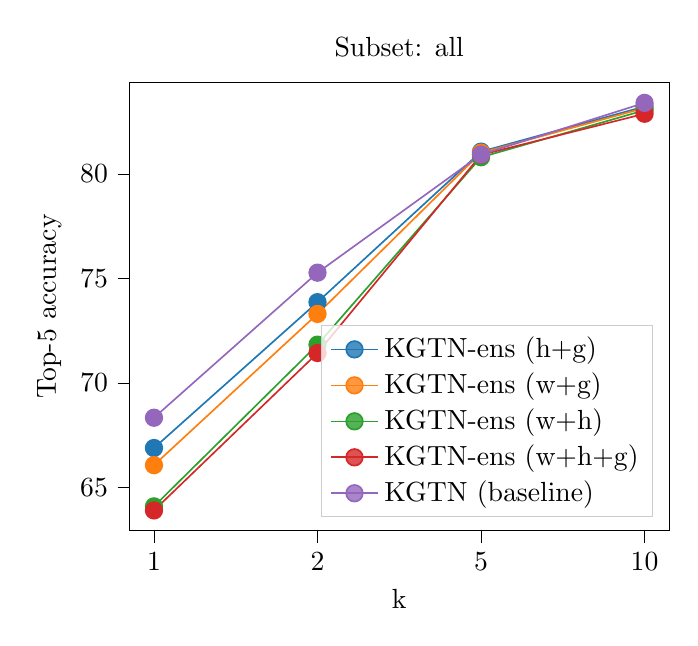
\begin{tikzpicture}

\definecolor{color0}{rgb}{0.12156862745098,0.466666666666667,0.705882352941177}
\definecolor{color1}{rgb}{1,0.498039215686275,0.0549019607843137}
\definecolor{color2}{rgb}{0.172549019607843,0.627450980392157,0.172549019607843}
\definecolor{color3}{rgb}{0.83921568627451,0.152941176470588,0.156862745098039}
\definecolor{color4}{rgb}{0.580392156862745,0.403921568627451,0.741176470588235}

\begin{axis}[
legend cell align={left},
legend style={
  fill opacity=0.8,
  draw opacity=1,
  text opacity=1,
  at={(0.97,0.03)},
  anchor=south east,
  draw=white!80!black
},
tick align=outside,
tick pos=left,
title={Subset: all},
x grid style={white!69.0196078431373!black},
xlabel={k},
xmin=-0.15, xmax=3.15,
xtick style={color=black},
xtick={0,1,2,3},
xtick={0,1,2,3},
xtick={0,1,2,3},
xtick={0,1,2,3},
xtick={0,1,2,3},
xticklabels={1,2,5,10},
xticklabels={1,2,5,10},
xticklabels={1,2,5,10},
xticklabels={1,2,5,10},
xticklabels={1,2,5,10},
y grid style={white!69.0196078431373!black},
ylabel={Top-5 accuracy},
ymin=62.9266272189349, ymax=84.3712031558185,
ytick style={color=black}
]
\addplot [semithick, color0, mark=*, mark size=3, mark options={solid}]
table {%
0 66.8867850098619
1 73.8642998027613
2 81.0642998027613
3 83.222090729783
};
\addlegendentry{KGTN-ens (h+g)}
\addplot [semithick, color1, mark=*, mark size=3, mark options={solid}]
table {%
0 66.0670611439842
1 73.301775147929
2 81.0114398422091
3 83.1502958579882
};
\addlegendentry{KGTN-ens (w+g)}
\addplot [semithick, color2, mark=*, mark size=3, mark options={solid}]
table {%
0 64.0954635108481
1 71.8303747534517
2 80.7952662721894
3 83.0429980276134
};
\addlegendentry{KGTN-ens (w+h)}
\addplot [semithick, color3, mark=*, mark size=3, mark options={solid}]
table {%
0 63.9013806706114
1 71.4319526627219
2 80.908875739645
3 82.8757396449704
};
\addlegendentry{KGTN-ens (w+h+g)}
\addplot [semithick, color4, mark=*, mark size=3, mark options={solid}]
table {%
0 68.3360946745562
1 75.2733727810651
2 80.923865877712
3 83.396449704142
};
\addlegendentry{KGTN (baseline)}
\end{axis}

\end{tikzpicture}

%         % \caption{Subset: all}
%         \label{fig:mean_all}
%     \end{subfigure}
%     \hfill
%     \begin{subfigure}[b]{.5\textwidth}
%         \centering
%         % This file was created with tikzplotlib v0.9.15.
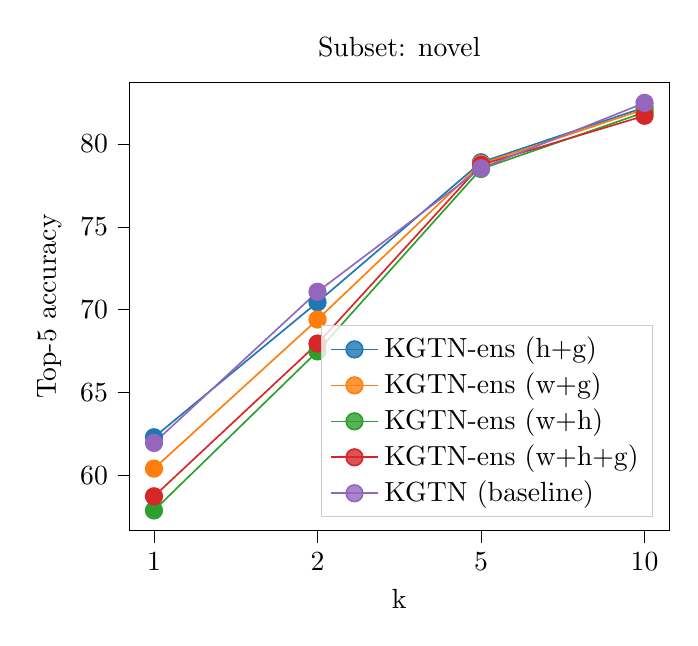
\begin{tikzpicture}

\definecolor{color0}{rgb}{0.12156862745098,0.466666666666667,0.705882352941177}
\definecolor{color1}{rgb}{1,0.498039215686275,0.0549019607843137}
\definecolor{color2}{rgb}{0.172549019607843,0.627450980392157,0.172549019607843}
\definecolor{color3}{rgb}{0.83921568627451,0.152941176470588,0.156862745098039}
\definecolor{color4}{rgb}{0.580392156862745,0.403921568627451,0.741176470588235}

\begin{axis}[
legend cell align={left},
legend style={
  fill opacity=0.8,
  draw opacity=1,
  text opacity=1,
  at={(0.97,0.03)},
  anchor=south east,
  draw=white!80!black
},
tick align=outside,
tick pos=left,
title={Subset: novel},
x grid style={white!69.0196078431373!black},
xlabel={k},
xmin=-0.15, xmax=3.15,
xtick style={color=black},
xtick={0,1,2,3},
xtick={0,1,2,3},
xtick={0,1,2,3},
xtick={0,1,2,3},
xtick={0,1,2,3},
xticklabels={1,2,5,10},
xticklabels={1,2,5,10},
xticklabels={1,2,5,10},
xticklabels={1,2,5,10},
xticklabels={1,2,5,10},
y grid style={white!69.0196078431373!black},
ylabel={Top-5 accuracy},
ymin=56.6570418006431, ymax=83.7120900321543,
ytick style={color=black}
]
\addplot [semithick, color0, mark=*, mark size=3, mark options={solid}]
table {%
0 62.3009646302251
1 70.4514469453376
2 78.8977491961415
3 82.2109324758842
};
\addlegendentry{KGTN-ens (h+g)}
\addplot [semithick, color1, mark=*, mark size=3, mark options={solid}]
table {%
0 60.4102893890675
1 69.4083601286174
2 78.8051446945338
3 82.096463022508
};
\addlegendentry{KGTN-ens (w+g)}
\addplot [semithick, color2, mark=*, mark size=3, mark options={solid}]
table {%
0 57.8868167202572
1 67.4855305466238
2 78.4926045016077
3 81.912540192926
};
\addlegendentry{KGTN-ens (w+h)}
\addplot [semithick, color3, mark=*, mark size=3, mark options={solid}]
table {%
0 58.7382636655949
1 67.9549839228296
2 78.7421221864952
3 81.7028938906752
};
\addlegendentry{KGTN-ens (w+h+g)}
\addplot [semithick, color4, mark=*, mark size=3, mark options={solid}]
table {%
0 61.9614147909968
1 71.0829581993569
2 78.5337620578778
3 82.4823151125402
};
\addlegendentry{KGTN (baseline)}
\end{axis}

\end{tikzpicture}

%         % \caption{Subset: novell}
%         \label{fig:mean_novel}
%     \end{subfigure}
%     \caption{KNGT-ens mean}
%     \label{fig:three graphs}
% \end{figure}

\begin{table*}
    \centering
    \caption{Ablation on different similarity functions used in KGTN-ens, top-5 accuracy.}
    \label{tab:results_cosine}
    \begin{tabular}{llrrrrrrrr}
    \toprule
    \multicolumn{2}{l}{} & \multicolumn{4}{c}{novel} & \multicolumn{4}{c}{all} \\ \cmidrule(lr){3-6} \cmidrule(lr){7-10}
    \multicolumn{1}{c}{type} & \multicolumn{1}{c}{knowledge graphs} & \multicolumn{1}{c}{1} & \multicolumn{1}{c}{2} & \multicolumn{1}{c}{5} & \multicolumn{1}{c}{10} & \multicolumn{1}{c}{1} & \multicolumn{1}{c}{2} & \multicolumn{1}{c}{5} & \multicolumn{1}{c}{10} \\
    
    \midrule
       KGTN &                      glove & 61.96 & 71.08 & 78.53 & 82.48 & 68.34 & 75.27 & 80.92 & 83.40 \\\cmidrule(lr){2-10}
       \multirow{4}{*}{KGTN-ens (inner prod.)} & hierarchy + glove & \textbf{62.73} & \textbf{71.48} & \textbf{78.83} & \textbf{82.56} & \textbf{68.58} & \textbf{75.45} & \textbf{81.12} & \textbf{83.46}  \\
       & wiki + glove & 61.21 & 70.66 & 78.60 & 82.34 & 67.69 & 75.04 & 80.95 & 83.33  \\
       & wiki + hierarchy + glove & 61.32 & 70.77 & 78.70 & 82.38 & 67.85 & 75.06 & 81.06 & 83.35  \\
       & wiki + hierarchy & 58.77 & 69.17 & 78.44 & 82.25 & 66.17 & 74.01 & 80.86 & 83.26  \\\cmidrule(lr){2-10}
       \multirow{4}{*}{KGTN-ens (cosine sim.)} &       hierarchy + glove & 59.57 & 69.40 & 77.29 & 81.89 & 64.86 & 73.72 & 80.05 & \textbf{83.46} \\
        &            wiki + glove & 58.34 & 68.75 & 77.24 & 81.84 & 64.43 & 73.44 & 80.01 & 83.38 \\
        &  wiki + hierarchy + glove & 57.75 & 68.44 & 77.20 & 81.90& 63.81 & 73.12 & 79.99 & 83.44 \\
        &        wiki + hierarchy & 57.35 & 68.50 & 77.27 & 81.90  & 63.87 & 73.23 & 80.00 & 83.43 \\

    \bottomrule
    \end{tabular}
    \end{table*}
    
\section{Conclusion}
\label{sec:conclusion}

In this work, we proposed KGTN-ens, which builds on KGTN and allows the incorporation of multiple knowledge sources in order to achieve better performance.
We evaluated KGTN-ens on the ImageNet-FS dataset and showed that it outperforms KGTN in most of the tested settings.
We also evaluated Wikidata embeddings in the same task and showed that they are not as effective as the other embeddings.
We believe that the proposed approach can be used in other few-shot learning tasks and we plan to test it in the future.
Although not publicly available at the time of writing this article, further work might include an evaluation of the proposed approach on ImageNet-6K dataset \cite[]{chen2020knowledge}.
A certain limitation of this study is the fact that it might not scale well for extreme classification problems, due to the calculation of pairwise distances of nodes from large knowledge graphs requiring quadratic memory complexity.
\section*{Acknowledgements}
This research was co-funded by Interreg \"Osterreich-Bayern 2014-2020 programme project KI-Net: Bausteine f\"ur KI-basierte Optimierungen in der industriellen Fertigung (grant agreement: AB 292).


% To print the credit authorship contribution details
\printcredits

%% Loading bibliography style file
%\bibliographystyle{model1-num-names}
\bibliographystyle{cas-model2-names}

% Loading bibliography database
\bibliography{bibliography}

% Biography
\bio{}
% Here goes the biography details.
\endbio

% \bio{pic1}
% % Here goes the biography details.
% \endbio

\end{document}
